\documentclass[a4paper]{article}

% CJK support: prefer ctex, fallback to XeTeX native line breaking
\IfFileExists{ctex.sty}{
  \usepackage[fontset=fandol]{ctex}
}{
  \usepackage{fontspec}
  \XeTeXlinebreaklocale "zh"
  \XeTeXlinebreakskip = 0pt plus 1pt
  \IfFontExistsTF{Songti SC}{\setmainfont{Songti SC}}{%
    \IfFontExistsTF{Noto Serif CJK SC}{\setmainfont{Noto Serif CJK SC}}{}%
  }
  \IfFontExistsTF{Heiti SC}{\setsansfont{Heiti SC}}{%
    \IfFontExistsTF{Noto Sans CJK SC}{\setsansfont{Noto Sans CJK SC}}{}%
  }
}

\usepackage{amsmath, amssymb}
\usepackage{graphicx}
\usepackage[margin=2.5cm]{geometry}
\usepackage[most]{tcolorbox}
\usepackage{etoolbox}
\usepackage{listings}
\usepackage{hyperref}
\usepackage{booktabs}
\usepackage{subcaption}
\usepackage{float}
\usepackage{tikz}
\IfFileExists{pgfplots.sty}{
    \usepackage{pgfplots}
    \pgfplotsset{compat=1.18}
}{}

\newtcolorbox{knowledgebox}[1]{
    enhanced, colback=blue!5!white, colframe=blue!75!black, colbacktitle=blue!75!black,
    coltitle=white, fonttitle=\bfseries, title=#1, attach boxed title to top left={yshift=-2mm, xshift=2mm},
    boxrule=1pt, sharp corners
}

\newtcolorbox{importantbox}[1]{
    enhanced, colback=yellow!10!white, colframe=yellow!80!black, colbacktitle=yellow!80!black,
    coltitle=black, fonttitle=\bfseries, title=#1, sharp corners
}

\newtcolorbox{warningbox}[1]{
    enhanced, colback=red!5!white, colframe=red!75!black, colbacktitle=red!75!black,
    coltitle=white, fonttitle=\bfseries, title=#1, sharp corners
}

\lstset{
    basicstyle=\ttfamily\small,
    keywordstyle=\color{blue},
    stringstyle=\color{red!60!black},
    commentstyle=\color{green!60!black},
    breaklines=true,
    frame=single,
    numbers=left,
    numberstyle=\tiny\color{gray},
    captionpos=b,
    extendedchars=false
}

\newcommand{\vtag}{\protect\footnotemark}
\newcommand{\srcnote}[1]{\footnotetext{视频画面时间区间：#1。若为裁剪图，时间区间仍对应原视频画面。}}
\newcommand{\degC}{\ensuremath{^{\circ}\mathrm{C}}}
\newcommand{\um}{\ensuremath{\mu\mathrm{m}}}
\newcommand{\nm}{\ensuremath{\mathrm{nm}}}
\newcommand{\angstrom}{\ensuremath{\text{\AA}}}

\newcommand{\notetitle}{智能体的记忆与技能}
\newcommand{\notesubtitle}{CMU 11-768 AI Agents 第 4 讲：智能体如何在不重训模型的前提下越做越好}
\newcommand{\noteauthors}{讲者：Daniel Fried（片头标题页署名）\quad 笔记整理：lecture-to-notes}
\newcommand{\notedate}{2026}
\newcommand{\videochannel}{CMU 11-768 AI Agents（视频上传者 Graham Neubig）}
\newcommand{\videopublishdate}{2026 年课程录像}
\newcommand{\videoduration}{75 分 22 秒}
\newcommand{\videourl}{https://www.youtube.com/watch?v=6zigF2a-2Pw}
\newcommand{\videocoverpath}{cover.jpg}

\begin{document}

\begin{titlepage}
\centering
{\Large 课程笔记\par}
\vspace{1.2cm}
{\huge\bfseries \notetitle\par}
\ifdefempty{\notesubtitle}{}{
\vspace{0.3cm}
{\large \notesubtitle\par}
}
\vspace{0.5cm}
{\large \noteauthors\par}
\vspace{0.3cm}
{\large \notedate\par}
\vspace{1.0cm}

\ifdefempty{\videocoverpath}{
{\small 请在生成笔记时填入视频封面图的本地路径。\par}
}{
\includegraphics[width=0.82\textwidth,height=0.40\textheight,keepaspectratio]{\videocoverpath}\par
}

\vfill
\begin{tcolorbox}[width=0.9\textwidth, colback=black!2!white, colframe=black!60, sharp corners]
\textbf{视频作者/频道}：\videochannel\par
\textbf{发布日期}：\videopublishdate\par
\textbf{视频时长}：\videoduration\par
\textbf{视频链接}：
\ifdefempty{\videourl}{
未填写
}{
\href{\videourl}{\nolinkurl{\videourl}}
}
\end{tcolorbox}
\end{titlepage}

\tableofcontents
\newpage

\section{为什么要让智能体记住跨任务的经验}

上一讲处理的是任务内部的上下文管理：在有限的窗口里决定保留哪些观察、动作与反馈。本讲把问题向前推一步。一个任务结束、窗口被清空之后，智能体能不能把这次学到的东西留下来，让未来的任务受益？如果只能靠窗口，那么每开一个新任务，之前摸索出来的做法就会一起归零。

视频用一个购物网站的例子开场。用户先要求把 Sony 耳机加入愿望清单，之后又要求查询无线键盘的价格区间。两个目标不同，但都要打开同一家商店、找到搜索框、输入关键词并点击搜索。真正被复用的就是这一段搜索子过程，而任务专属的部分只在结尾：一个把结果加入愿望清单，另一个读取价格并汇报。图~图 1 画出了这条共享结构。

\begin{figure}[H]
\centering
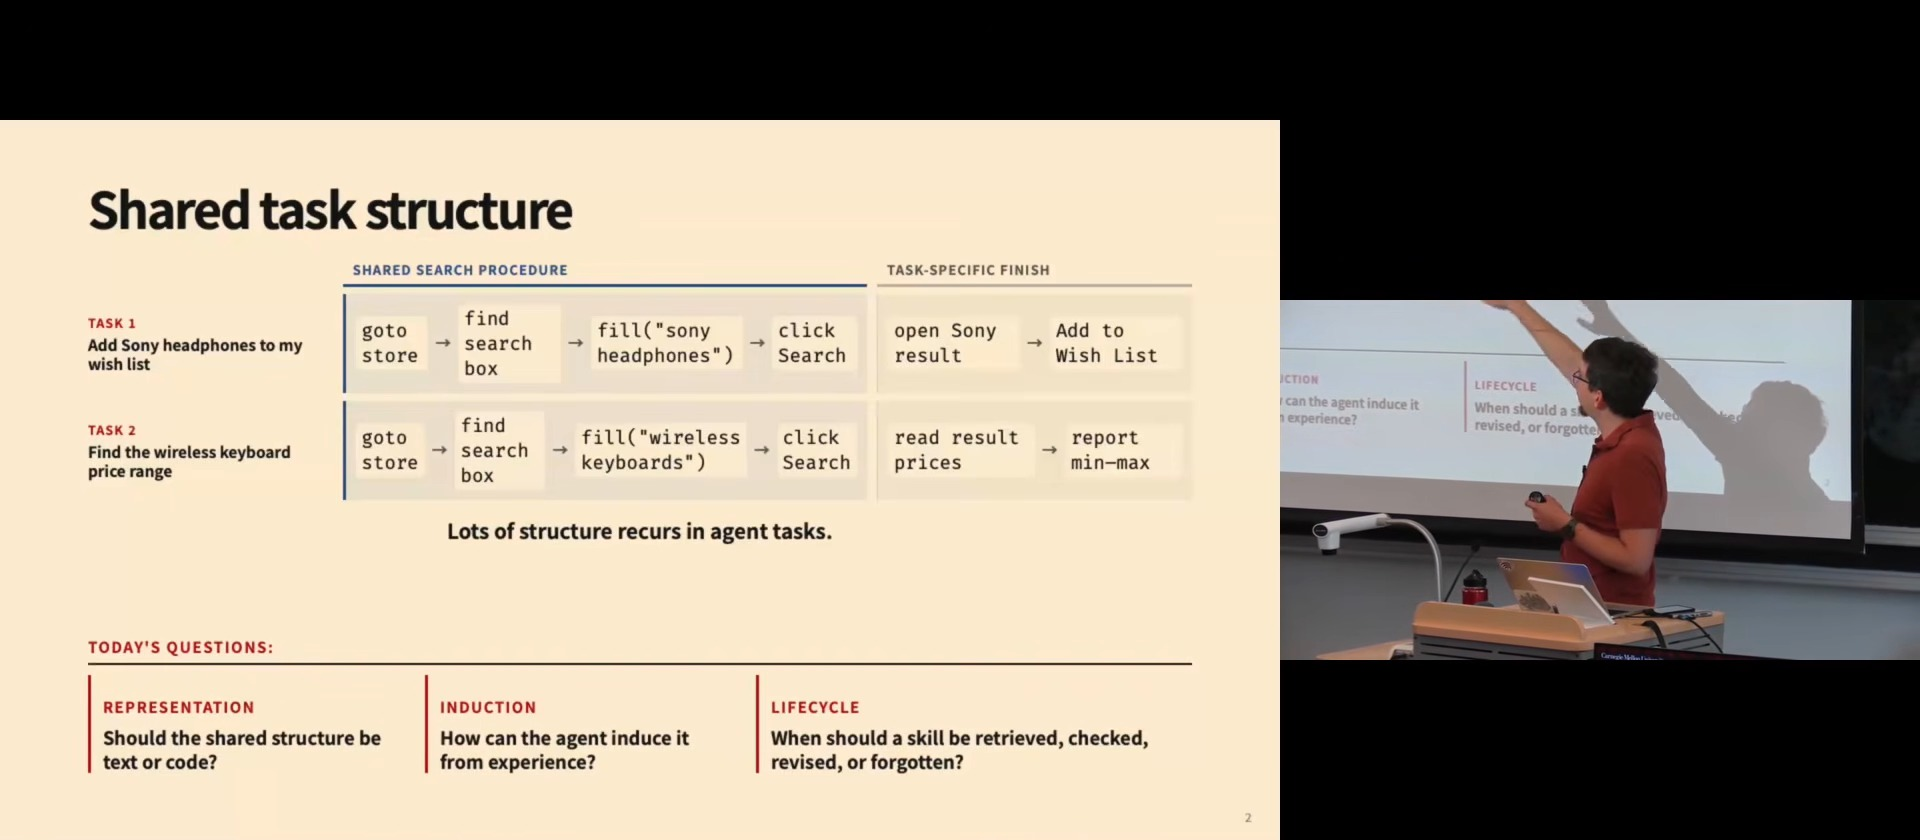
\includegraphics[width=\textwidth]{figures/fig_01_shared_task_structure.jpg}
\caption{购物网站两个任务共享的搜索子过程与任务专属收尾：定位搜索框、填入查询、点击搜索按钮这一段可以复用\vtag}

\end{figure}
\srcnote{00:03:30--00:03:45}

一旦承认“共享结构会反复出现”，设计问题就变成：经验应该改在系统的哪个位置？视频列出三种位置，并逐项比较利弊，如图~图 2 所示。第一种是上下文窗口，也就是上一讲反复讨论的地方；它最贴近真实发生的步骤，但代价是昂贵、含噪，而且模型还得自己判断哪些内容重要。第二种是外部工件，例如数据库记录或文件系统里的文本与代码；它可检查、可编辑、可检索，也能跨模型移植，但必须有人或智能体去归纳、筛选和维护。第三种是模型权重，也就是监督微调或强化学习；它让推理更快、行为改变更广，但更新更慢、过程不透明，而且只对特定模型生效。

\begin{figure}[H]
\centering
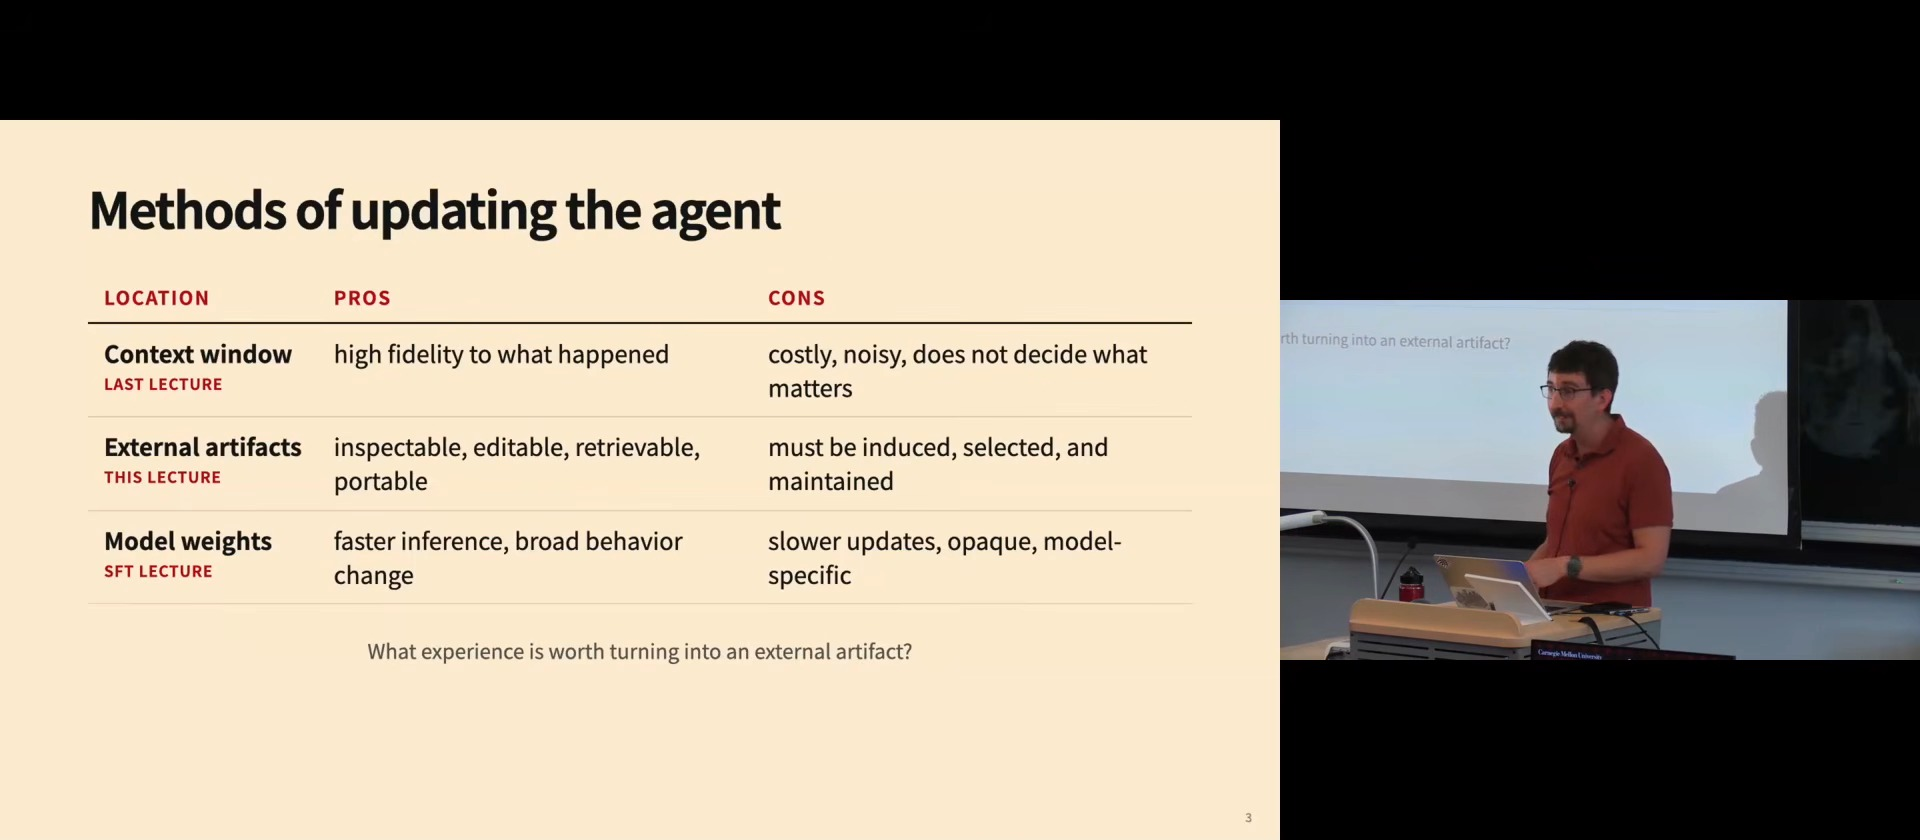
\includegraphics[width=\textwidth]{figures/fig_02_update_locations.jpg}
\caption{上下文窗口、外部工件与模型权重三种更新位置的优缺点对照，三列分别标注为上一讲、本讲与后续微调讲\vtag}

\end{figure}
\srcnote{00:08:15--00:08:30}

\begin{importantbox}{为什么讲者更偏向外部工件}
外部工件有两个窗口和权重都给不了的性质。第一是\textbf{可移植}：一段“如何在这家网站搜索”的说明，可以被同一个智能体框架下的多个模型使用；权重更新只属于被更新的那个模型。第二是\textbf{可检查}：人可以直接阅读、修改智能体写下的说明，也可以把自己的最佳实践写成文本交给智能体，人和系统之间因此有了一个可协商的接口。
\end{importantbox}

不过，可检查与可移植并不等于免费。外部工件需要被归纳、筛选和维护，而这正是本讲后半程的主要内容。

\begin{warningbox}{不要把外部存储想成自动获益}
把经验写进文件并不自动提升表现。写什么、什么时候写、写进去以后怎么用，每一步都可能出错。本讲后面会看到：技能加得太多会分散模型注意力；记忆里存了错误的轨迹会把模型带偏；裁判判错会把坏经验写进记忆；检索到不相关的经验甚至会让成功率下降。
\end{warningbox}

外部记忆解决的是容量问题，但要让它真的被用上，工作上下文必须先被填充。本讲义把这一机制压缩成一个记号：

\[
C_t = S \;\Vert\; R(M_{\text{ext}}, q_t) \;\Vert\; O_t
\]

\begin{itemize}
\item $C_t$：第 $t$ 步送进语言模型的上下文；
\item $S$：系统指令，通常是只读的固定前缀；
\item $M_{\text{ext}}$：上下文窗口之外的外部记忆；
\item $q_t$：当前任务的描述或查询；
\item $R$：检索算子，把外部记忆中与 $q_t$ 相关的内容取回；
\item $O_t$：本轮工具调用返回的观察；
\item $\Vert$：按顺序拼接。
\end{itemize}

这个记号来自讲者对 MemGPT 一类系统的口述说明，本讲义把它显式写出，用来提醒一件事：外部记忆本身不参与推理，只有被检索进 $C_t$ 的部分才会影响模型。

\subsection{本章小结}

外部工件把经验从一次任务的窗口里解放出来，代价是必须被主动管理和维护。接下来的问题是：外部存储里到底该放哪几类东西。这是下一节的分类问题。

\section{值得保留的三种经验}

外部存储不是无差别的仓库。视频把可保留的经验分成三类，并为每一类给出判据，如图~图 3 所示。

\begin{figure}[H]
\centering
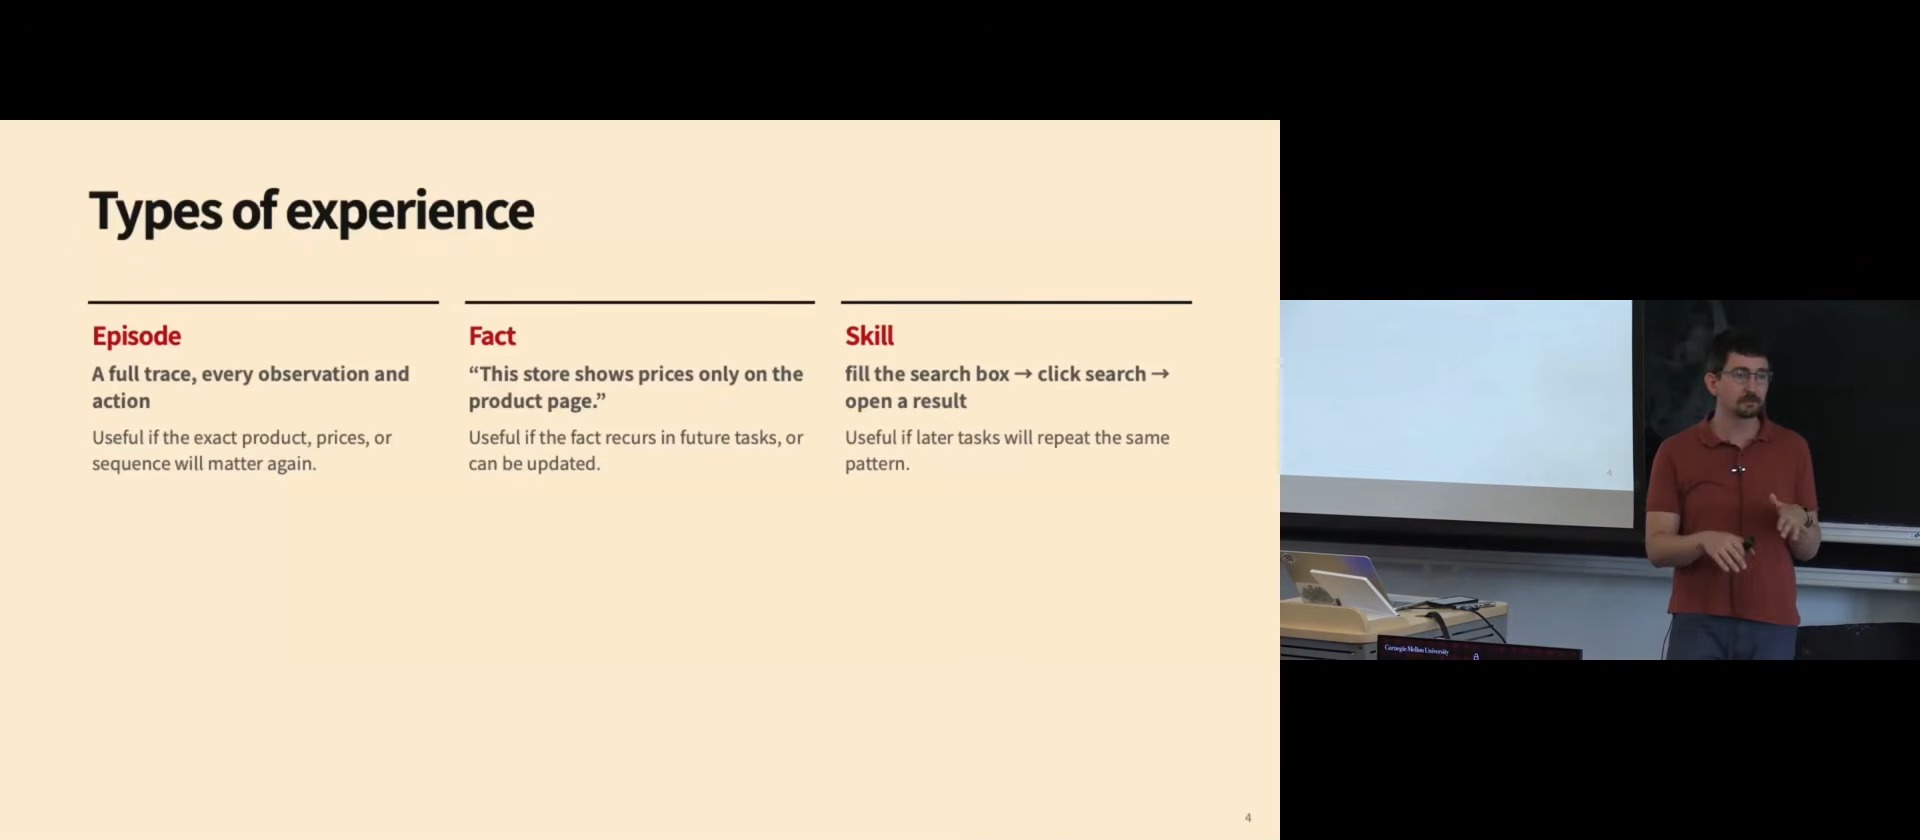
\includegraphics[width=\textwidth]{figures/fig_03_experience_types.jpg}
\caption{Episode、Fact、Skill 三类可保留经验的定义与适用判据\vtag}

\end{figure}
\srcnote{00:11:15--00:11:30}

\begin{table}[H]
\centering
\caption{三类经验的判据与例子（据视频第 7 页整理）}
\begin{tabular}{p{2.6cm}p{5.3cm}p{5.3cm}}
\toprule
类型 & 是什么 & 什么时候值得留 \\
\midrule
Episode & 一次完整的观察与动作轨迹 & 当具体商品、价格或步骤序列还会再次出现时 \\
Fact & 关于环境或用户的事实 & 当事实会反复用到，或者需要被更新时 \\
Skill & 如何完成某个子过程 & 当后续任务会重复同一模式时 \\
\bottomrule
\end{tabular}
\end{table}三个判据其实在回答同一件事：未来任务与这段经验的\textbf{重叠程度}。整条轨迹保真度最高，也最贵，而且绝大多数细节不会被再次用到，因此视频明确说“不需要全部保留”。事实是最早被研究的形态，聊天助手的记忆设置就属于这一类：用户说过自己住在哪里、从事什么工作，系统把这类事实抽成文本存下来，日后重新取用。技能是最后一类，也是与智能体最相关的一类：它把“如何做”从“这次做的具体内容”里剥出来。

\begin{knowledgebox}{记忆与技能的边界}
视频用一页对照把两者分开，如图~图 4 所示。记忆是从智能体自身交互中保存下来的内容，例如“上次买过某个商品”；技能是关于“该如何行动”的可复用知识，可以用文本、代码或两者混合表示，例如人写下的一份发布前检查清单，或智能体从自己成功搜索中归纳出的做法。
\end{knowledgebox}

\begin{figure}[H]
\centering
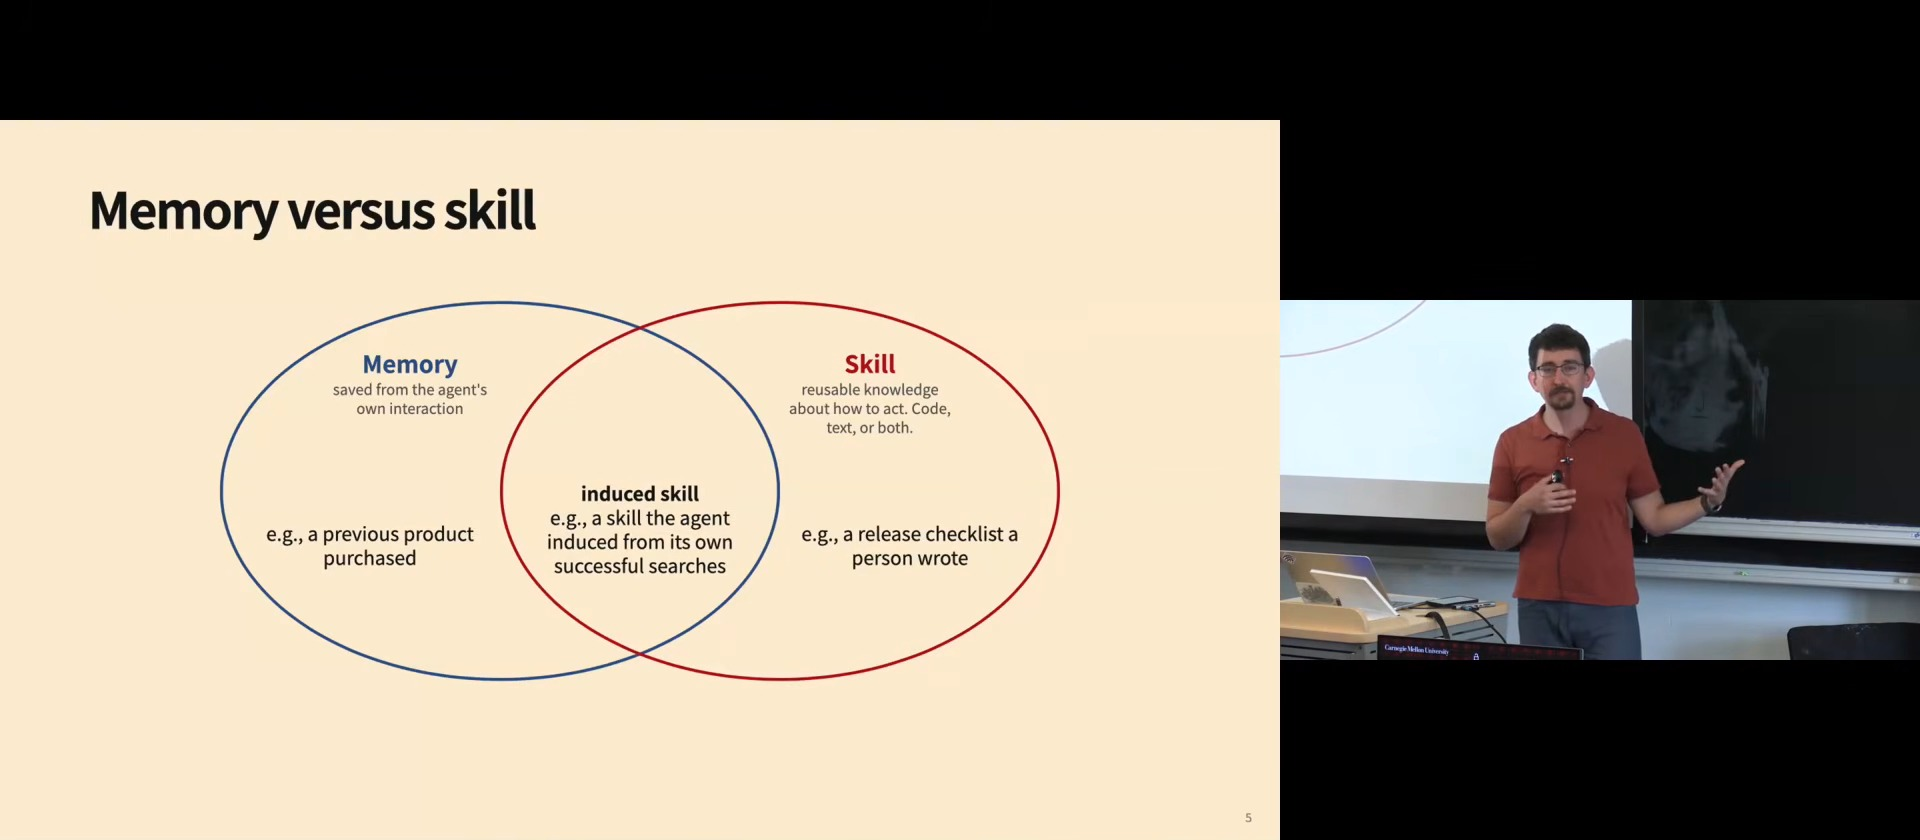
\includegraphics[width=\textwidth]{figures/fig_04_memory_vs_skill.jpg}
\caption{记忆与技能的区别：记忆保存交互所得，技能是可复用的行动知识，载体可以是代码、文本或两者\vtag}

\end{figure}
\srcnote{00:12:30--00:12:45}

技能是否值得存在，取决于同一个子任务是否会被反复执行。视频把这一点说得很直接：如果一段子过程只做一次，把它固化成技能只是增加负担；只有重复出现时，技能才可能摊薄它的编写与维护成本。这也解释了为什么代码审查、升级依赖、发布上线这类流程特别适合做成技能：它们的规格相对固定，而且会一再发生。

人工技能与学习技能是两条互补的路线。人工技能的来源清楚、质量可控，适合承载组织政策和个人偏好，代价是编写与维护都要花人力。学习技能由智能体从自己的经历中归纳，可以自动化地形成闭环，代价是可能含噪，尤其在把技能交给另一个智能体使用时，可能出现意料之外的后果。

\begin{importantbox}{技能是“固定规格”的容器}
视频的判据是：当你要反复做一件事，并且它遵循一套固定的规格时，就应该考虑技能。技能把这份规格从一次次的对话里拿出来，变成一份可复用的文本。至于规格在具体情境中怎么落实，仍然交给模型判断。
\end{importantbox}

\begin{warningbox}{Episode 的隐藏成本}
完整轨迹保真度最高，但它同时占用最多上下文，也最可能把与当前任务无关的细节带进来。判据是未来任务与这段经验的重叠程度，而不是这段经验本身有多完整。把整条轨迹当作默认选择，通常会让记忆迅速变得又长又吵。
\end{warningbox}

\subsection{本章小结}

Episode、Fact、Skill 覆盖了从“这次发生了什么”到“以后该怎么做”的连续谱。其中技能最需要设计决策，因为它既要表达做法，又要在新环境里保持可用。下一节先看已经被广泛采用的人工技能格式，以及它如何用渐进披露控制上下文开销。

\section{人工编写的技能：格式与渐进披露}

\subsection{什么样的请求应该固化成技能}

视频用代码审查举例：一个人如果每次都在对话里粘贴同一段要求，就说明这段要求适合写成技能。图~图 5 展示了这段被反复输入的请求，包括用 Black 格式化并限制 88 列、用自定义规则跑 Ruff、为所有公开 API 加类型标注、使用 Google 风格文档字符串、以及为新函数补 Pytest。

\begin{figure}[H]
\centering
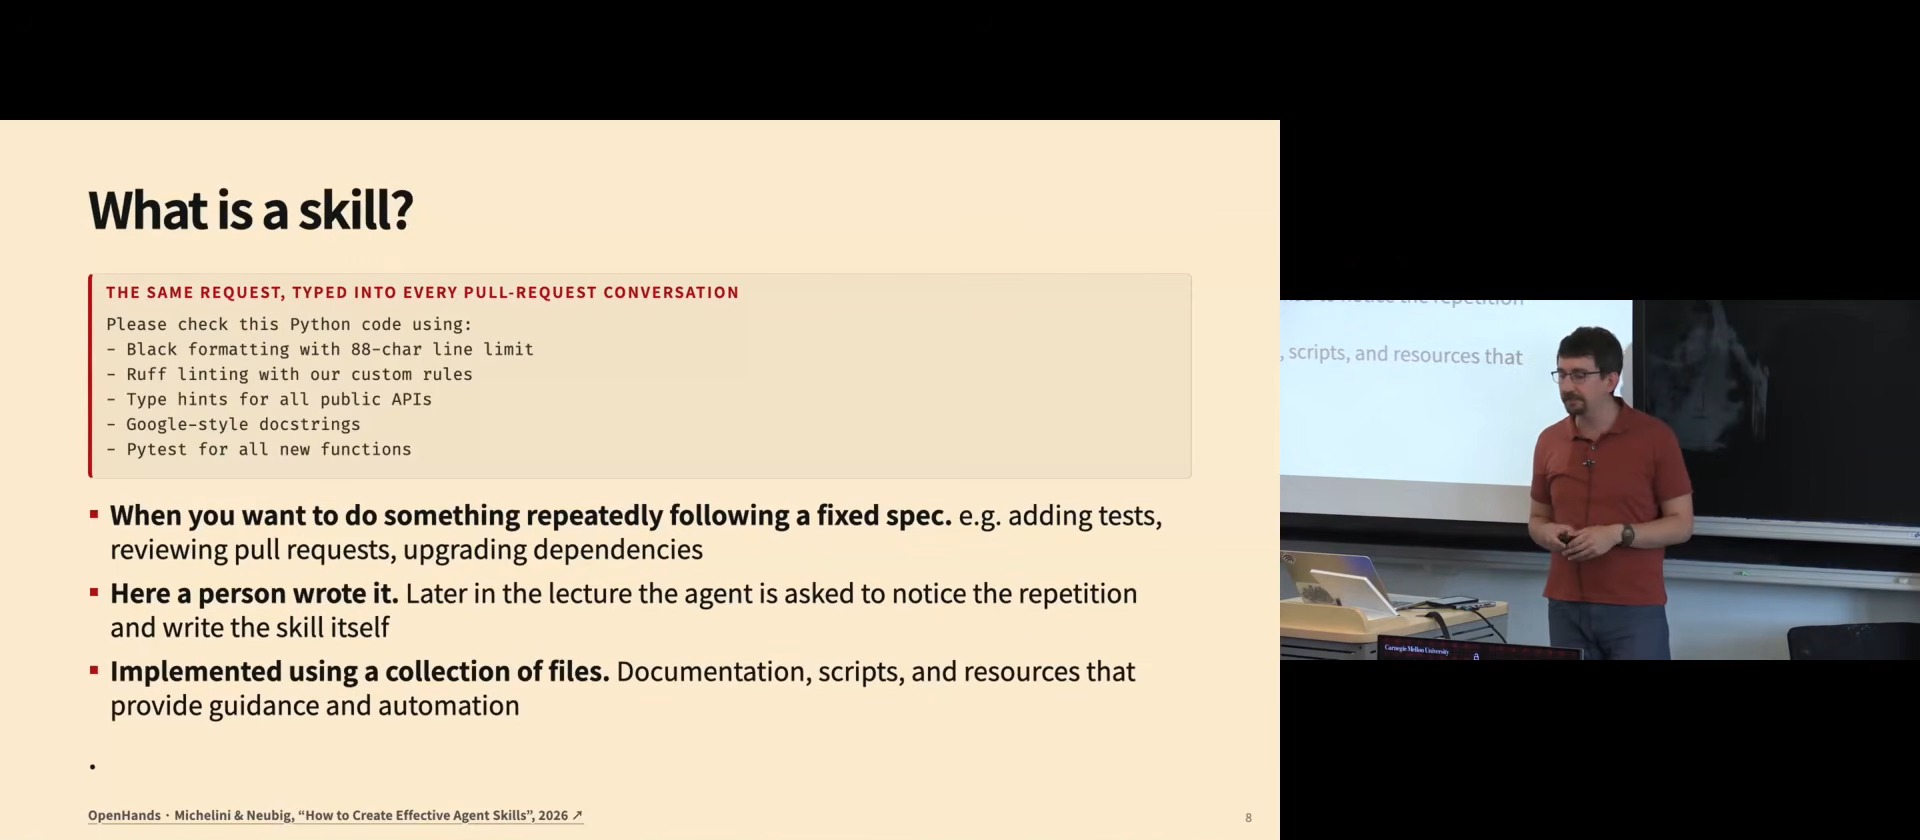
\includegraphics[width=\textwidth]{figures/fig_05_what_is_a_skill.jpg}
\caption{把反复输入的代码审查要求写成一个技能：固定规格、重复执行，例如加测试、审查拉取请求、升级依赖\vtag}

\end{figure}
\srcnote{00:15:30--00:15:45}

这些要求有一个共同点：它们描述的是流程，而不是某一次代码的具体问题。人写技能时知道自己的意图和出处，质量更容易控制；但写和维护都要花时间。当技能由智能体生成时，从任务描述凭空造技能的效果很差，视频引用的评测甚至显示这样做会让表现变差。可行的做法是让技能紧跟在一次真实工作流之后产生，因为任务过程会暴露出事先想不到的约束。

\subsection{技能包的目录结构}

当前的事实标准叫 Agent Skills。一个技能就是一个包含若干文件的目录，其中 SKILL.md 是必需的。图~图 6 展示了 python-review 技能包的布局：目录里除了 SKILL.md，还可以有 scripts（可执行代码）、references（补充文档）和 assets（模板与资源）。

\begin{figure}[H]
\centering
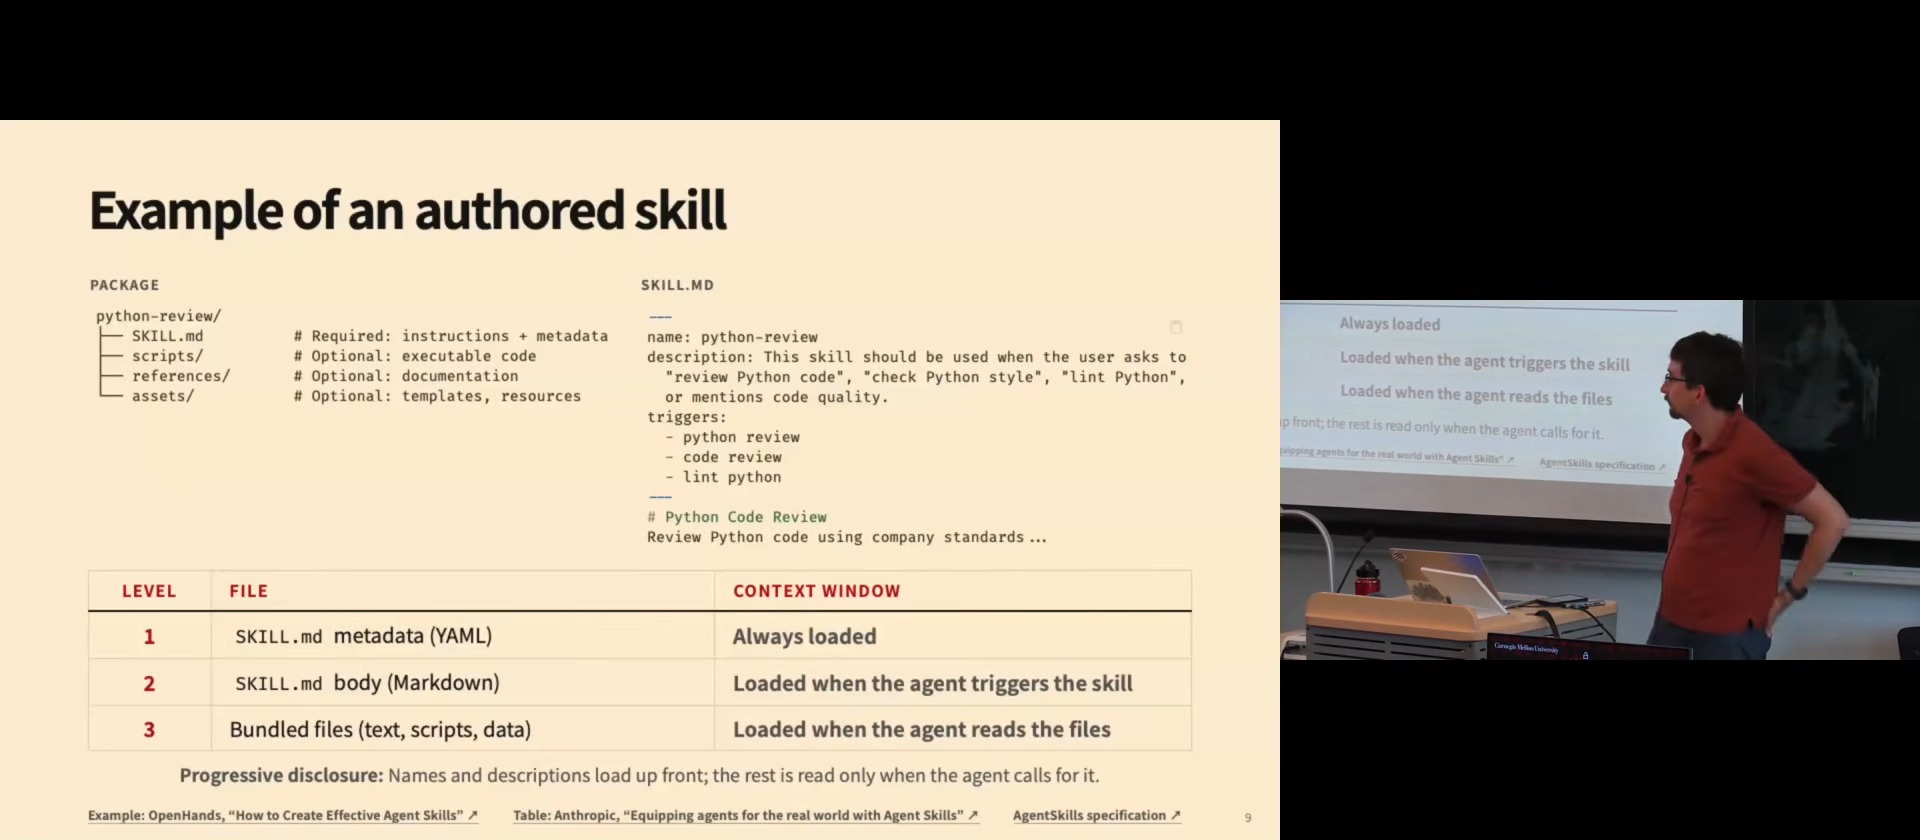
\includegraphics[width=\textwidth]{figures/fig_06_skill_package.jpg}
\caption{技能包目录结构与 SKILL.md 的必填元数据：name、description、triggers，以及 scripts、references、assets 三个可选子目录\vtag}

\end{figure}
\srcnote{00:23:15--00:23:30}

SKILL.md 的前半部分是 YAML 元数据。视频强调其中两个字段：name 是技能的稳定名称，description 用一两句话告诉模型这个技能在什么情况下适用。元数据之后是正文，写明技能被触发后应当执行哪些步骤。scripts、references、assets 都是可选的，它们存在的意义不是被一次性读完，而是当模型判断需要时再去读取。

\subsection{渐进披露：让上下文只承担当下需要的信息}

技能包可能很大，而系统不希望把成千上万个技能的全部正文都塞进上下文。视频给出的机制叫渐进披露，分三层。第一层是元数据，也就是每个技能的名称和描述；只要技能对模型可用，这一层就会出现在系统提示里。图~图 7 展示了这一层在系统提示中的样子：先说明技能是什么、如何用 skill\_view 读取正文，然后列出可用技能的索引。

\begin{figure}[H]
\centering
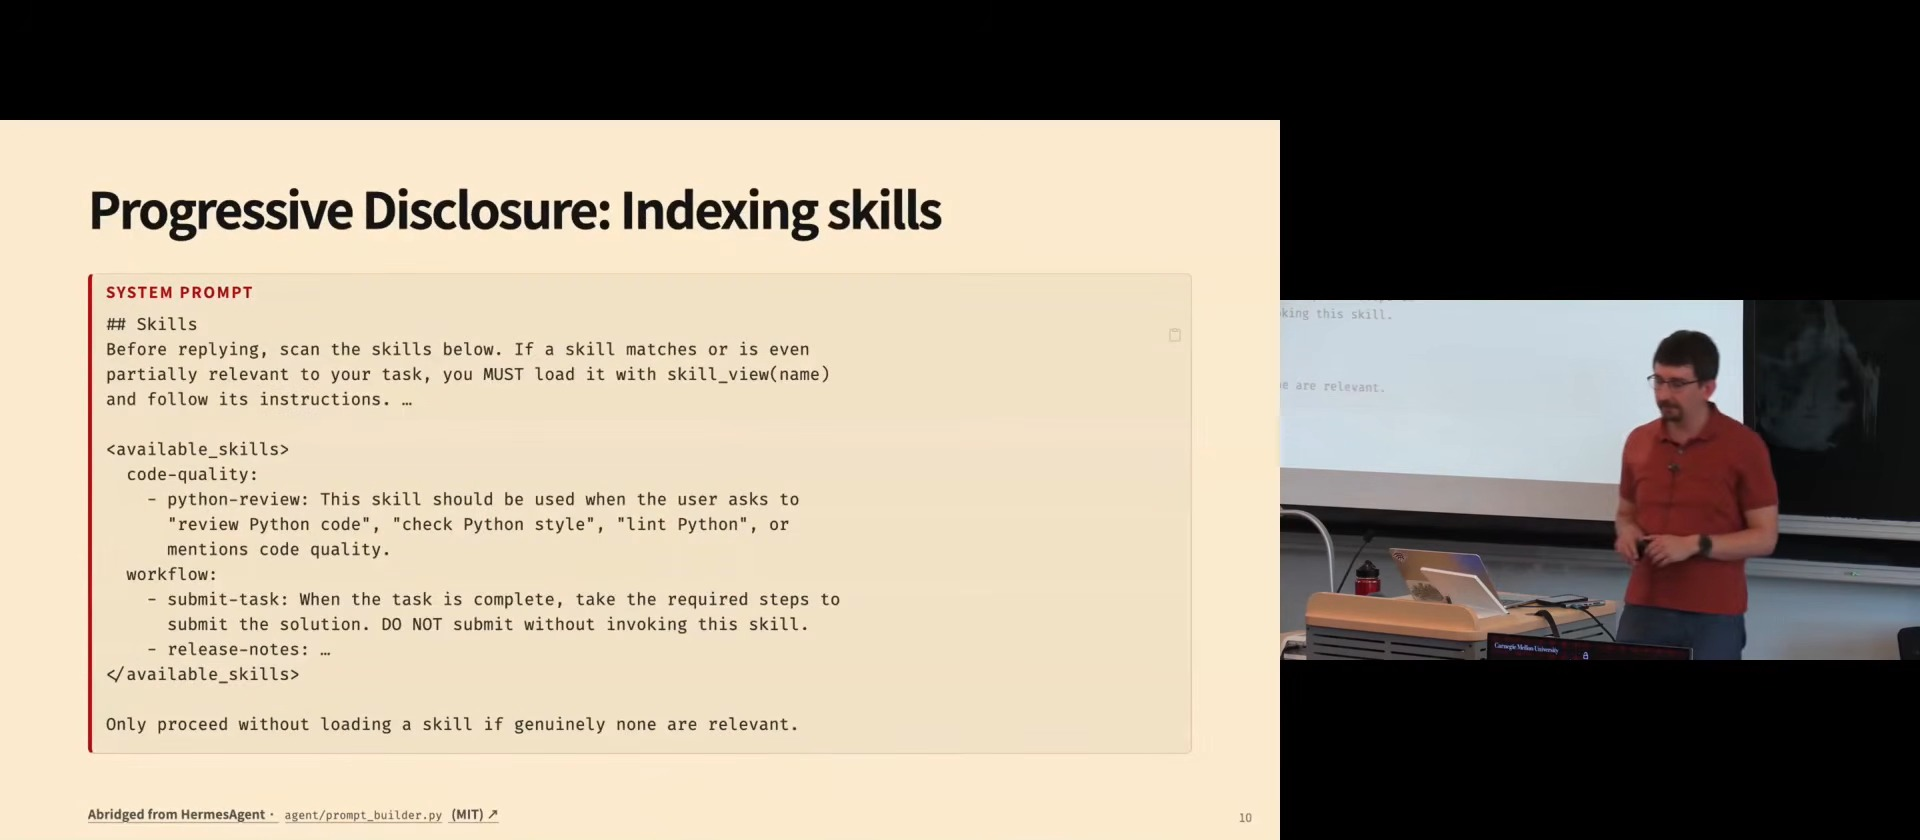
\includegraphics[width=\textwidth]{figures/fig_07_progressive_index.jpg}
\caption{渐进披露第一层：系统提示里只放技能名与描述，模型在判断相关后用 skill\_view 载入正文\vtag}

\end{figure}
\srcnote{00:24:30--00:24:45}

第二层是正文。模型判断某个技能与当前任务相关时，通过一次工具调用把 SKILL.md 的正文取回，作为工具结果进入上下文。第三层是资源，例如 scripts 里的检查脚本；模型在终端运行脚本，看到的只是脚本输出，而脚本源码本身不会进入上下文。图~图 8 把这三层按轮次列了出来：第一轮只有索引，第二轮载入正文，第三轮执行脚本并读取输出。

\begin{figure}[H]
\centering
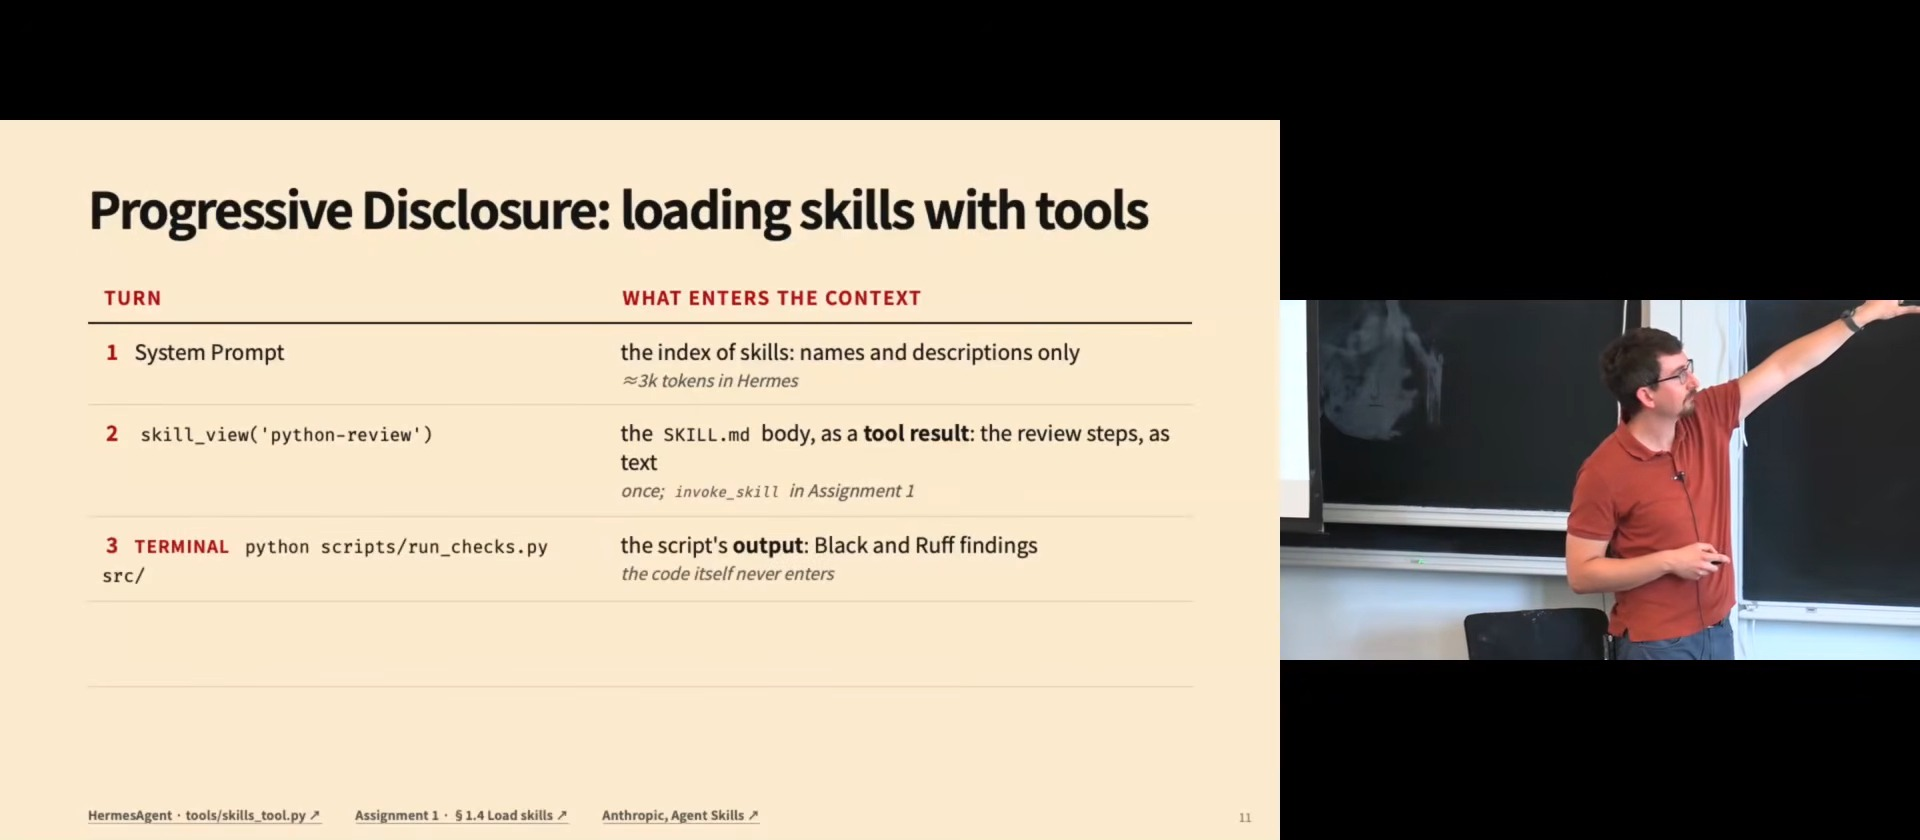
\includegraphics[width=\textwidth]{figures/fig_08_progressive_loading.jpg}
\caption{渐进披露三层：系统提示中的技能索引、用 skill\_view 载入的 SKILL.md 正文、以及终端脚本的输出；脚本源码本身不进入上下文\vtag}

\end{figure}
\srcnote{00:25:45--00:26:00}

这套分层可以用一个代价式概括。设共有 $N$ 个可用技能，第 $i$ 个技能的元数据长度为 $d_i$，被载入正文的技能集合为 $\mathcal{L}$，正文长度为 $b_j$，则常驻开销与按需开销分别是

\[
D_{\text{index}} = \sum_{i=1}^{N} d_i ,
\qquad
D_{\text{on-demand}} = \sum_{j \in \mathcal{L}} b_j .
\]

\begin{itemize}
\item $N$：可用技能的总数；
\item $d_i$：第 $i$ 个技能的元数据长度（名称与描述）；
\item $\mathcal{L}$：本轮被判定为相关、因而载入正文的技能集合；
\item $b_j$：第 $j$ 个技能的正文长度。
\end{itemize}

渐进披露的设计意图，是让 $D_{\text{index}}$ 尽量小、让 $D_{\text{on-demand}}$ 只在需要时发生。但 $D_{\text{index}}$ 仍然随 $N$ 线性增长，这正是下一段的问题。

\subsection{技能越多越好吗}

答案是否定的。视频提到，在一个先进的智能体里，系统提示中所有技能描述的总长度大约是 3,000 token；如果技能数量继续膨胀，模型会被不相关的内容干扰，表现反而下降。触发本身也不可控：是否调用 skill\_view 完全取决于模型根据上下文作出的判断，因此 description 的写法会直接影响技能能不能在正确的时机被触发。视频由此得出一个方法论上的结论：技能需要评测，不能凭感觉认为它有理。

\begin{warningbox}{两个常见误解}
第一，技能不是越多越好。即使元数据很短，数量足够多也会让上下文变长、注意力分散。第二，技能不会自动触发。触发是模型生成的工具调用，写得不清楚就可能该用的时候不用，或者在不该用的时候乱用。这两点都必须用评测来回答。
\end{warningbox}

\subsection{本章小结}

人工技能把固定规格从对话搬进文件，渐进披露则让这些文件不必一次性占用上下文。但格式正确不代表有效。下一节看不依赖于个例的评测怎么做，以及技能在什么条件下真的带来增益。

\section{技能真的有用吗：评测与维护闭环}

\subsection{SkillsBench 的评测设计}

视频介绍了一个早期的系统化评测，叫 SkillsBench。它分三个阶段：先构建基准，再对技能做质量过滤，最后跑评测，如图~图 9 所示。技能生态一侧从网络上收集了 234,896 条候选，经过过滤后保留 2,014,000 这个规模的唯一技能集合（视频中同时给出 1,773,213 与 5,891 等中间统计）；任务一侧由人工编写了 400 个看起来可能受益于技能的任务，最终在 87 个任务、8 个领域上评测。评测覆盖 18 套模型配置、142 位贡献者与 9,396 条轨迹。

\begin{figure}[H]
\centering
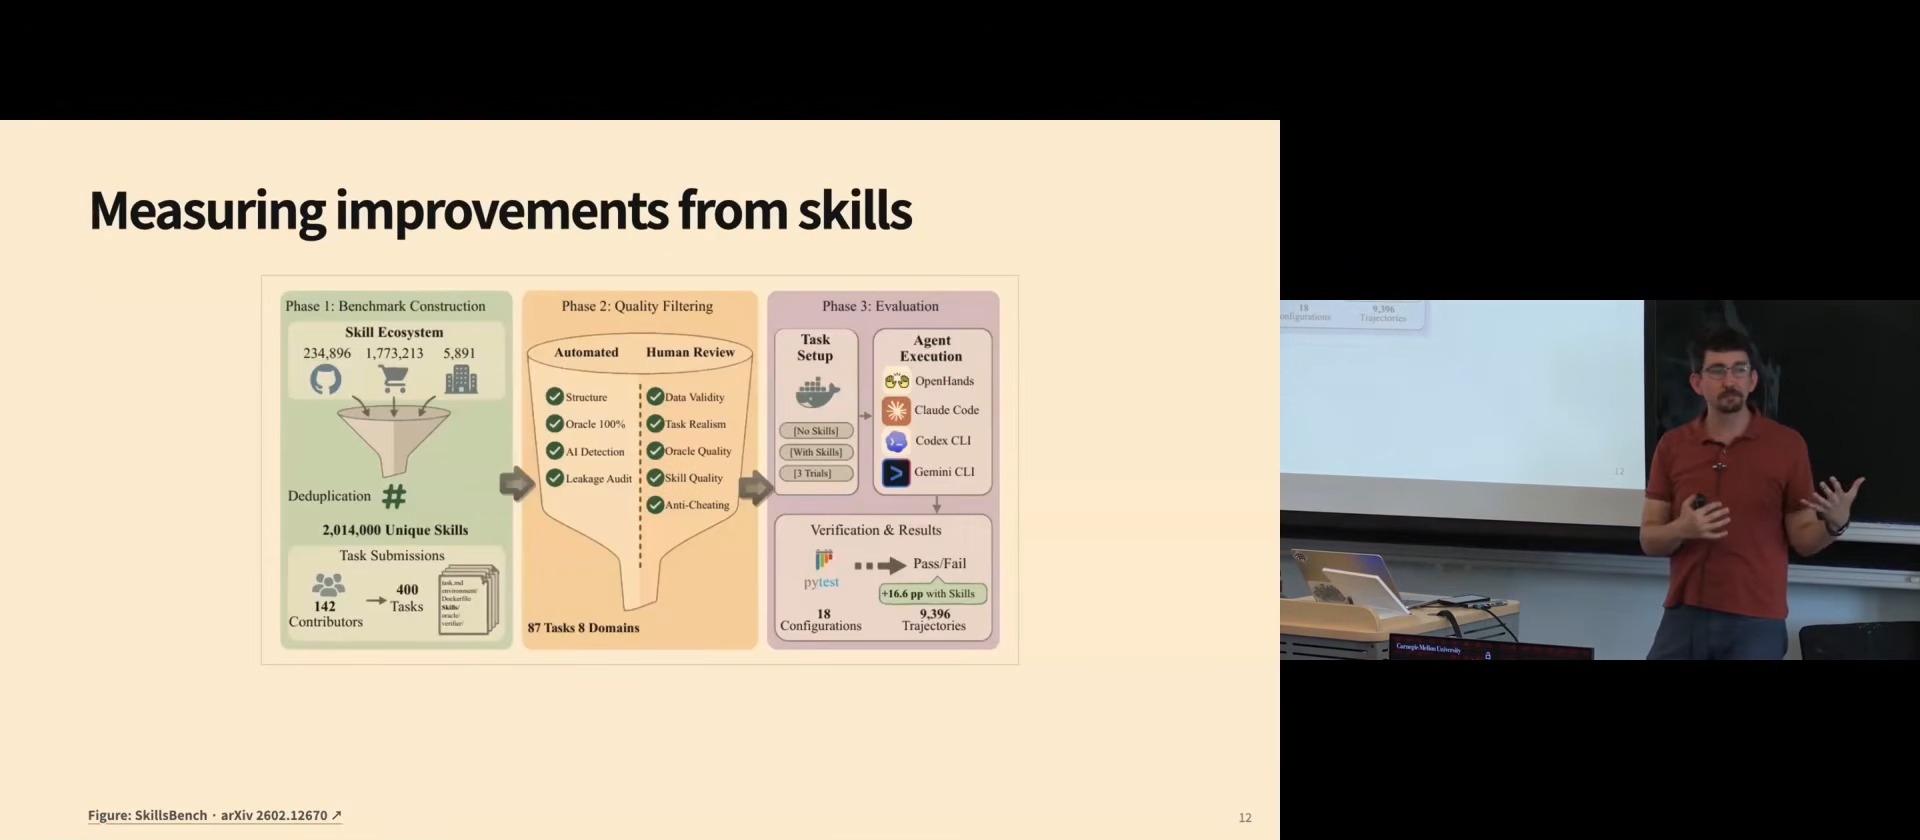
\includegraphics[width=\textwidth]{figures/fig_09_skillsbench_pipeline.jpg}
\caption{SkillsBench 的三阶段流水线：基准构建、技能质量过滤与评测；图中给出 2,014,000 个唯一技能、400 个任务与 9,396 条轨迹等规模数字\vtag}

\end{figure}
\srcnote{00:27:00--00:27:15}

任务与技能是分开编写的，再由任务标注者从技能池中挑出看起来适用的技能交给智能体。评测在四个智能体框架与十多个模型上进行，用人类编写的验证标准判断通过与否。之所以要在多个框架和模型上重复，是为了区分“技能质量好”与“这套模型和框架恰好会用技能”这两件事。

\subsection{平均增益与适用边界}

在这套受控设定下，人工技能把平均通过率从 33.9 提升到 50.5，整体上约等于 16.6 个百分点的提升。但增益并不是均匀的。图~图 10 的柱状图显示，只涉及一至三个技能的任务，收益明显大于需要四个以上技能的任务；SKILL.md 更短的技能组也表现出更大的增益。

\begin{figure}[H]
\centering
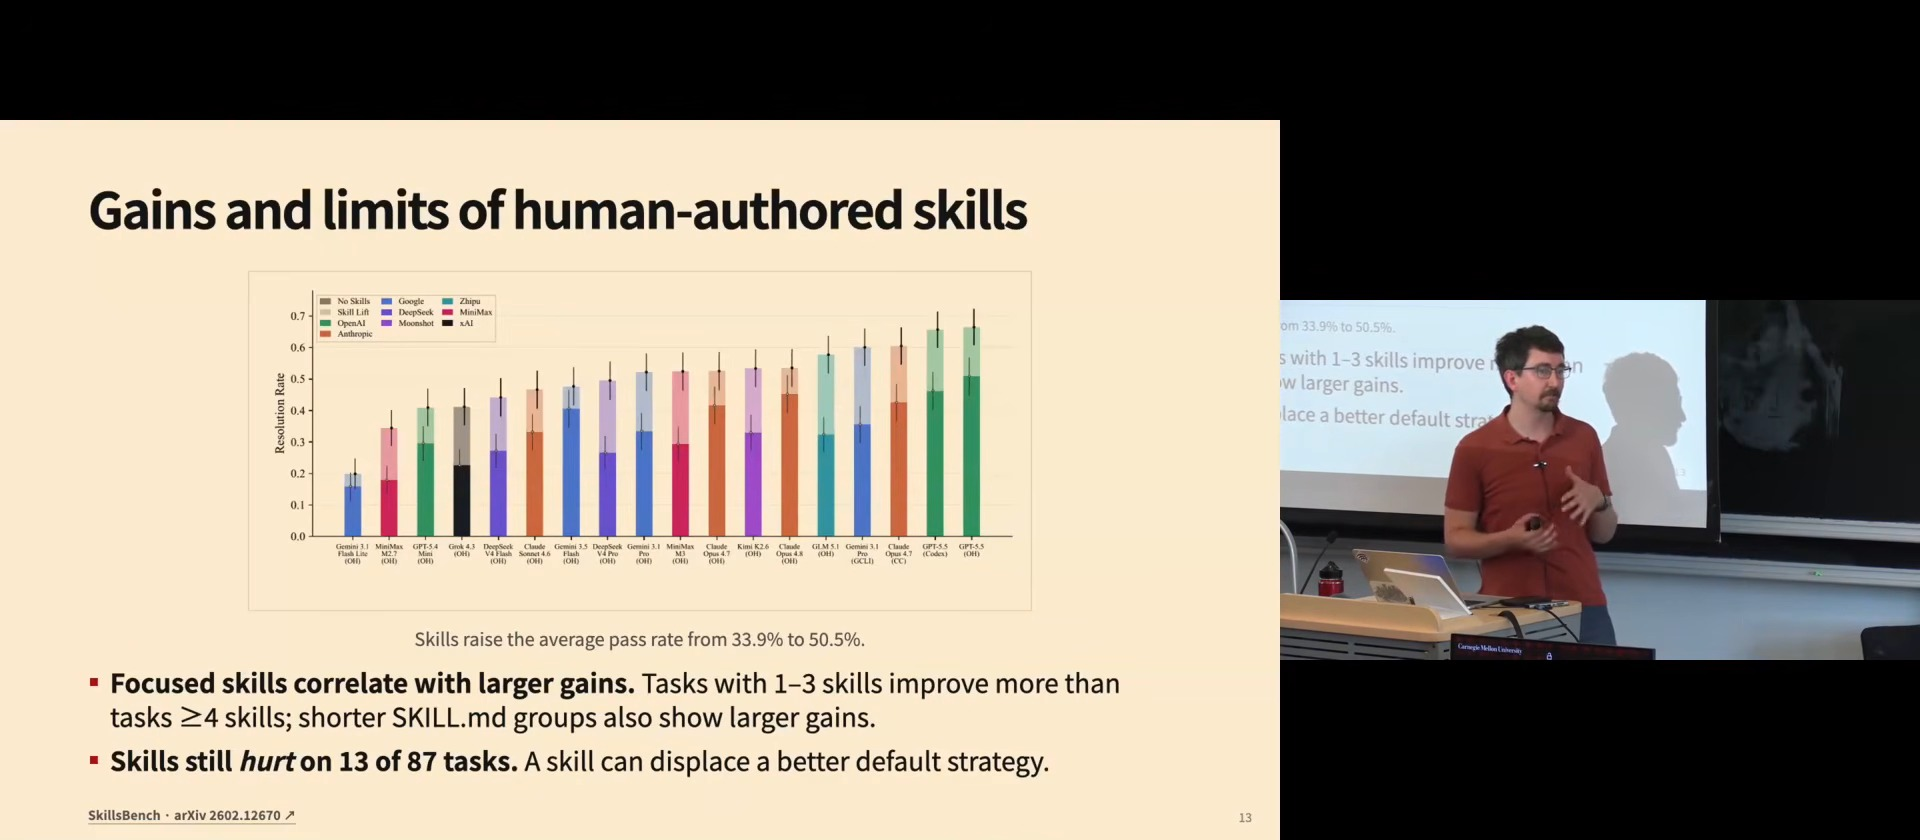
\includegraphics[width=\textwidth]{figures/fig_10_skillsbench_gains.jpg}
\caption{人工技能带来的平均通过率提升（从 33.9 到 50.5）与适用边界：任务所需技能越少、SKILL.md 越短，增益越大\vtag}

\end{figure}
\srcnote{00:29:15--00:29:30}

更重要的是，技能在 87 个任务中的 13 个上仍然有害：一个技能可能挤掉本来更好的默认策略。视频据此把“检查技能是否真的让输出变好”列为使用技能的前提，而不是可选项。

\begin{importantbox}{收益随难度递减这一现象有两种解释}
任务需要的技能越多，往往也越难，收益本来就会被难度摊薄；但视频同时提醒另一种可能：可用技能越多，模型越容易被无关内容带偏。评测本身无法完全区分这两者，但它们指向不同的改进方向。前者是任务性质，后者可以通过更好的检索或更强的模型来缓解。
\end{importantbox}

\subsection{技能从哪里来}

技能包有三种来源，如图~图 11 所示。它可以是随智能体框架一起发布的默认技能；可以由人写好后提交到仓库的 .agents/skills/ 目录，或从其他仓库与注册表安装；也可以由智能体自己创建。后一类里，一些框架提供了 skill\_manage 之类的工具来新建、修改或删除技能，另一些框架提供 skill-creator 命令，把刚完成的工作流草拟成技能包，再由人复核后发布。视频转述的实践建议是：不要凭空从零写技能，而是在刚做完一次工作流之后立刻生成它。

\begin{figure}[H]
\centering
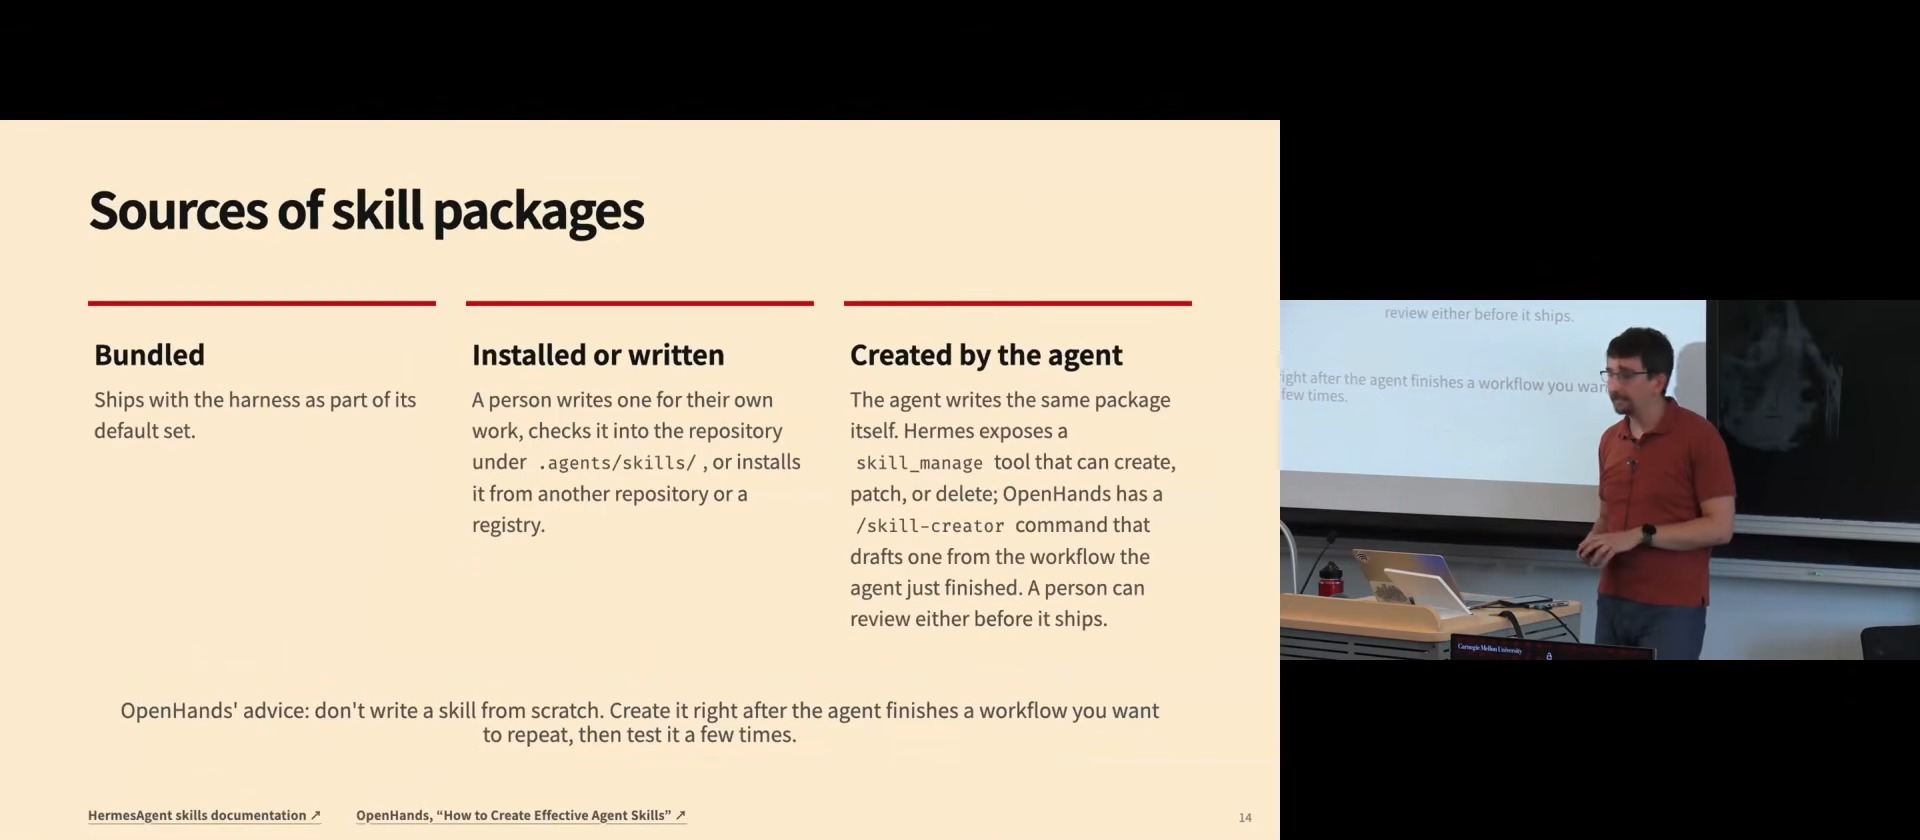
\includegraphics[width=\textwidth]{figures/fig_11_skill_sources.jpg}
\caption{技能包的三种来源：随框架捆绑的默认集、人工安装或写入仓库、以及智能体在完成工作流后自建\vtag}

\end{figure}
\srcnote{00:29:30--00:29:45}

\subsection{维护闭环：让技能随使用改进}

技能写出来只是开始。视频给出了一个具体的维护案例：OpenHands 在自己的仓库里对每个拉取请求运行审查技能，并记录每一次运行；当拉取请求合并后，用一个模型裁判统计智能体提出的建议有多少被人采纳，从而给这次运行打分；再由模型阅读运行记录，找出反复出现的失败模式。图~图 12 把这条闭环画成四个环节：运行技能、记录每次运行、打分、找出复发失败、改写 SKILL.md。案例中反复出现的两类失败是忽略仓库约定（约 15\%）和批准带有严重缺陷的拉取请求（约 10\%）。

\begin{figure}[H]
\centering
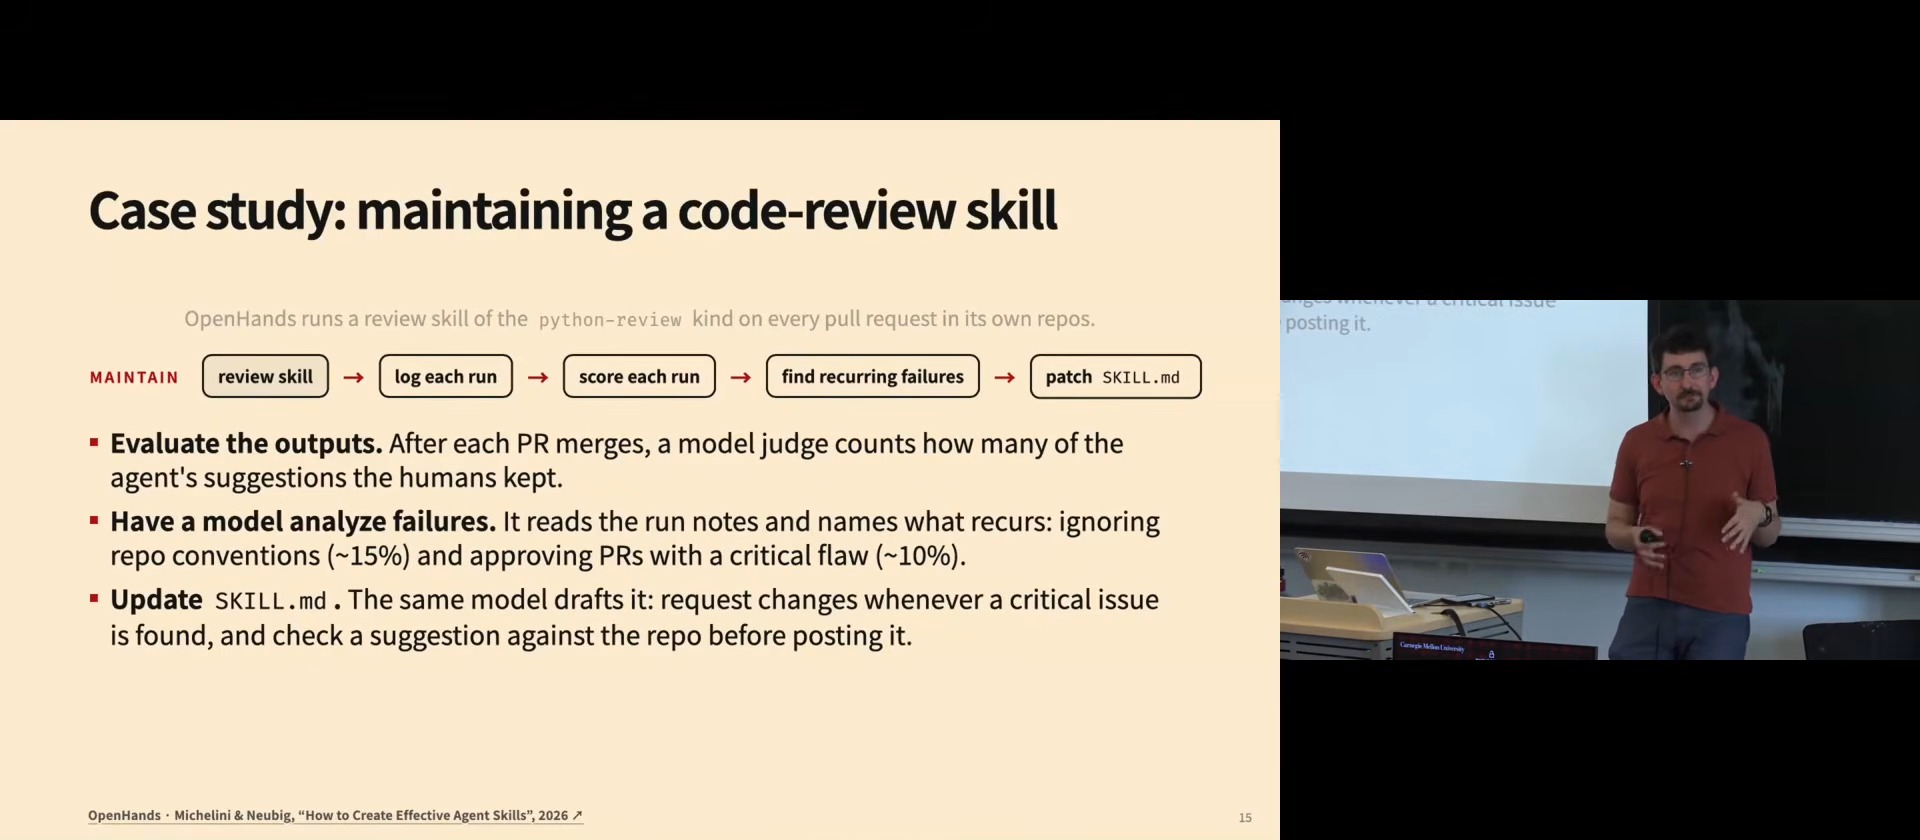
\includegraphics[width=\textwidth]{figures/fig_12_code_review_maintain.jpg}
\caption{代码审查技能的维护闭环：运行、记录、评分、找出复发失败并改写 SKILL.md；案例中忽略仓库约定约占 15\%，批准带严重缺陷的请求约占 10\%\vtag}

\end{figure}
\srcnote{00:32:00--00:32:15}

这条闭环把技能维护变成了一个可测量的过程：先定义一个可观测的指标（建议被采纳的比例），再让模型从大量样本中总结失败模式，最后把结论写回技能文本。它也解释了为什么技能应该基于真实交互而不是凭空设想：只有在真实任务中，才会暴露出“哪些建议对人真正有用”这类事先无法预判的信息。

\subsection{本章小结}

评测给出了两点结论。技能在受控条件下确实带来平均增益，但增益随任务复杂度下降，而且在少数任务上有害。因此技能不是写完就结束的资产，而是一个需要持续评测和改写的对象。下一节转向外部记忆本身的机制：记忆如何被写入、检索，以及当新旧信息冲突时如何更新。

\section{外部记忆的机制：MemGPT 与冲突更新}

\subsection{MemGPT：把记忆分成层级}

MemGPT 是 2023 年的工作，也是最早把外部记忆管理引入语言模型系统的一批论文之一。它的思路借用操作系统里的存储层级：模型能直接读写的上下文窗口是快而小的那一层，窗口之外则是大而慢的归档与回忆存储。图~图 13 给出了这套结构：固定的系统指令、可读写的工作上下文、输出缓冲、队列管理器与函数执行器，以及归档存储和回忆存储。

\begin{figure}[H]
\centering
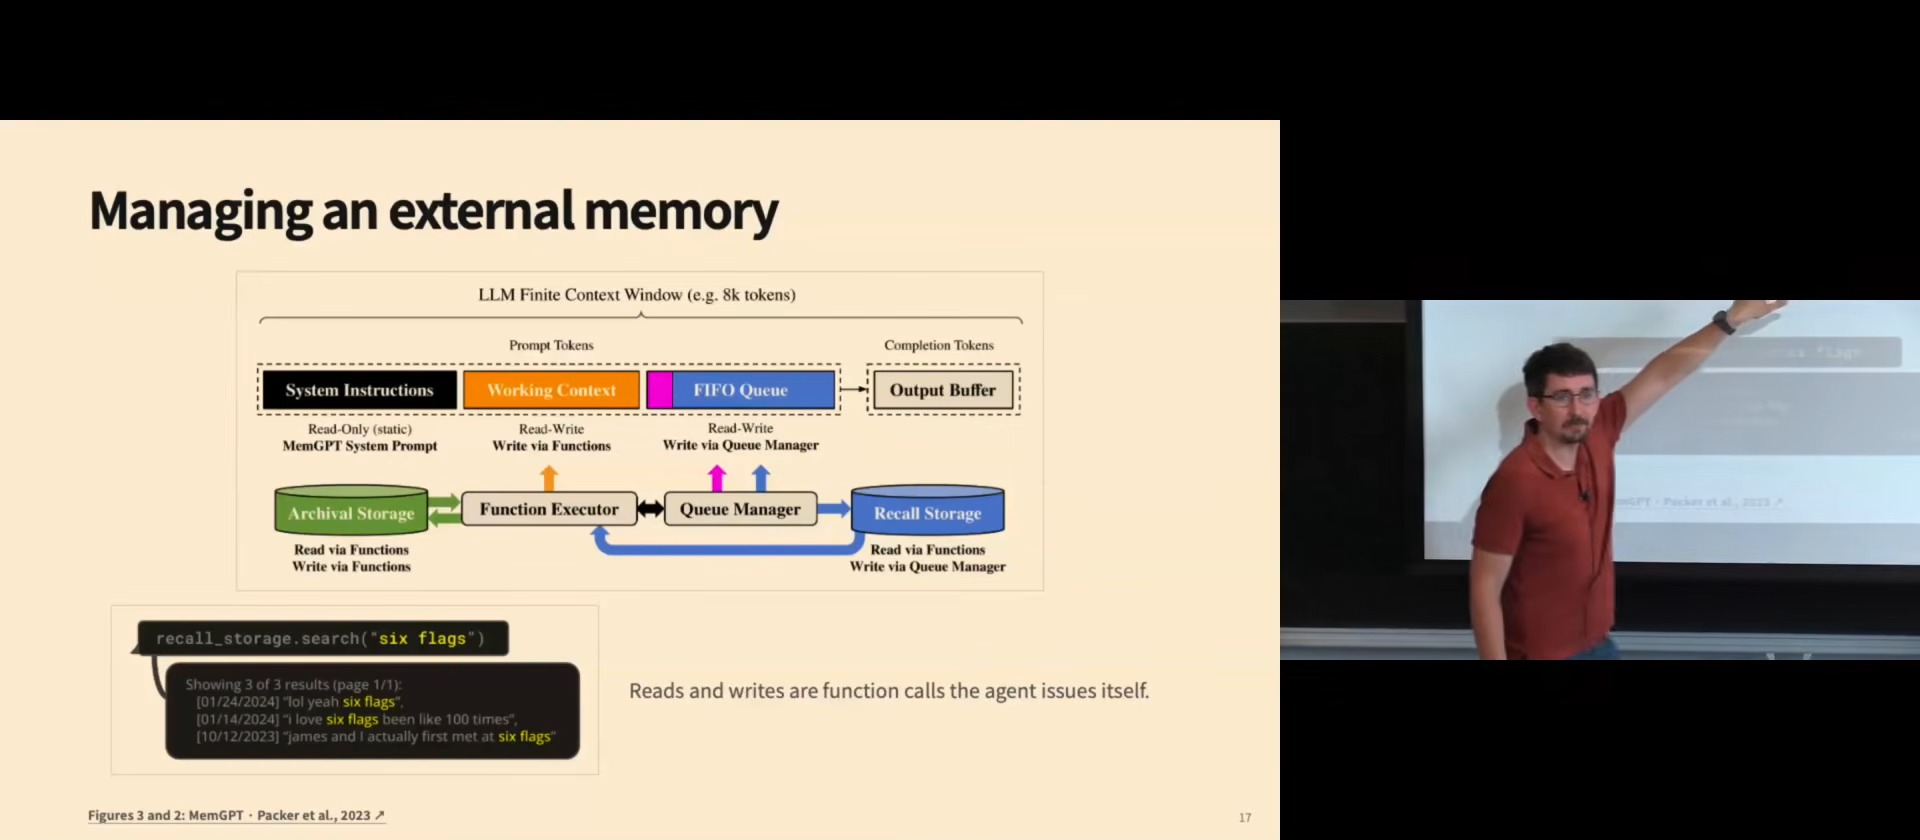
\includegraphics[width=\textwidth]{figures/fig_13_memgpt_memory.jpg}
\caption{MemGPT 式外部记忆：系统指令只读，工作上下文可读写，归档与回忆存储通过工具调用读取，并支持写回\vtag}

\end{figure}
\srcnote{00:34:45--00:35:00}

这套设计在原文写作时很有说服力，因为当时的上下文窗口大约只有 8,000 token。今天窗口已经可以到 1,000,000 token 量级，但视频指出，想放进去的内容增长得更快，因此分层记忆对智能体仍然成立。视频举的例子是：用户提到 Six Flags，系统调用回忆存储的搜索工具，把过去提到过 Six Flags 的记录取回并放进工作上下文，模型随即可以使用这些内容。读和写都由工具调用触发，这一点与上一节技能的渐进披露是同一种思路。

\subsection{冲突更新：ADD、UPDATE、DELETE 与 NOOP}

只追加的记忆会遇到现实问题：用户说“我在某公司工作”，后来说“我被裁员了”，旧事实就不再成立。视频介绍的后续工作给记忆加上了更新机制。图~图 14 把流程分成两个阶段：抽取阶段读入最近若干条消息，由语言模型抽出一组候选记忆；更新阶段先用嵌入检索取出数据库中与候选最相似的若干条记忆，再让语言模型对每一条候选做出决策。

\begin{figure}[H]
\centering
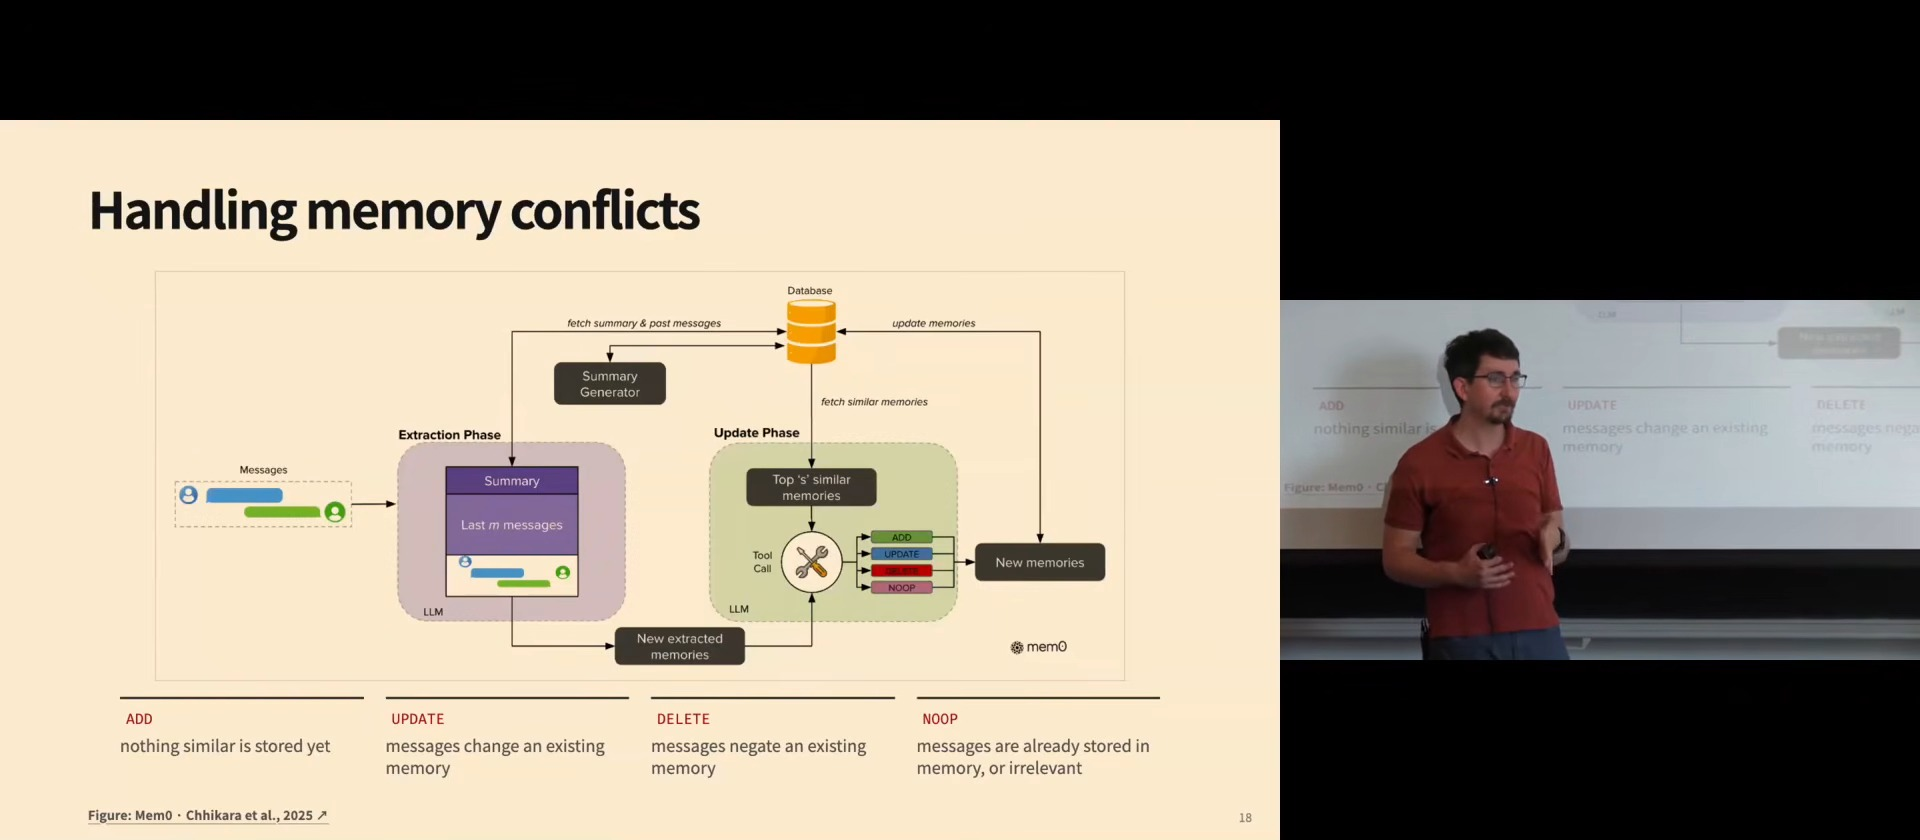
\includegraphics[width=\textwidth]{figures/fig_14_memory_conflicts.jpg}
\caption{记忆冲突处理：抽取阶段生成候选记忆，更新阶段检索相似记忆并做出 ADD、UPDATE、DELETE 或 NOOP 决策\vtag}

\end{figure}
\srcnote{00:36:45--00:37:00}

四种决策的含义在图中直接标出：候选与已有记忆都不相似时执行 ADD；候选改变了某条已有记忆时执行 UPDATE；候选否定了某条记忆时执行 DELETE；候选已经存在或与任务无关时执行 NOOP。本讲义把这一决策压缩成一个记号：

\[
m_{\text{new}} = f_{\text{LLM}}(m_{\text{cand}},\; R_k(m_{\text{cand}})),
\qquad
m_{\text{new}} \in \{\text{ADD}, \text{UPDATE}, \text{DELETE}, \text{NOOP}\}.
\]

\begin{itemize}
\item $m_{\text{cand}}$：从最近消息中抽取出的候选记忆；
\item $R_k(m_{\text{cand}})$：按嵌入相似度检索出的前 $k$ 条已有记忆；
\item $f_{\text{LLM}}$：由语言模型执行的冲突判定；
\item $m_{\text{new}}$：最终采取的更新动作。
\end{itemize}

这套“检索相关项、再改写它”的模式与线性注意力里的 Delta 类方法同构：先按查询取出已存的值，再修改它们，而不是只做追加。视频在问答中明确点出了这层类比，也提到权重层面的更新同样需要“遗忘”机制，例如机器遗忘研究。

\begin{knowledgebox}{为什么“能删”和“能改”很重要}
只追加的记忆会积累过期信息，而且过期信息与最新信息同时被检索到时，模型无法判断哪个更可信。允许更新和删除，实际上是在维护记忆的一致性，而不只是控制它的容量。视频也坦言，具体的更新细节会随智能体形态而变化，但“允许修改冲突知识”这个原则是通用的。
\end{knowledgebox}

\subsection{本章小结}

MemGPT 给了外部记忆的骨架：分层存储、工具驱动的读写。冲突更新补上了保持一致性的机制：抽取、检索、判定、改写。这两件事都在处理“记忆里放什么”。下一节处理另一半问题：一次尝试的对错如何变成可复用的信号。

\section{从反馈与轨迹中学习}

\subsection{用自然语言反馈条件化下一次尝试}

如果一个任务允许重试，那么第一次失败本身就能提供信息。视频介绍的 Reflexion 把这一点做成了简单而有效的流程：智能体先尝试一次，由一个评估器预测这次尝试的回报；若失败，就生成一段自然语言反馈，说明哪里做错了；然后带着这段反馈重试同一个任务。图~图 15 给出了论文里的例子：问题是 1776 年 10 月 28 日发生在 White Plains 附近的一系列战斗，智能体第一次只答出了单场战斗的名称；模型生成的反馈指出“问题问的是一系列战斗，而我只给出了一场”，第二次尝试因此答对。

\begin{figure}[H]
\centering
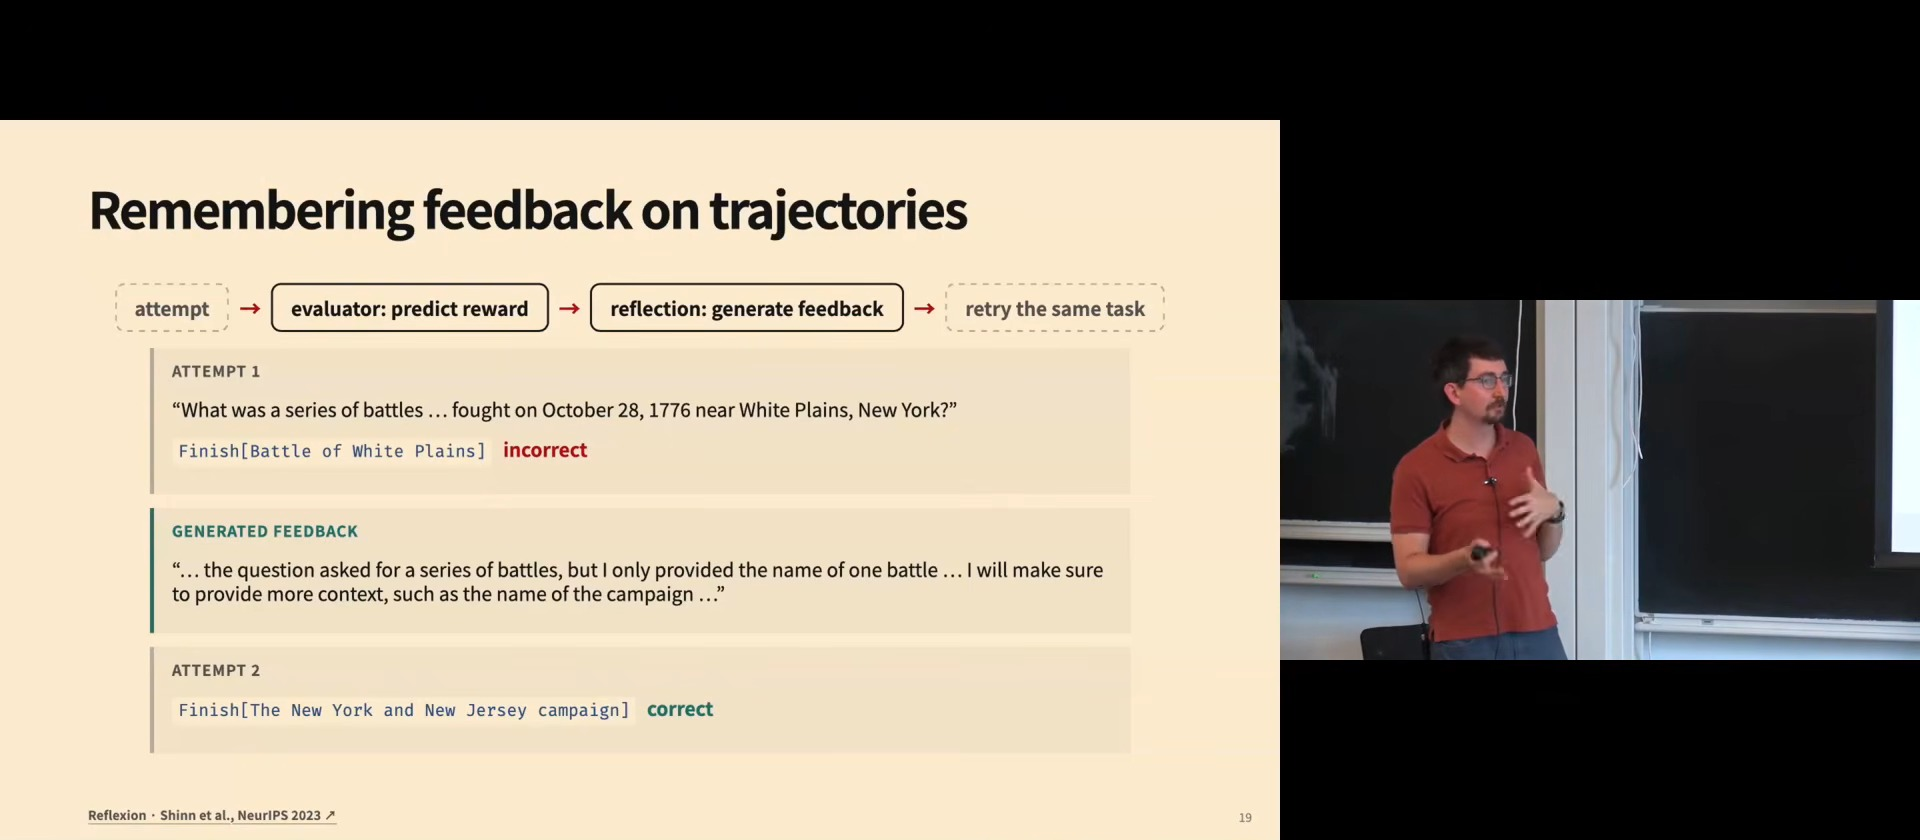
\includegraphics[width=\textwidth]{figures/fig_15_reflexion_feedback.jpg}
\caption{Reflexion 流程：尝试、评估回报、反思生成自然语言反馈、重试同一任务；图中给出问题、错误答案与生成的反馈\vtag}

\end{figure}
\srcnote{00:41:00--00:41:15}

这段反馈的价值在于它是一句可读的“诊断”，而不是一个分数。模型可以把它当作条件，在第二次尝试时避开同样的错误。视频进一步指出，这种反馈不限于同一个任务：只要反馈足够一般化，它也能帮助解决相似的任务。

\subsection{相似轨迹条件化}

比单条反馈更激进的方案是保存整条轨迹。视频把这一类方法概括成“相似轨迹条件化”：准备一个经验池，把过去任务的完整轨迹存进去，包括成功与失败；新任务到来时，按任务描述检索出最相关的轨迹，把它放进上下文作为参考。图~图 16 展示了这个过程，并列出经验池的三种来源：离线训练阶段收集、智能体工作过程中逐步累积，或者由人手写。存储时轨迹有时会被改写和标注。

\begin{figure}[H]
\centering
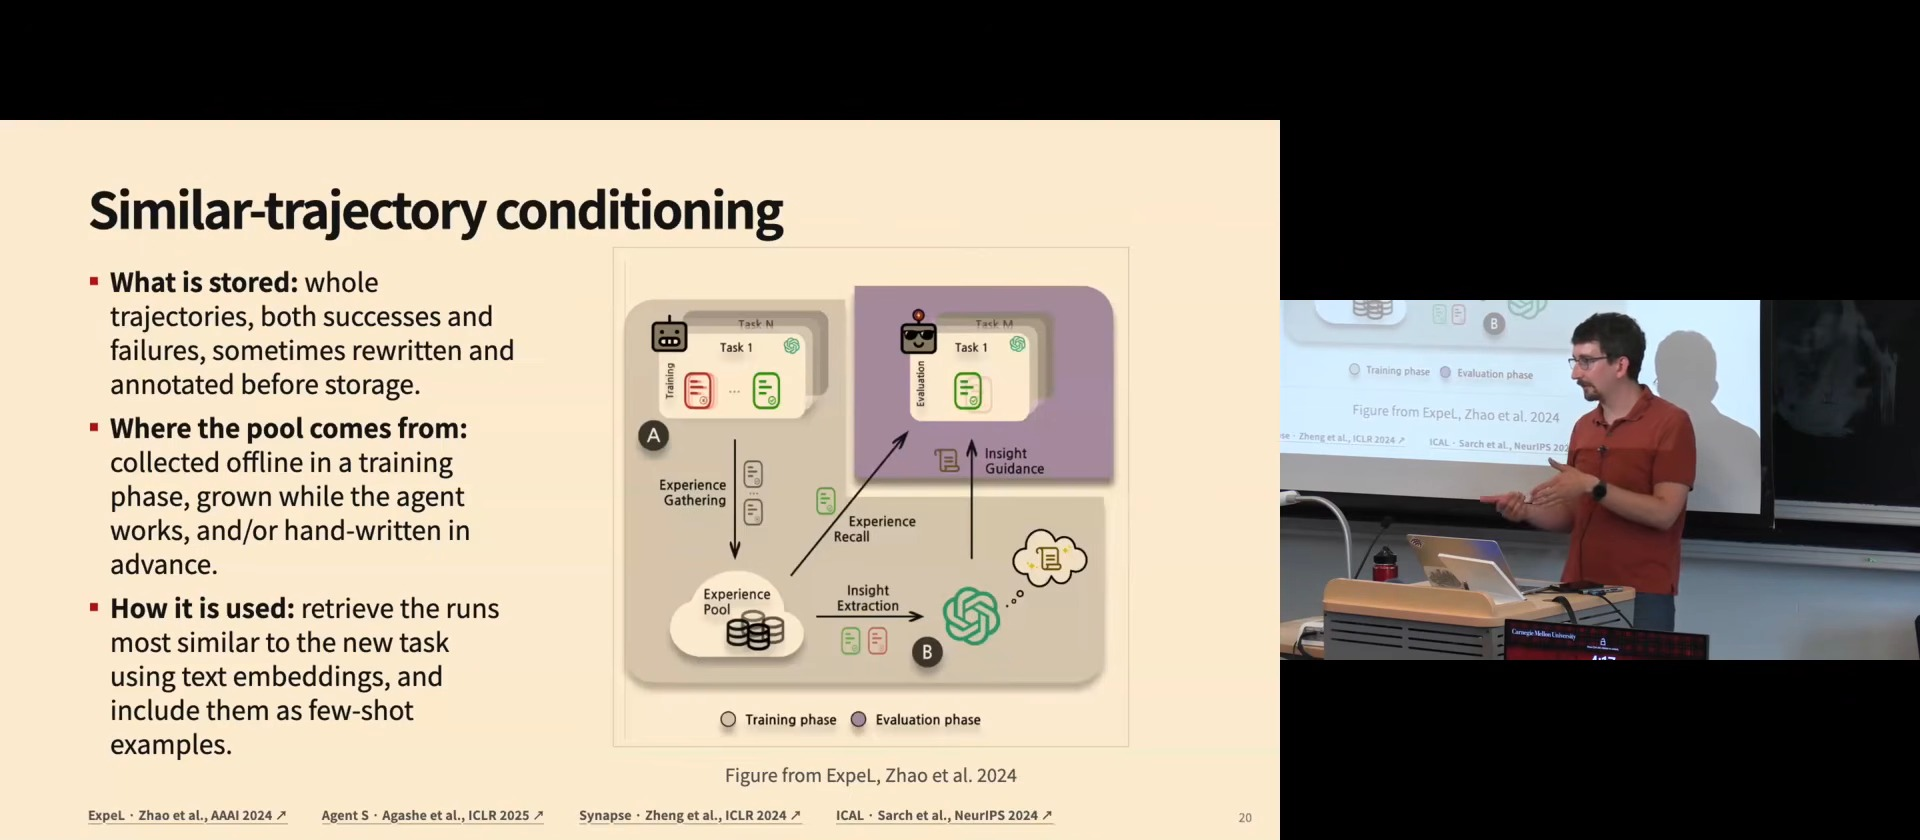
\includegraphics[width=\textwidth]{figures/fig_16_trajectory_conditioning.jpg}
\caption{相似轨迹条件化：把成功与失败的整条轨迹存入经验池，按任务描述召回后放进上下文；经验池可离线收集、在线累积或人工写入\vtag}

\end{figure}
\srcnote{00:43:30--00:43:45}

视频借这个例子定义了“轨迹”：在一次任务中，智能体从环境或用户收到的观察、它发出的工具调用，以及它产生的思维链，按顺序组成的消息序列。检索通常是把新任务的文本描述做嵌入，和池中每个任务的描述比较；也可以加一层领域约束，只召回同一领域下的轨迹。

\begin{knowledgebox}{反思有效的前提是反馈足够一般}
反馈如果只描述这一次的具体错误，就只能改善同一个任务；只有把教训提升成可迁移的规则，才能帮助相似任务。视频用“问一系列战斗却只答出一场”的例子展示了这条界线：有效的反馈说的是“答案的范围错了”，而不是“这个字符串应换成另一个字符串”。
\end{knowledgebox}

\begin{warningbox}{轨迹越长越贵，也越难迁移}
保存整条轨迹意味着保真度最高，但也意味着上下文开销最大，而且轨迹里大量细节是与原任务绑定的，迁移到新任务时未必有用。视频把“哪些部分可复用”这个问题留给下一节：与其存整条轨迹，不如先把可复用的片段抽象出来。
\end{warningbox}

\subsection{本章小结}

反馈把一次失败转成一句诊断，轨迹则把整段经历变成可召回的样本。两者都在扩大模型可以条件化的信息。但整条轨迹太粗，下一节讨论如何从轨迹中提取出更抽象、更容易复用的技能。

\section{从经验中归纳技能}

\subsection{技能是可复用的任务片段}

图~图 17 把上一节的共享结构落到具体动作上。搜索商品时，智能体先向搜索框填入查询，再点击搜索按钮；报告价格区间时，前半段完全相同，只是之后多了一步读取最低价与最高价。可复用的正是“搜索”这一段，后半段是任务专属的增量。视频由此提出一个判断：技能就是任务中被复用的那一段，问题是该用什么形式表示它。

\begin{figure}[H]
\centering
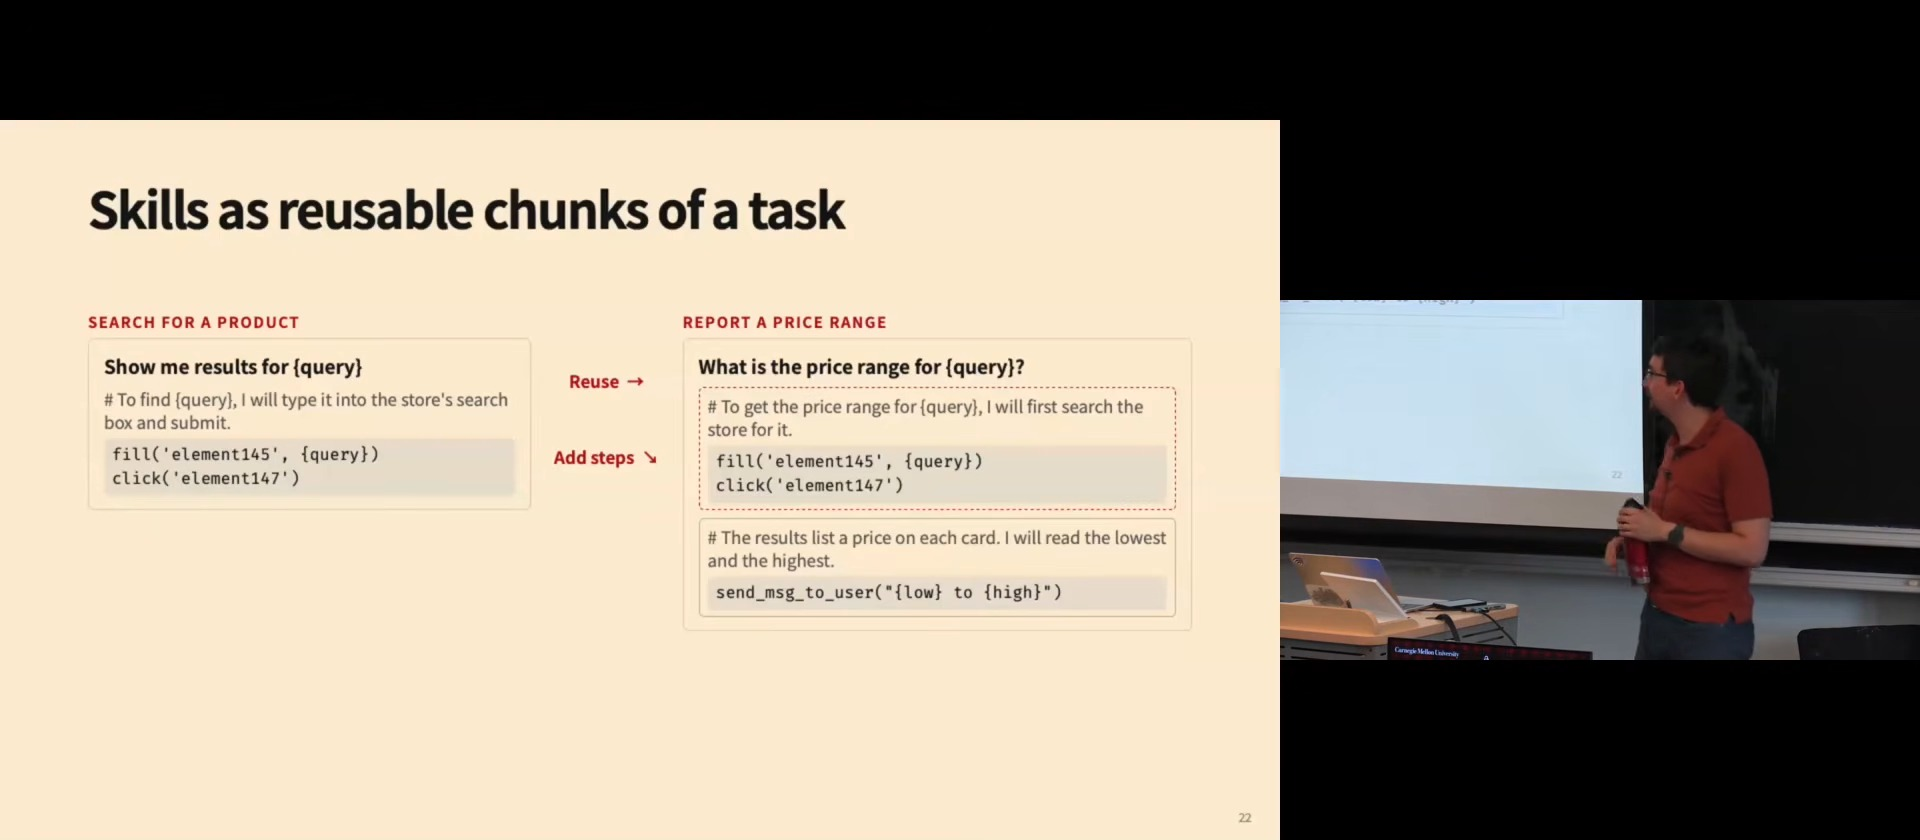
\includegraphics[width=\textwidth]{figures/fig_17_skill_reusable_chunks.jpg}
\caption{技能是可复用的任务片段：搜索商品与报告价格区间共享同一段填入查询并提交的动作，后者只多出读取价格的步骤\vtag}

\end{figure}
\srcnote{00:46:00--00:46:15}

直接照搬具体动作会有一个明显弱点。如果技能记下的是“点击编号为 element145 的控件”，那么页面元素编号一变，技能就失效；换一家搜索界面不同的网站，技能同样失效。视频在问答里给出了这个反例，并说明后续讲次会用不同的动作空间来缓解元素编号问题，但跨站点的失效需要另一种机制。

\subsection{早期工作：代码技能库与函数抽取}

技能归纳并不是大模型时代才有的想法。视频回顾了两条前史。第一条是 Voyager，它让智能体在 Minecraft 里用代码控制角色：把“合成某件物品”“击败僵尸”这类子任务写成函数，函数可以调用更早学会的函数，因此技能库能组合出越来越复杂的行为。第二条来自程序归纳社区，以 DreamCoder 为代表：从一组由底层函数构造出的完整程序里搜索反复出现的模式，把模式抽象成新函数，再反复压缩整个程序库。图~图 18 把两条线索并置在一起。

\begin{figure}[H]
\centering
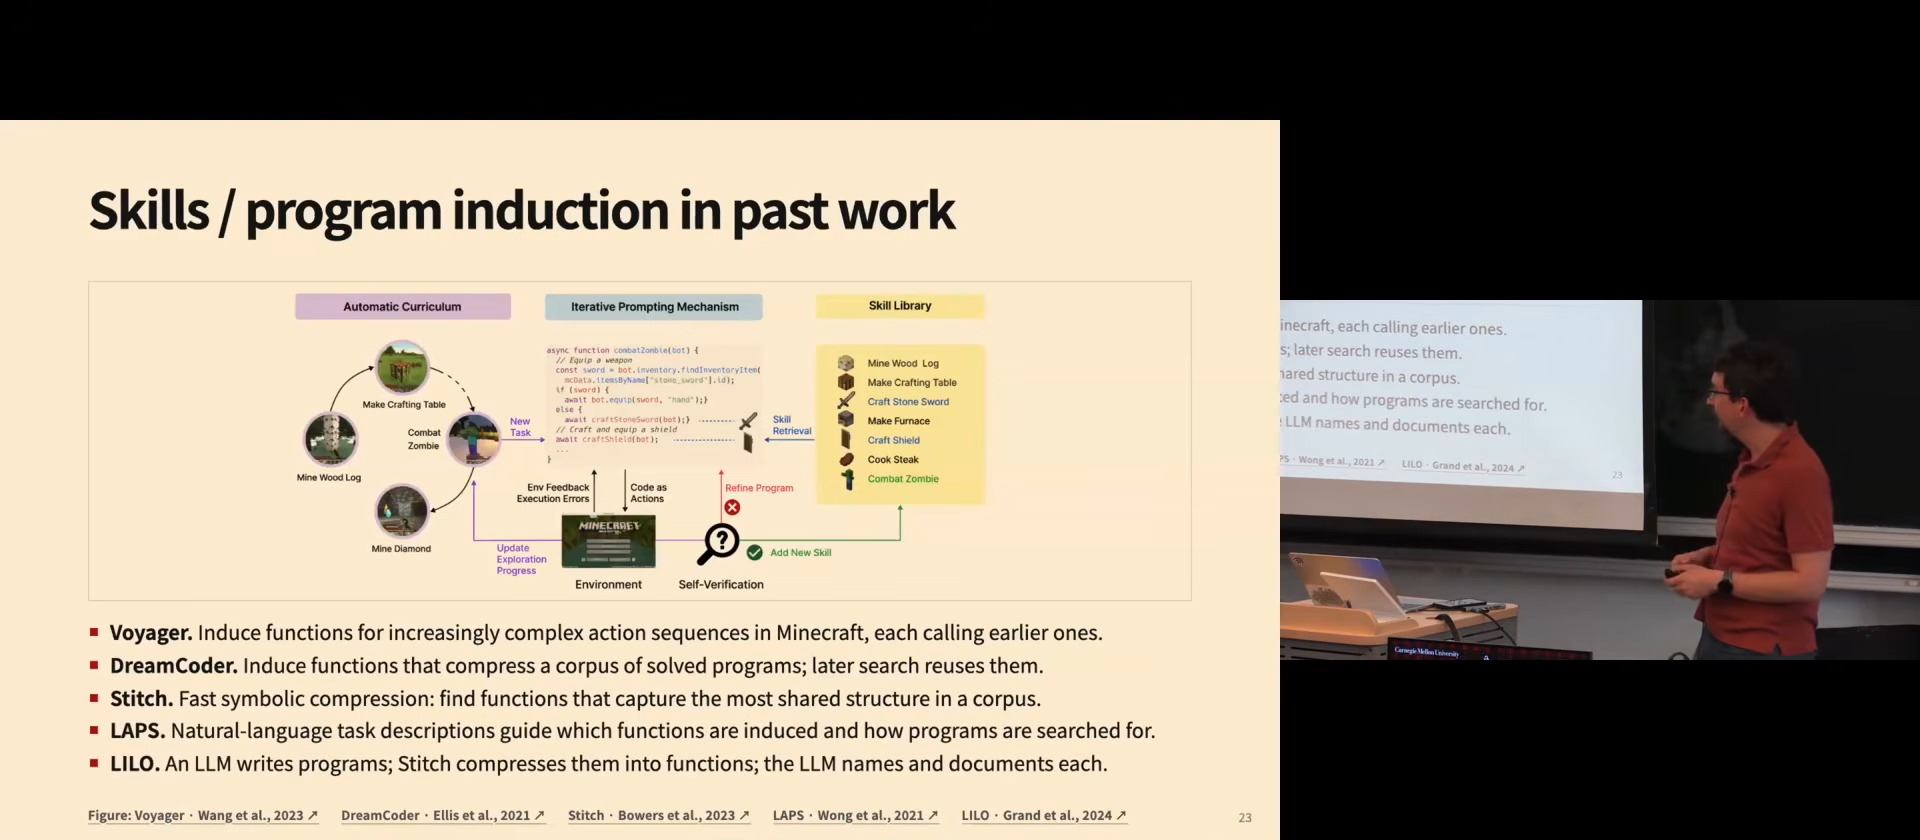
\includegraphics[width=\textwidth]{figures/fig_18_program_induction.jpg}
\caption{早期技能与程序归纳：Voyager 用可相互调用的代码函数组成技能库，DreamCoder 从语料中反复抽取并压缩程序结构\vtag}

\end{figure}
\srcnote{00:48:00--00:48:15}

这两条前史共同说明了一件事：技能库的价值不只在于少写几步，更在于\textbf{组合}。一旦子过程有了名字和接口，它就能被更大的子过程调用。

\subsection{在线评测设定与技能生命周期}

技能归纳的效果通常在在线设定下评测：任务一个接一个到达，智能体在完成每个任务后有机会更新技能记忆，然后带着更新后的记忆去做下一个任务。评价指标是所有已见任务上的累积成功率。图~图 19 画出了这个循环：任务依次到达，成功之后把归纳出的技能写入记忆，记忆随着评测流不断增长，并在后续任务上被应用。

\begin{figure}[H]
\centering
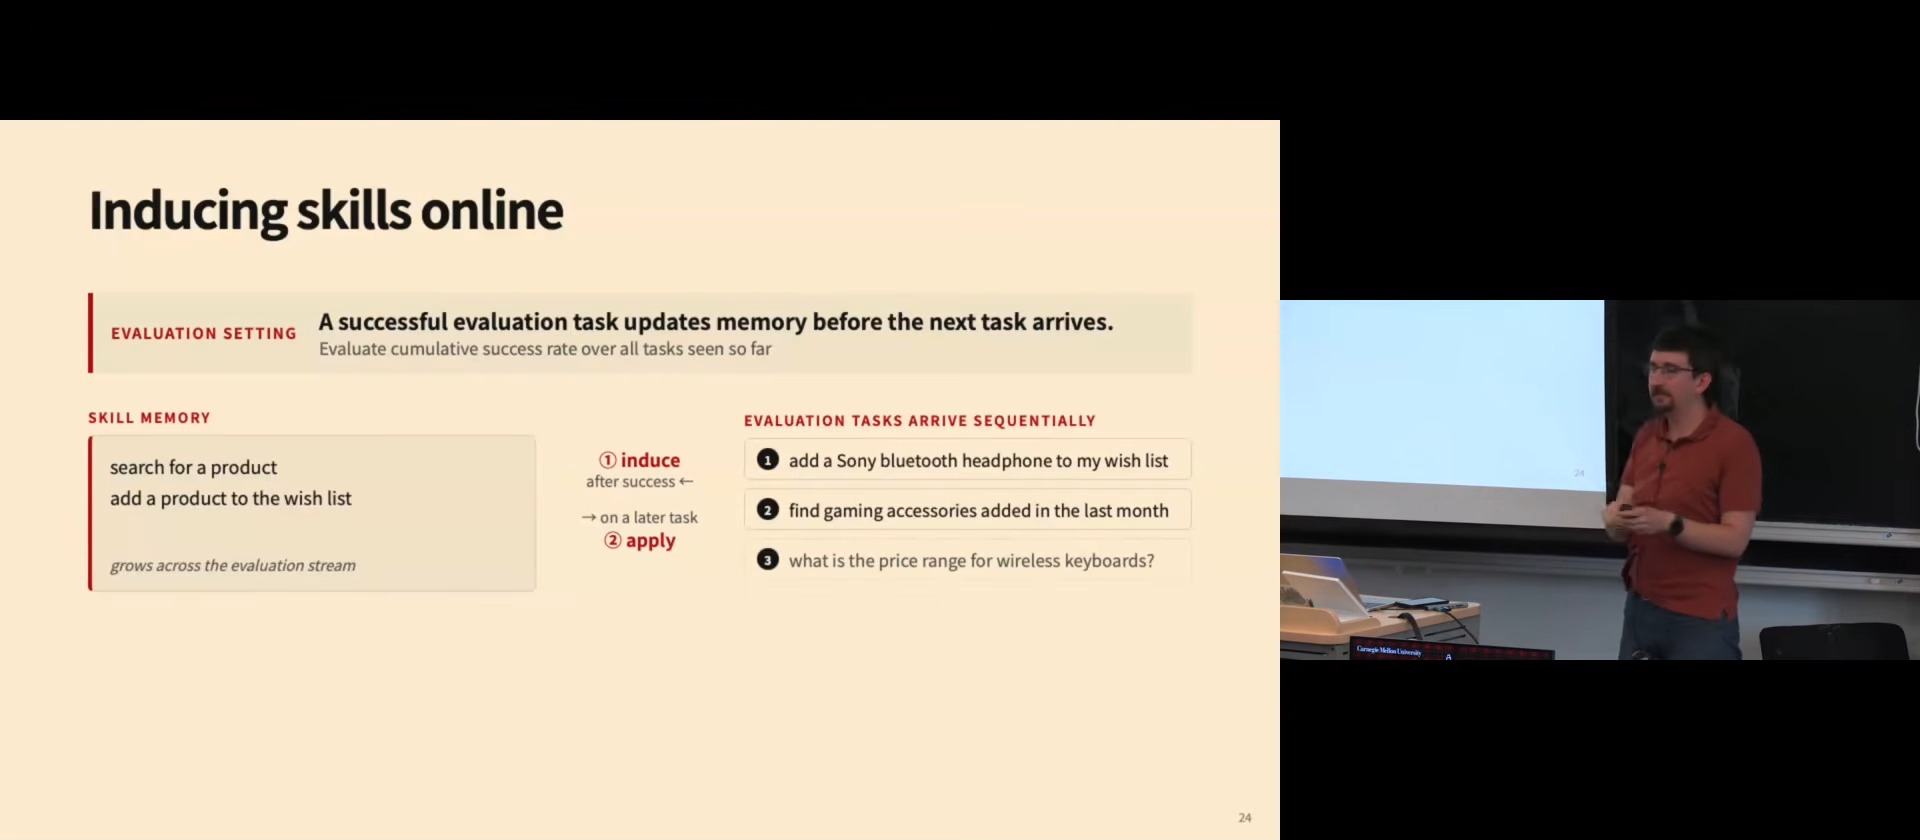
\includegraphics[width=\textwidth]{figures/fig_19_online_induction.jpg}
\caption{在线技能归纳设定：任务依次到达，成功即把技能写入记忆，记忆随评测流增长并在后续任务上复用\vtag}

\end{figure}
\srcnote{00:49:45--00:50:00}

若用 $s_i$ 表示第 $i$ 个任务是否成功，则第 $t$ 个任务之后的累积成功率可以写成

\[
\mathrm{SR}_t = \frac{1}{t} \sum_{i=1}^{t} \mathbf{1}[\,s_i = \text{success}\,].
\]

\begin{itemize}
\item $t$：到目前为止已经完成的任务数；
\item $s_i$：第 $i$ 个任务的结果；
\item $\mathbf{1}[\cdot]$：指示函数，条件成立时取 1，否则取 0；
\item $\mathrm{SR}_t$：截至第 $t$ 个任务的累积成功率。
\end{itemize}

这条指标衡量的是“越做越好”这件事本身：如果技能记忆确实有用，曲线应当随任务推进而上升，并且能够覆盖越来越复杂的任务。

技能在记忆里并不是一放不动。图~图 20 把技能的生命周期分成三段。LEARN 段把一次轨迹变成一条记忆：先判定轨迹是否成功，再从中归纳技能，最后决定是否收录。USE 段把记忆真正用起来：检索、选择、行动，并产生新的结果。MAINTAIN 段处理记忆老化：修复有问题的技能，或者淘汰不再使用的技能。

\begin{figure}[H]
\centering
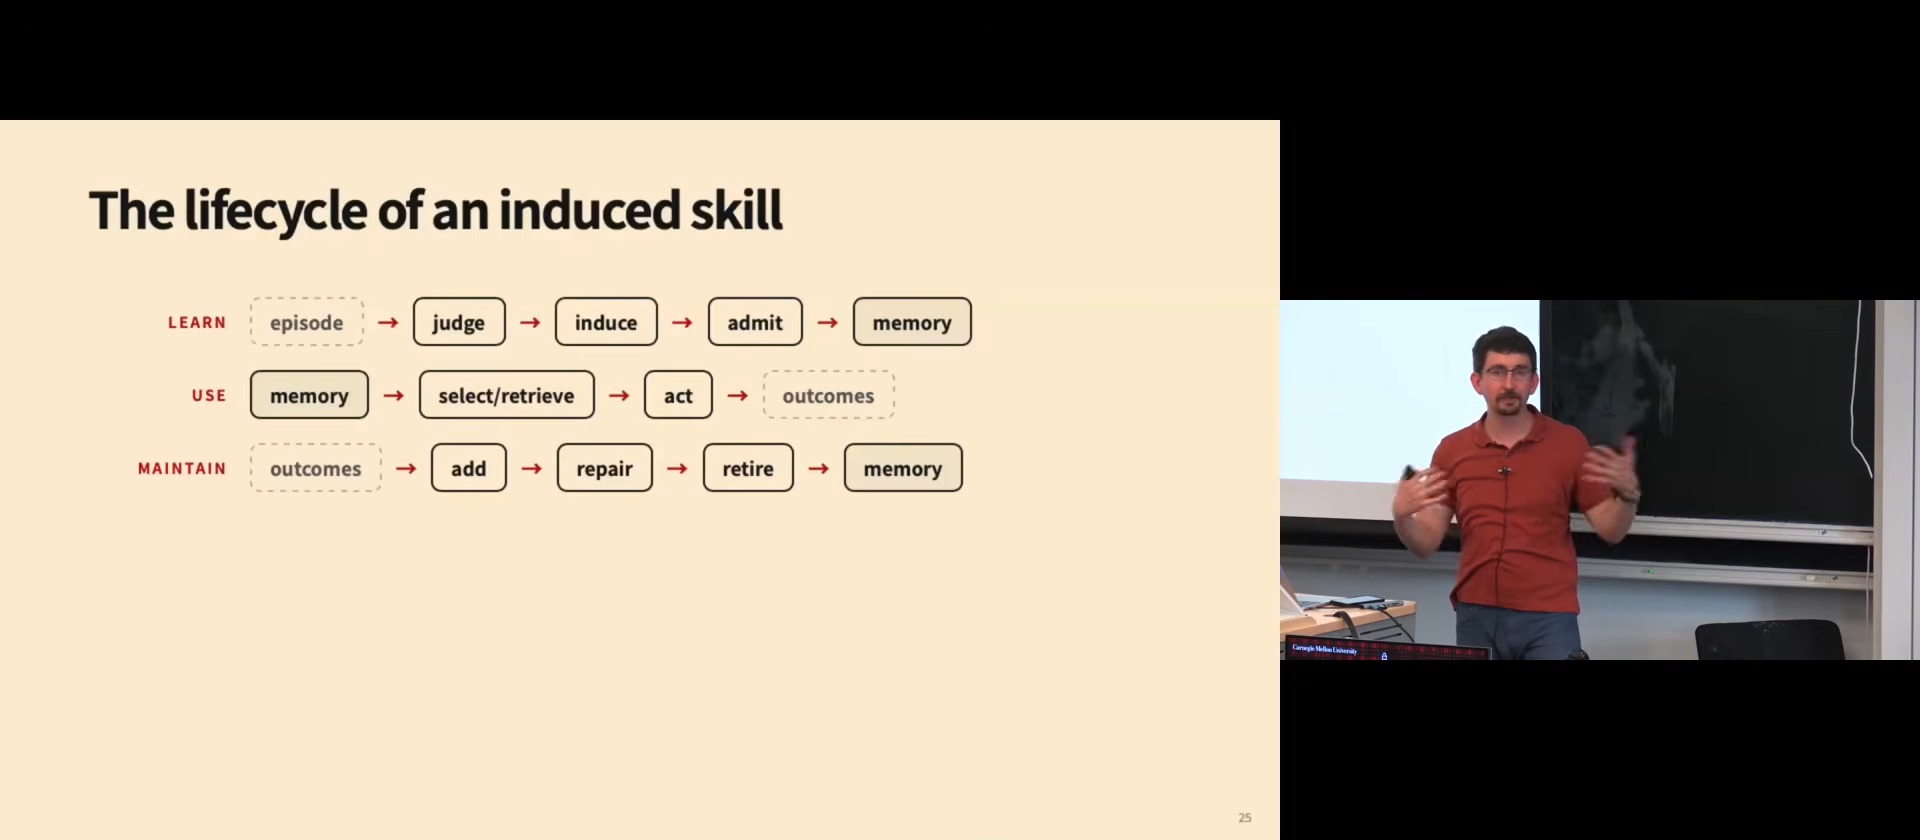
\includegraphics[width=\textwidth]{figures/fig_20_skill_lifecycle.jpg}
\caption{技能生命周期：LEARN 段判定、归纳与收录，USE 段检索与行动，MAINTAIN 段修复与淘汰\vtag}

\end{figure}
\srcnote{00:51:00--00:51:15}

\begin{importantbox}{判定（judge）是收录前的闸门}
在归纳之前先判定轨迹是否成功，是这类系统的共同结构。如果判定给出错误的正例，错误做法就会被写进技能记忆，并在后续任务中被反复使用。视频在后面的消融里专门检验了裁判准确率的影响，这也是为什么维护阶段必须保留删除和修订的入口。
\end{importantbox}

\subsection{本章小结}

技能是任务中被复用的片段，代码技能库和程序归纳给了它形式上的先例。在线设定用累积成功率衡量“越做越好”，而技能生命周期把学习者、使用者和维护者的职责分开。下一节比较两种最主流的表示法：文本技能与代码技能。

\section{文本技能与代码技能}

\subsection{用文本工作流表示技能}

Agent Workflow Memory 是 CMU 的一项工作，做法是把工具调用序列交给语言模型，让它找出其中可能在未来任务中复用的部分，并输出成“工作流”。一条工作流包含两部分：对子任务的描述，以及完成它的动作序列。为了让工作流不只适用于某一个具体查询，模型会把具体参数抽象成模板。图~图 21 给出了一个例子：任务是把商店收到的、提到 satisfied 的评论数报给用户；轨迹包含点击 Marketing、点击 All Reviews、填入 satisfied、点击 Search、把结果 2 发回用户；归纳出的工作流写成“搜索匹配某词条的评论”，动作里用占位符代替具体词条。

\begin{figure}[H]
\centering
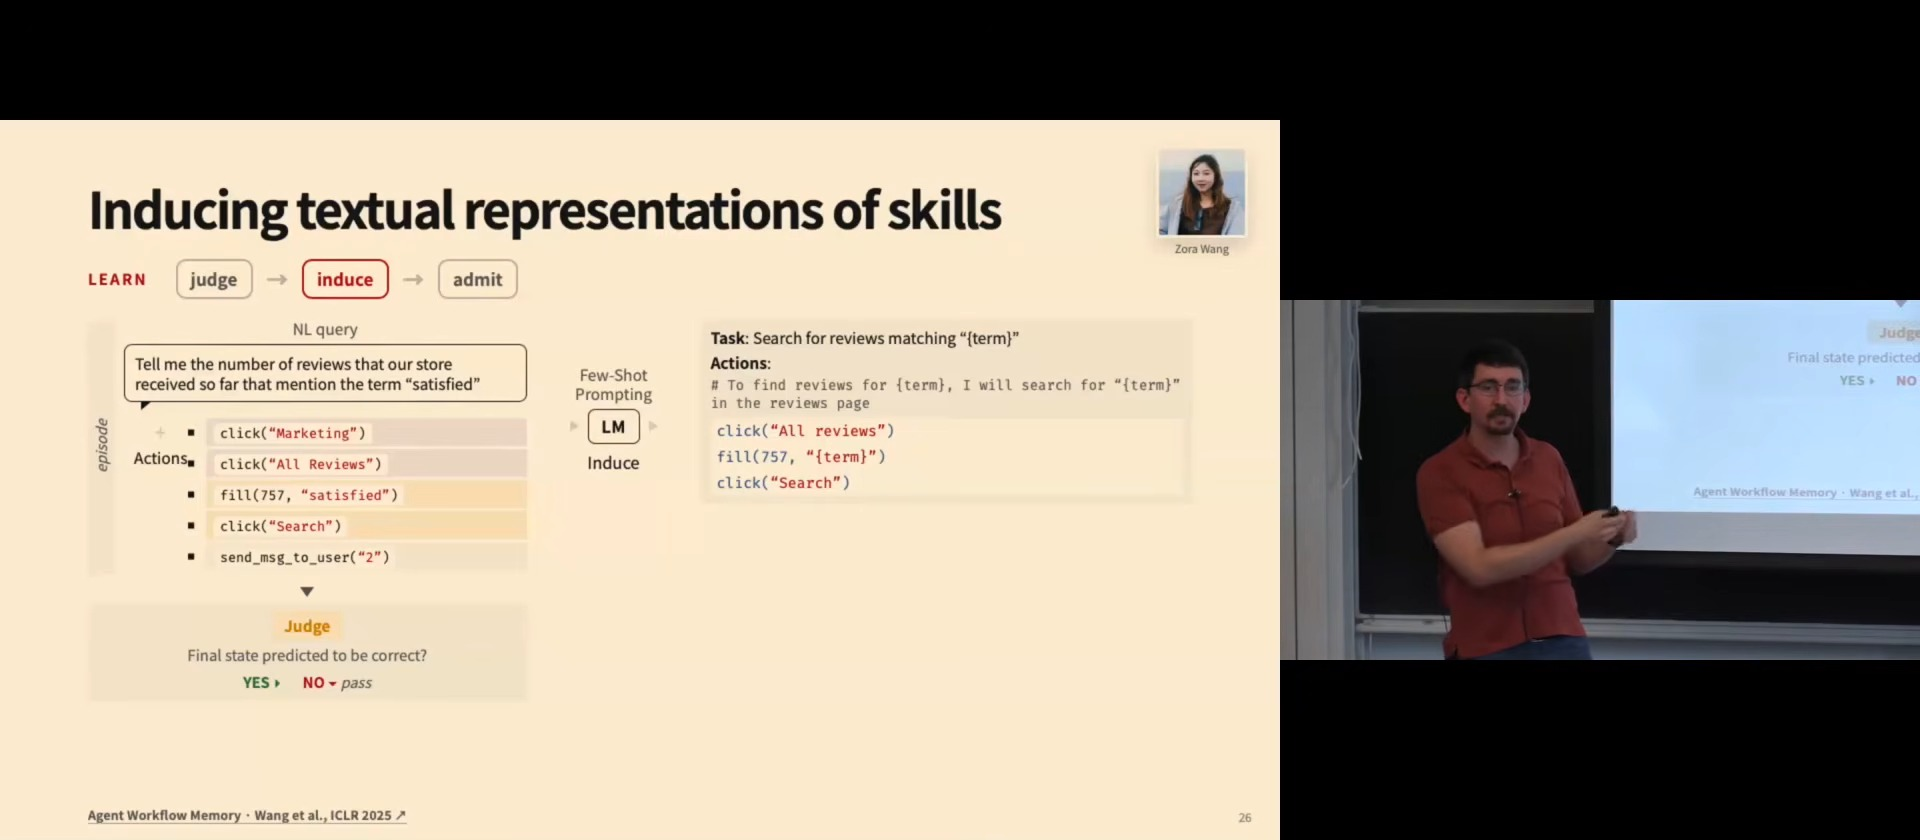
\includegraphics[width=\textwidth]{figures/fig_21_awm_text_workflow.jpg}
\caption{Agent Workflow Memory：把工具调用轨迹归纳成带占位符的文本工作流，先由裁判判定轨迹最终状态是否正确，再决定是否收录\vtag}

\end{figure}
\srcnote{00:52:45--00:53:00}

与前面的做法一致，AWM 也用裁判作为闸门：只有判定轨迹正确的那些工作流才会被写入记忆，因为错误的经验会在未来把模型带偏。使用阶段则把这些工作流放进上下文，具体展示全部内容还是只展示文本描述，取决于技能数量和模型的上下文长度。

视频给出的在线实验结果展示了记忆复利：无记忆的基线在评测流上逐渐收敛到很低的成功率，大致在 10 附近；加入工作流记忆后，两条曲线拉开差距，差距逐渐扩大到约 22.5 个百分点，并且带记忆的智能体能够完成基线做不到的复杂任务，例如找出某地点附近的酒店并给出到附近超市的步行路径。图~图 22 画出了这条曲线和任务难度递增的过程。

\begin{figure}[H]
\centering
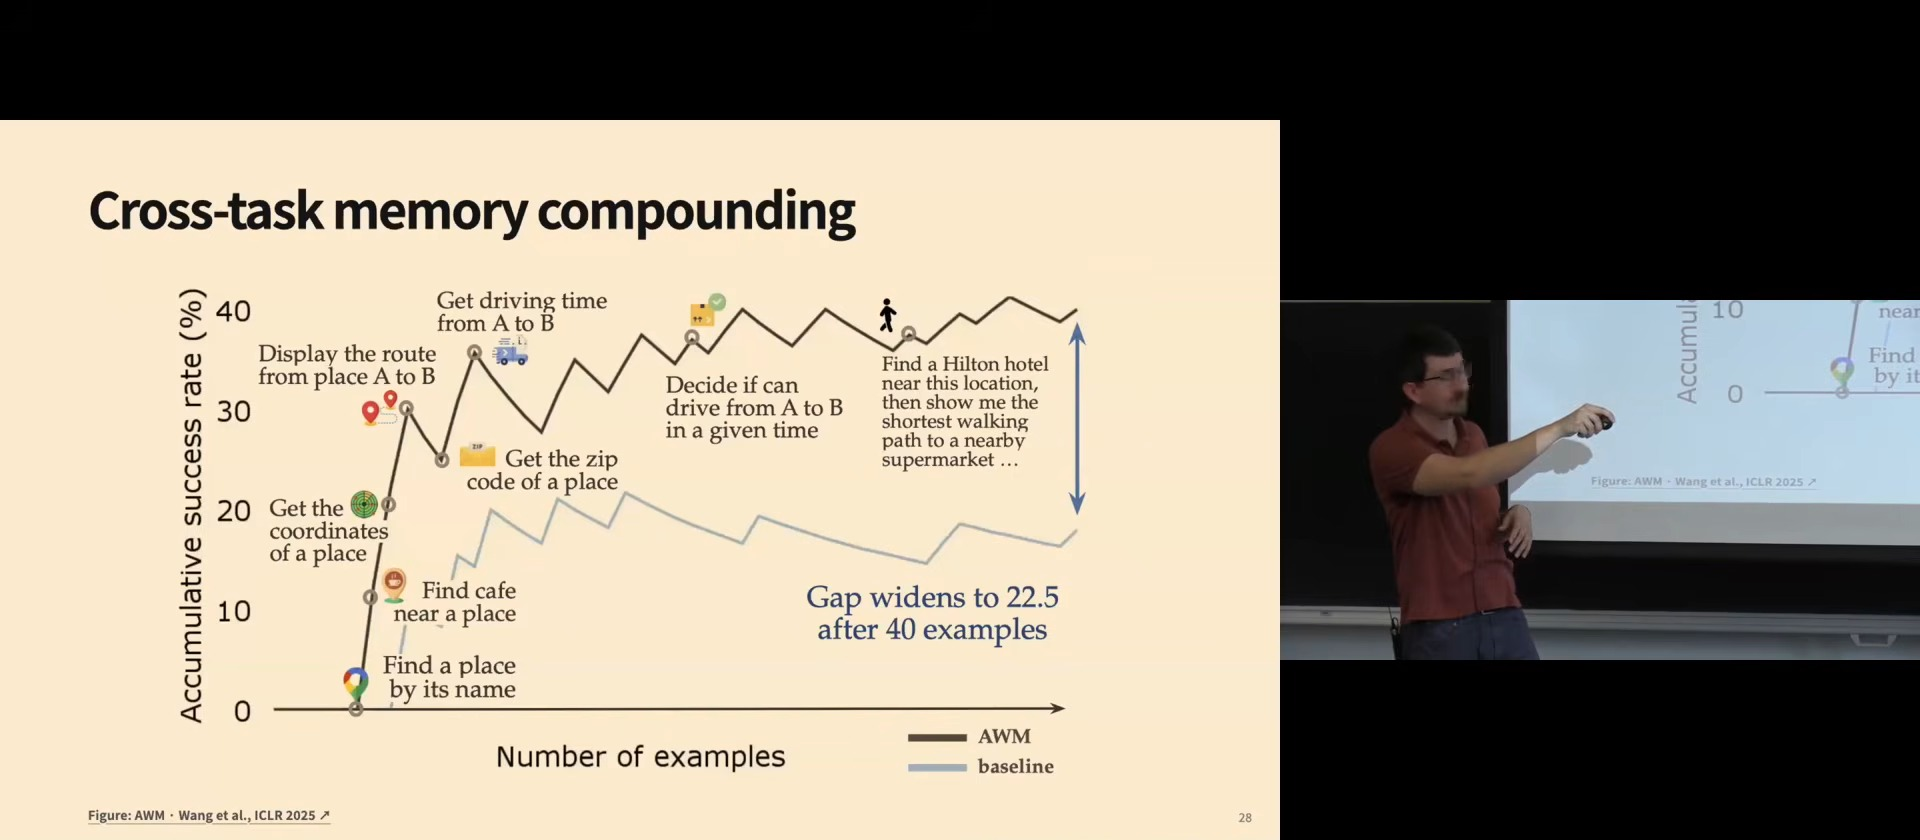
\includegraphics[width=\textwidth]{figures/fig_22_awm_compounding.jpg}
\caption{跨任务记忆复利：带工作流记忆的智能体成功率高于无记忆基线，并在评测流中完成越来越复杂的任务，差距扩大到约 22.5 个百分点\vtag}

\end{figure}
\srcnote{00:54:45--00:55:00}

\subsection{同一段子过程的两种表示}

把同一段搜索子过程表示成文本或代码，差别很具体。文本表示把动作序列和示例轨迹放进上下文，模型在新情境中重新生成每一步工具调用。它灵活：换一个搜索词、换一个控件编号都可以临场调整；代价是每一步都要模型亲自产生，因此慢，而且每次都要重新观察页面。代码表示把这段过程写成一个函数，模型只要以正确参数调用它即可，函数内部的三步动作由环境执行。图~图 23 把两种表示并排放在一起。

\begin{figure}[H]
\centering
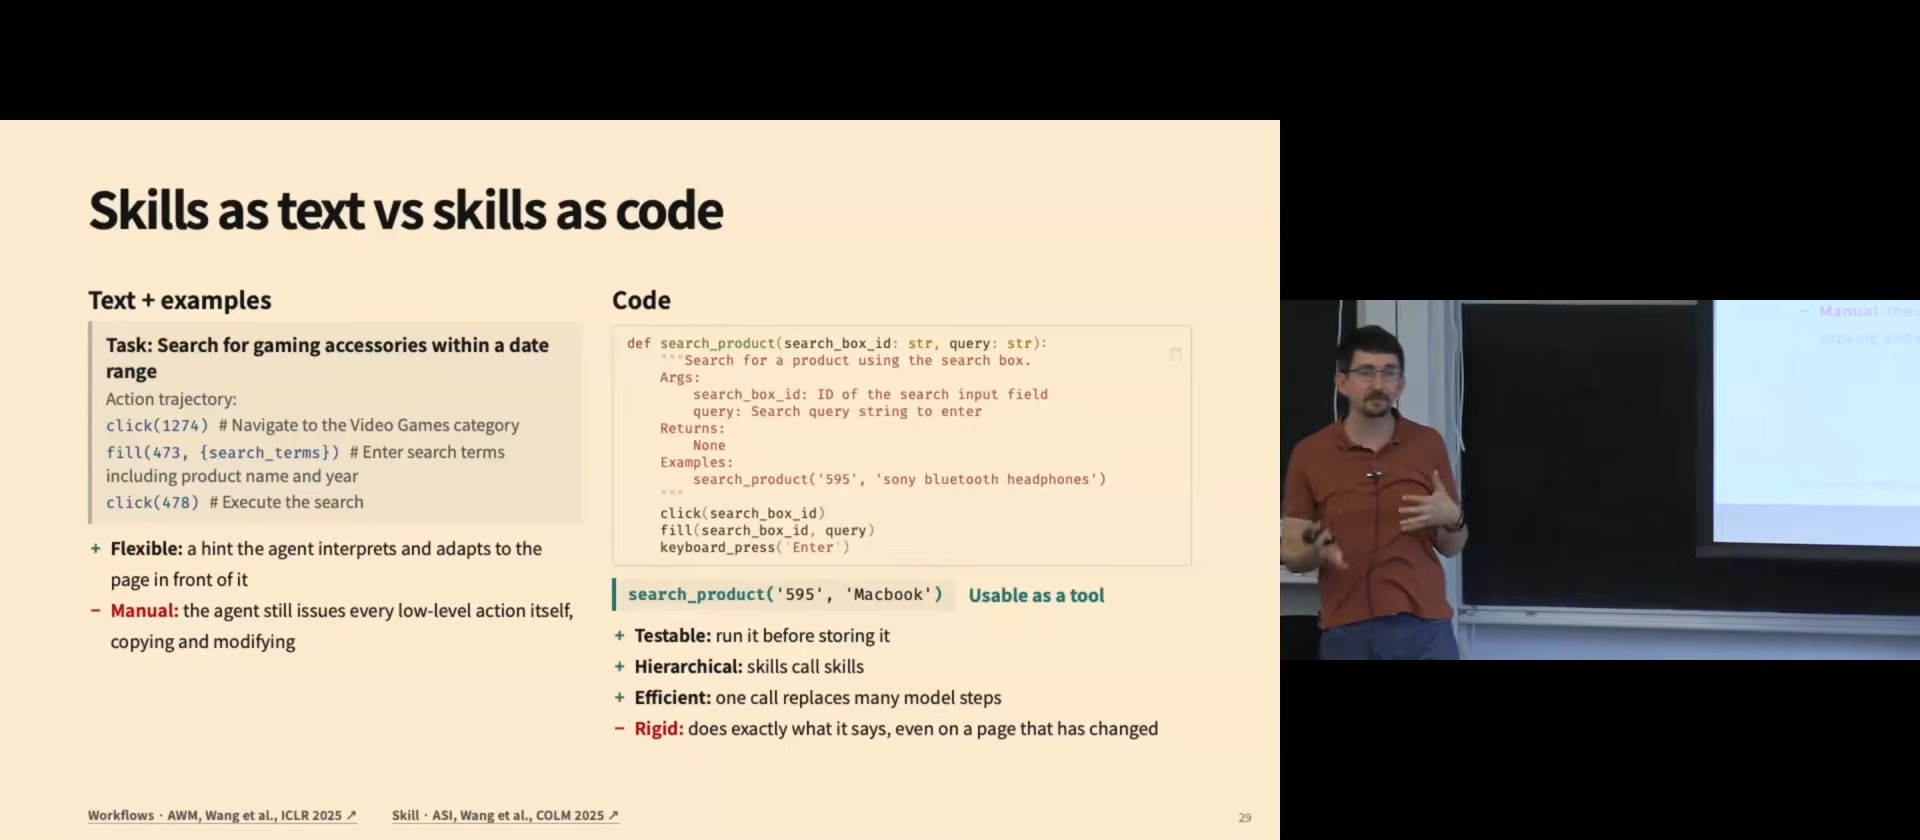
\includegraphics[width=\textwidth]{figures/fig_23_text_vs_code.jpg}
\caption{同一段搜索子过程的两种表示：文本加示例轨迹需要模型逐步重放动作，代码函数则把动作序列封装成一次可调用操作\vtag}

\end{figure}
\srcnote{00:57:15--00:57:30}

代码表示的好处不止省步数。函数可以嵌套，可以有自己的单元测试，因此可以脱离整条轨迹单独验证；函数还可以被重构。它的代价是刚性：函数内部的步骤被固定下来，环境一变化就没有回旋余地。本讲义把“技能可被组合”这件事写成下面的形式：若一件较复杂的技能由若干子技能组成，则它可以表示为

\[
\text{skill}_{\text{complex}} = g\bigl(\text{skill}_{1}, \text{skill}_{2}, \ldots, \text{skill}_{n}\bigr).
\]

\begin{itemize}
\item $\text{skill}_{i}$：已经学会的子技能，在代码表示中就是一个可调用的函数；
\item $g$：把子技能串起来的组合方式，在代码中通常是一段更外层的函数体；
\item $n$：参与组合的子技能数量。
\end{itemize}

组合能力让技能库像程序库一样增长：简单的函数先被学会，复杂的行为再通过调用它们实现。

\subsection{从轨迹归纳代码技能}

Agent Skill Induction 沿用 AWM 的整体框架，区别在于归纳的产物是代码。语言模型既善于写代码也善于读工具调用轨迹，于是它被要求生成抽象出轨迹行为的函数，并附上文档字符串；同时它还要把原来的轨迹改写成使用这些函数的版本。图~图 24 展示了归纳出的 search\_reviews 函数以及改写后的轨迹。

\begin{figure}[H]
\centering
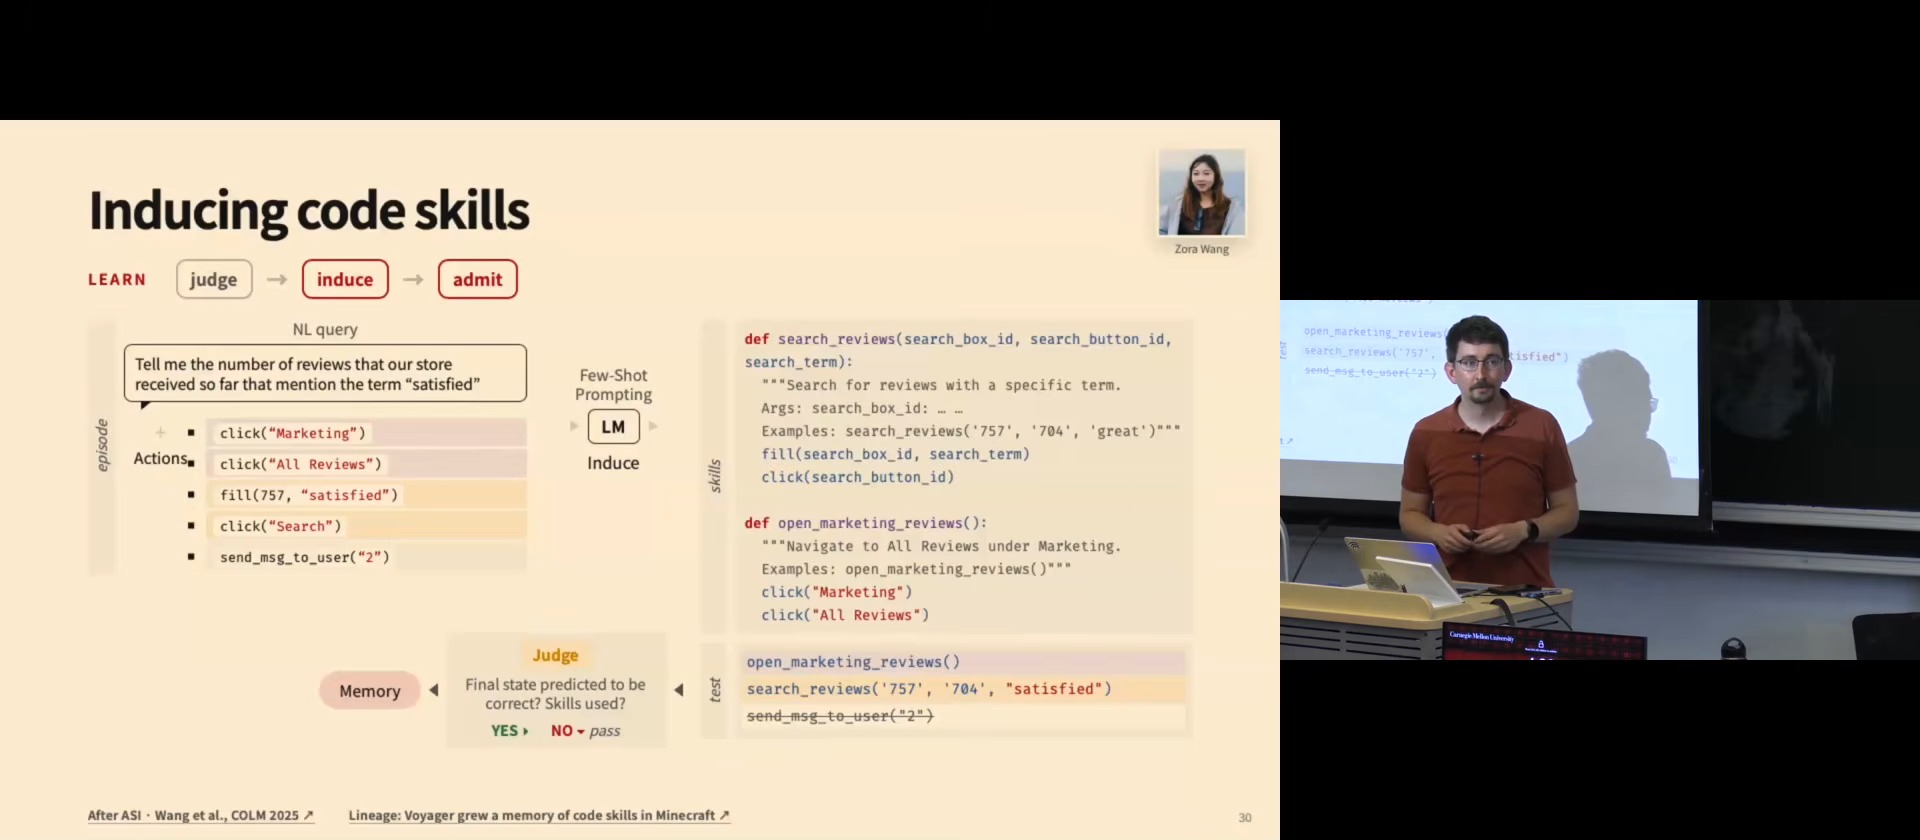
\includegraphics[width=\textwidth]{figures/fig_24_asi_code_skills.jpg}
\caption{Agent Skill Induction：从工具调用轨迹归纳出带文档字符串的代码函数，并把原轨迹改写成调用这些函数的版本\vtag}

\end{figure}
\srcnote{00:59:15--00:59:30}

代码表示带来一个文本表示没有的验证手段：函数可以被真正执行。系统不需要只对原始轨迹做裁判，而是可以执行抽象后的代码，再对执行结果做裁判。视频认为这是更强的正确性信号，因为一个能跑通并产生正确结果的函数，比一段“看起来对”的描述更可信。通过验证的函数作为工具进入记忆，模型在后续任务里直接调用它们。

\begin{lstlisting}[caption={从轨迹归纳出的代码技能（据视频第 26、27 页）},language=Python]
def search_reviews(search_box_id, search_button_id, search_term):
    """Search for reviews with a specific term.

    Args:
        search_box_id: id of the reviews search input
        search_button_id: id of the search submit button
        search_term: term to look for
    Examples:
        search_reviews("757", "704", "great")
    """
    ...
\end{lstlisting}

\subsection{代码技能的测试与修订}

代码技能可以被单独测试，因此技能本身的质量有了独立的检查入口。SkillWeaver 把收录过程写成一段循环：先为任务提出一组候选技能，再用它们实际执行任务得到一条轨迹，然后由奖励模型判断是否成功；成功就把技能加入记忆，失败就修订候选技能。图~图 25 给出了这段伪代码，以及一个真实的修订例子。

\begin{lstlisting}[caption={SkillWeaver 的技能收录循环（据视频第 28 页）},language=Python]
candidates = propose_skill(task)
episode = practice(candidates, task)
if reward_model(episode.actions, episode.screenshots, task):
    memory.add(candidate)
else:
    candidate = revise(candidate, task)
\end{lstlisting}

\begin{figure}[H]
\centering
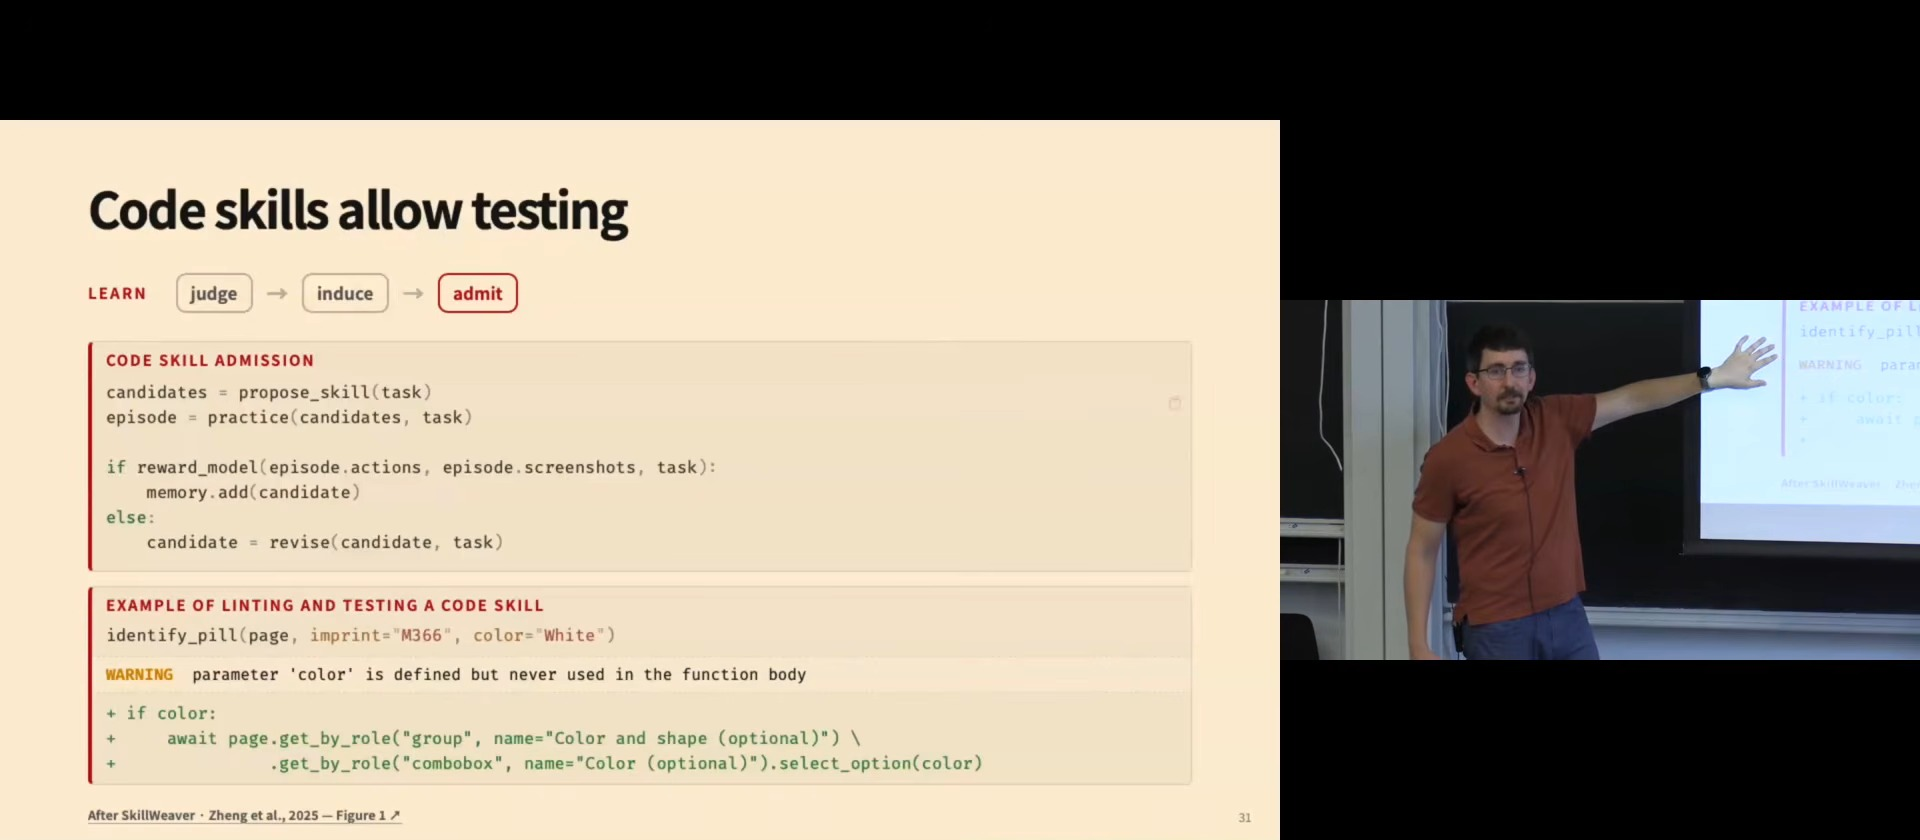
\includegraphics[width=\textwidth]{figures/fig_25_skillweaver_testing.jpg}
\caption{代码技能允许单独测试：SkillWeaver 的收录循环，以及代码检查器发现 identify\_pill 函数声明了 color 参数却从未使用后给出的告警\vtag}

\end{figure}
\srcnote{01:00:30--01:00:45}

例子中，智能体为药品网站写了一个 identify\_pill 函数，签名里包含 imprint 与 color 等参数，但函数体从未使用 color。代码检查器直接给出“参数 color 已定义但从未在函数体中使用”的告警，这类反馈可以像上一节的反思一样被条件化，用来生成修订版函数。也就是说，代码技能既受益于文本技能那套裁判反馈，又额外获得了静态检查这一层信号。

\subsection{任务压缩与效率收益}

代码技能最直观的收益是压缩步数。视频给出的任务是把账单地址改成 231 Willow Way, Suite 100, Chicago, IL, 60601，再把收货地址改成 987 Sycamore Circle, Philadelphia, PA, 19102。没有记忆时，智能体要逐步导航、逐个表单填写、逐次保存；有了归纳出的 navigate\_to\_address\_settings 与 update\_address\_details 两个函数后，同一件事可以压成少数几步。图~图 26 对照了两种执行方式。

\begin{figure}[H]
\centering
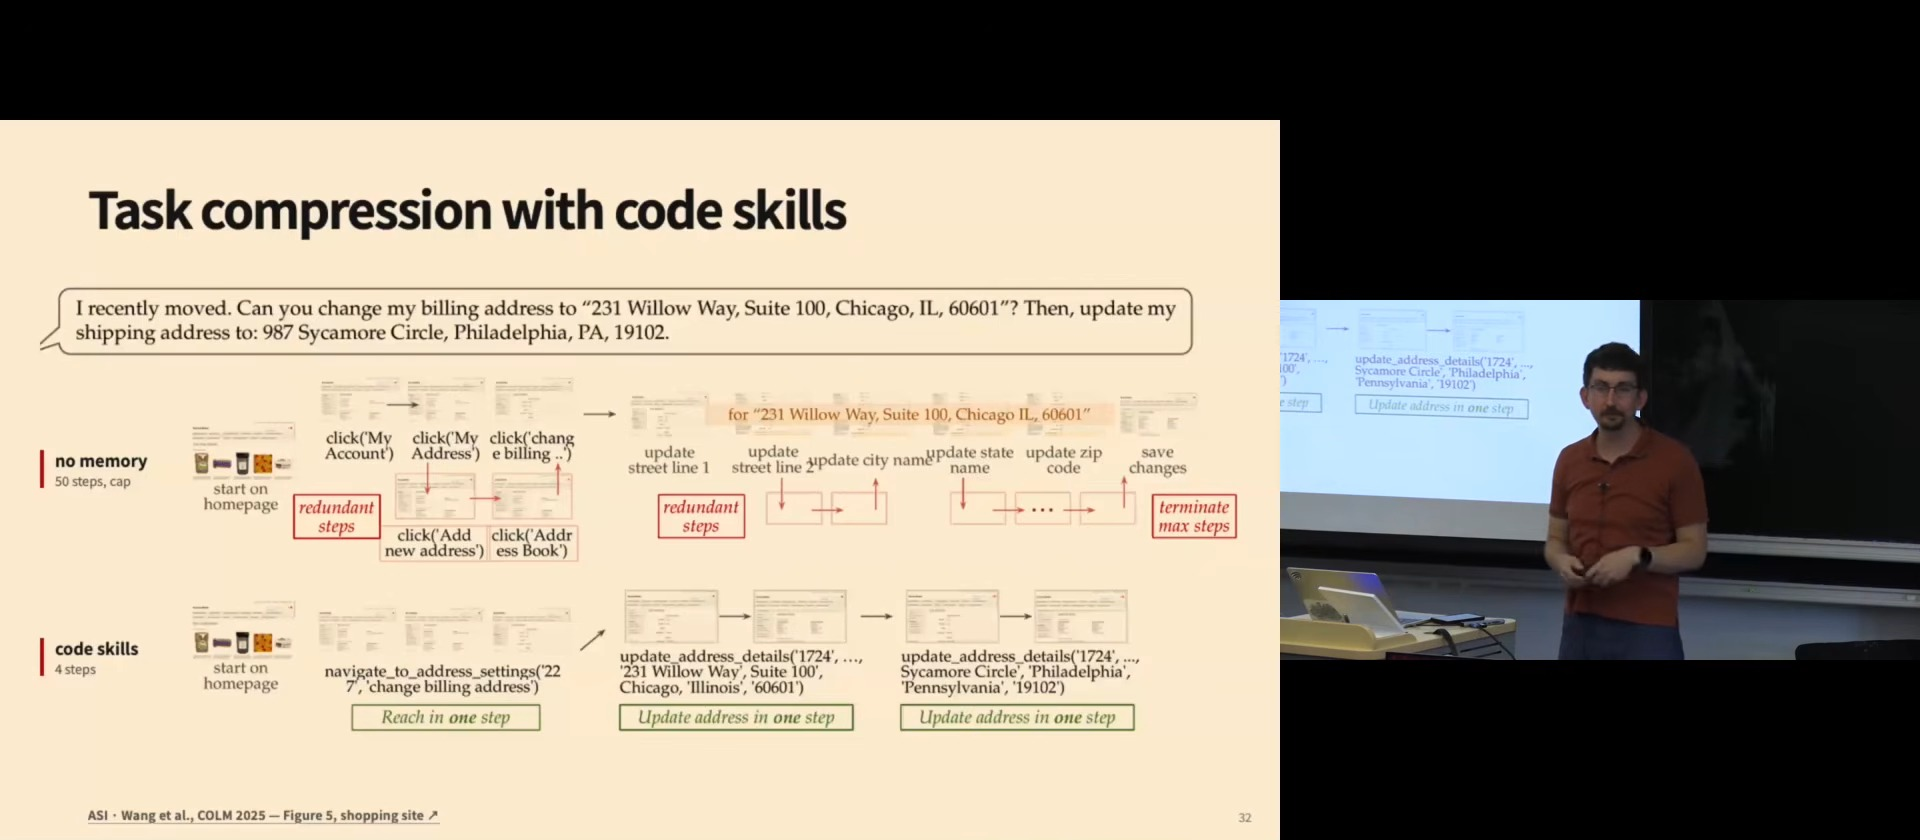
\includegraphics[width=\textwidth]{figures/fig_26_task_compression.jpg}
\caption{代码技能压缩任务步数：两次地址更新从逐步点击表单变成调用 update\_address\_details 等函数完成\vtag}

\end{figure}
\srcnote{01:02:15--01:02:30}

效率收益在这个场景里格外重要。视频解释，网页智能体的两大开销是反复观察页面（截图占据大量 token）和为每个动作生成思维链；代码技能把多次“观察、思考、动作”的循环折叠成一次函数调用，因此同时减少了 token 消耗和往返次数。图~图 27 给出了受控比较的结果：在具有重复结构的网页任务上，无记忆、文本技能与代码技能三者的检查点达成率分别是 41.3、59.5 与 80.2，平均每任务步数分别是 24.5、20.6 与 15.0。

\begin{figure}[H]
\centering
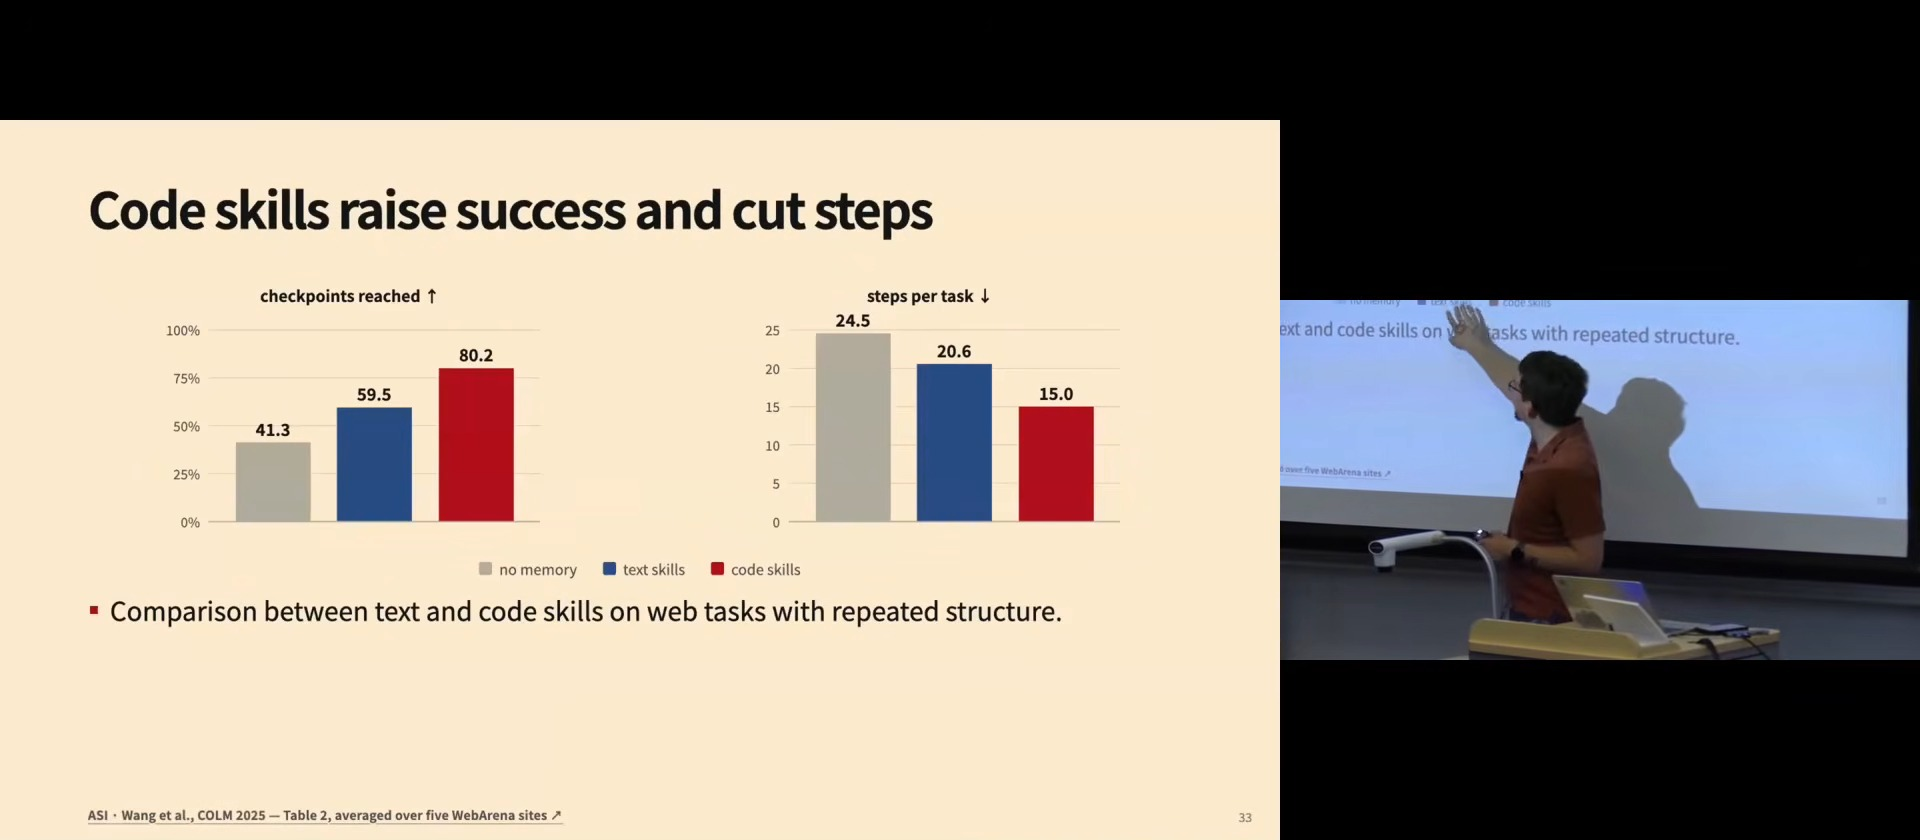
\includegraphics[width=\textwidth]{figures/fig_27_code_text_results.jpg}
\caption{文本技能与代码技能的对照结果：检查点达成率从 41.3 提升到 59.5 再到 80.2，每任务步数从 24.5 降到 20.6 再到 15.0\vtag}

\end{figure}
\srcnote{01:02:45--01:03:00}

\begin{knowledgebox}{为什么网页任务里步数如此关键}
每一次与环境交互都要重新观察页面（截图是昂贵的 token），并为下一个动作生成思维链。代码技能把多次“观察、思考、动作”的循环折叠成一次函数调用，于是同时减少了观察与推理两方面的开销。这就是为什么在重复结构较强的网页任务上，效率提升与成功率提升会同时出现。
\end{knowledgebox}

\begin{importantbox}{文本与代码不是二选一}
两种表示各有清晰的适用面。文本技能给出灵活指导，适合环境会变化、需要模型临场判断的场合；代码技能给出可执行的固定动作，适合流程稳定、重复度高、追求效率的场合。当前标准允许一个技能包同时包含文本正文与脚本，如何把两者组合起来，视频把它列为仍有待研究的问题。
\end{importantbox}

\subsection{本章小结}

文本工作流把轨迹抽象成模板，代码技能把模板进一步固化成可调用、可测试的函数。代码在效率和可验证性上占优，代价是刚性。接下来要回答的正是这种刚性的后果：当环境变化时，技能还能不能迁移。

\section{技能的泛化、抽象与记忆整理}

\subsection{当技能遇上不同的网站}

代码技能的刚性会在跨站点时暴露。视频展示了一个失败案例：技能在某个站点上归纳出来后，被应用到真实的 Target 购物网站；技能假设排序控件是一个下拉菜单，而 Target 用的是单选按钮，于是技能直接失效。这里的教训不是“不要用代码”，而是技能必须能够根据环境反馈被修改。图~图 28 画出了这个失败场景，并给出一个量化读数：只有约四分之一的情形能正确复用已学技能。

\begin{figure}[H]
\centering
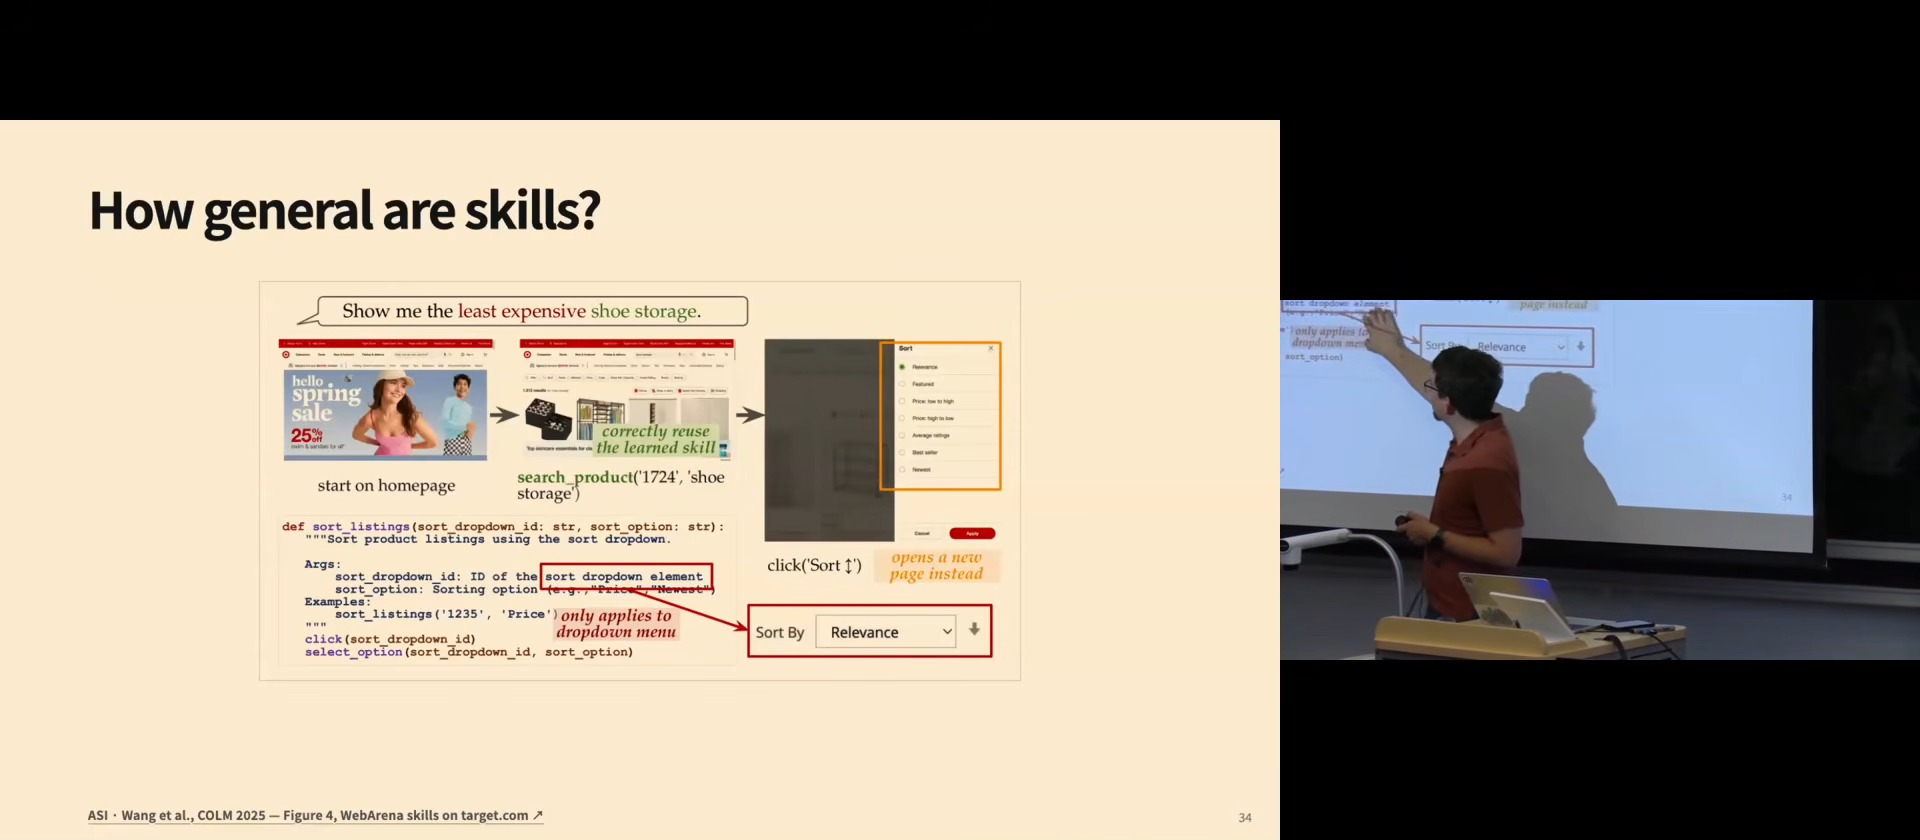
\includegraphics[width=\textwidth]{figures/fig_28_generalization_failure.jpg}
\caption{技能跨站点泛化失败：在别的站点归纳出的技能假设排序控件是下拉菜单，遇到 Target 的单选按钮即失效\vtag}

\end{figure}
\srcnote{01:03:45--01:04:00}

\subsection{用抽象类分离接口与实现}

软件工程对“同一接口、多种实现”早有成熟做法，视频介绍的 PolySkill 把它搬到技能上。第一次与某个新网站交互时，模型先写一个抽象类，定义 search\_product、add\_to\_cart、checkout 这类方法的接口，方法体留空或只写占位；然后再写这个网站的具体实现。当智能体换到另一个网站时，已有的具体实现不再适用，模型据此写出同一抽象类的另一个实例。图~图 29 给出了抽象类与 Amazon 实现并置的结构。

\begin{figure}[H]
\centering
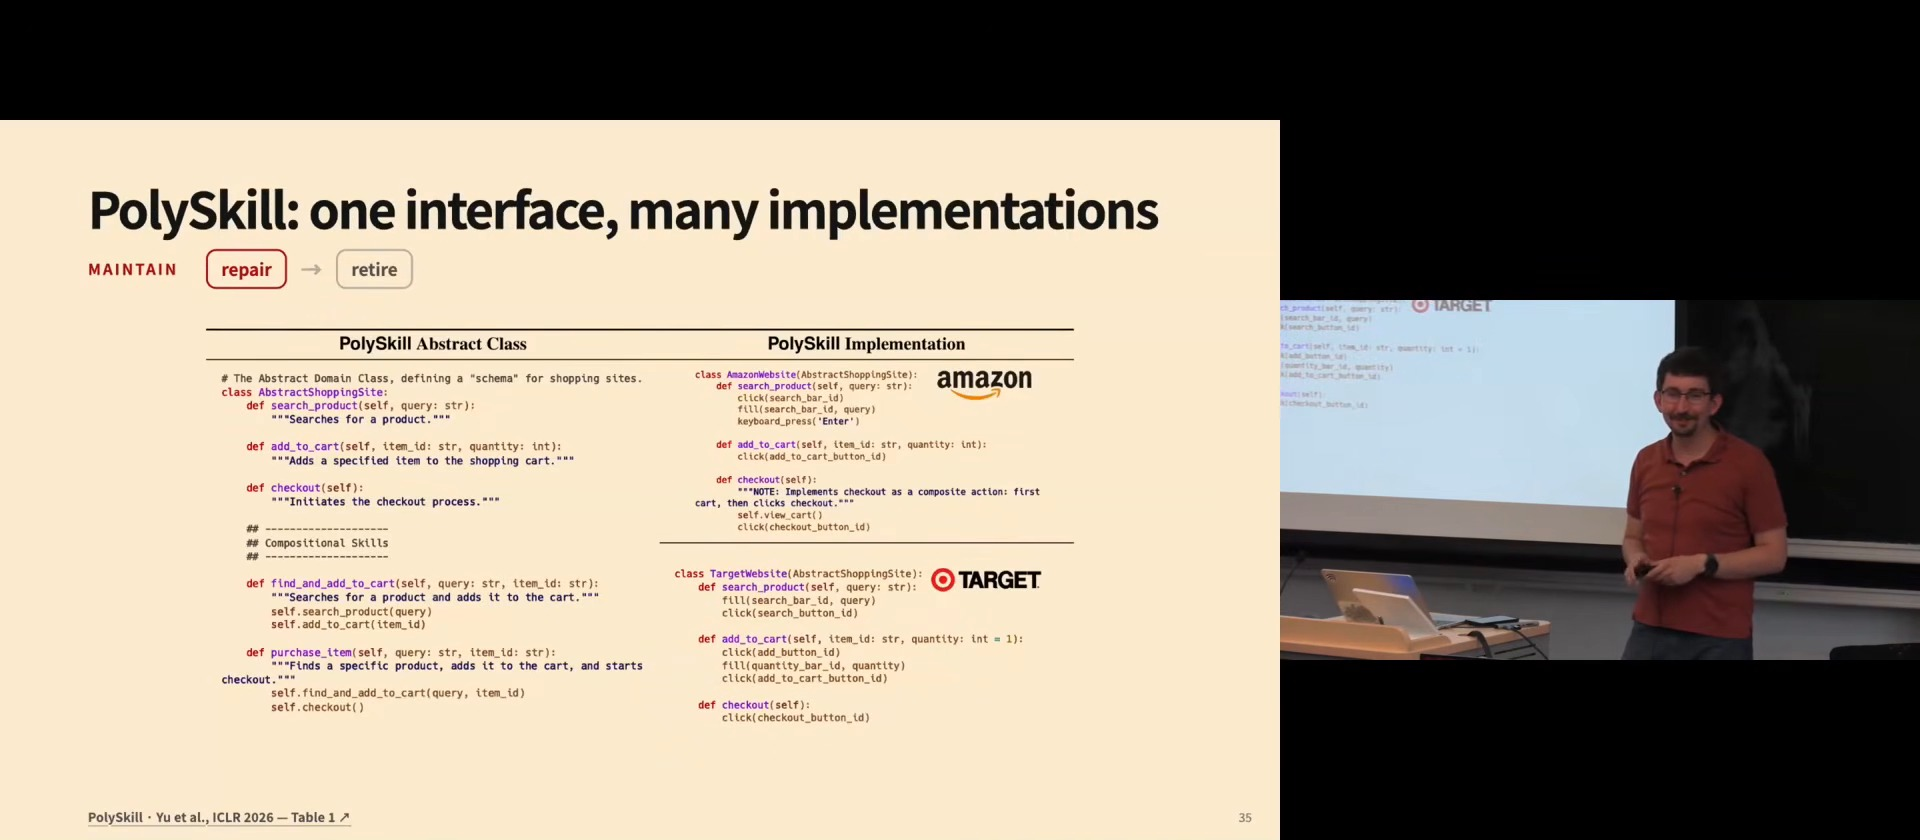
\includegraphics[width=0.88\textwidth]{figures/fig_29_polyskill_abstraction.jpg}
\caption{PolySkill：抽象类定义购物站点的接口契约，各站点提供具体实现，换站点时实例化新的实现\vtag}

\end{figure}
\srcnote{01:04:15--01:04:30}

这个结构还顺带解决了规模问题：技能库里可以保留大量站点专属的实现，但任一时刻只有与当前站点相关的那个子集被激活，因此上下文不必容纳全部实现。视频把它总结为一条软件工程最佳实践向智能体的迁移。

\subsection{三种表示法的取舍}

到了这里，三种表示法的差异可以放在一张表里。视频用一页幻灯片给出了对照，图~图 30 是原图，表~表 1 按同样的内容整理。

\begin{figure}[H]
\centering
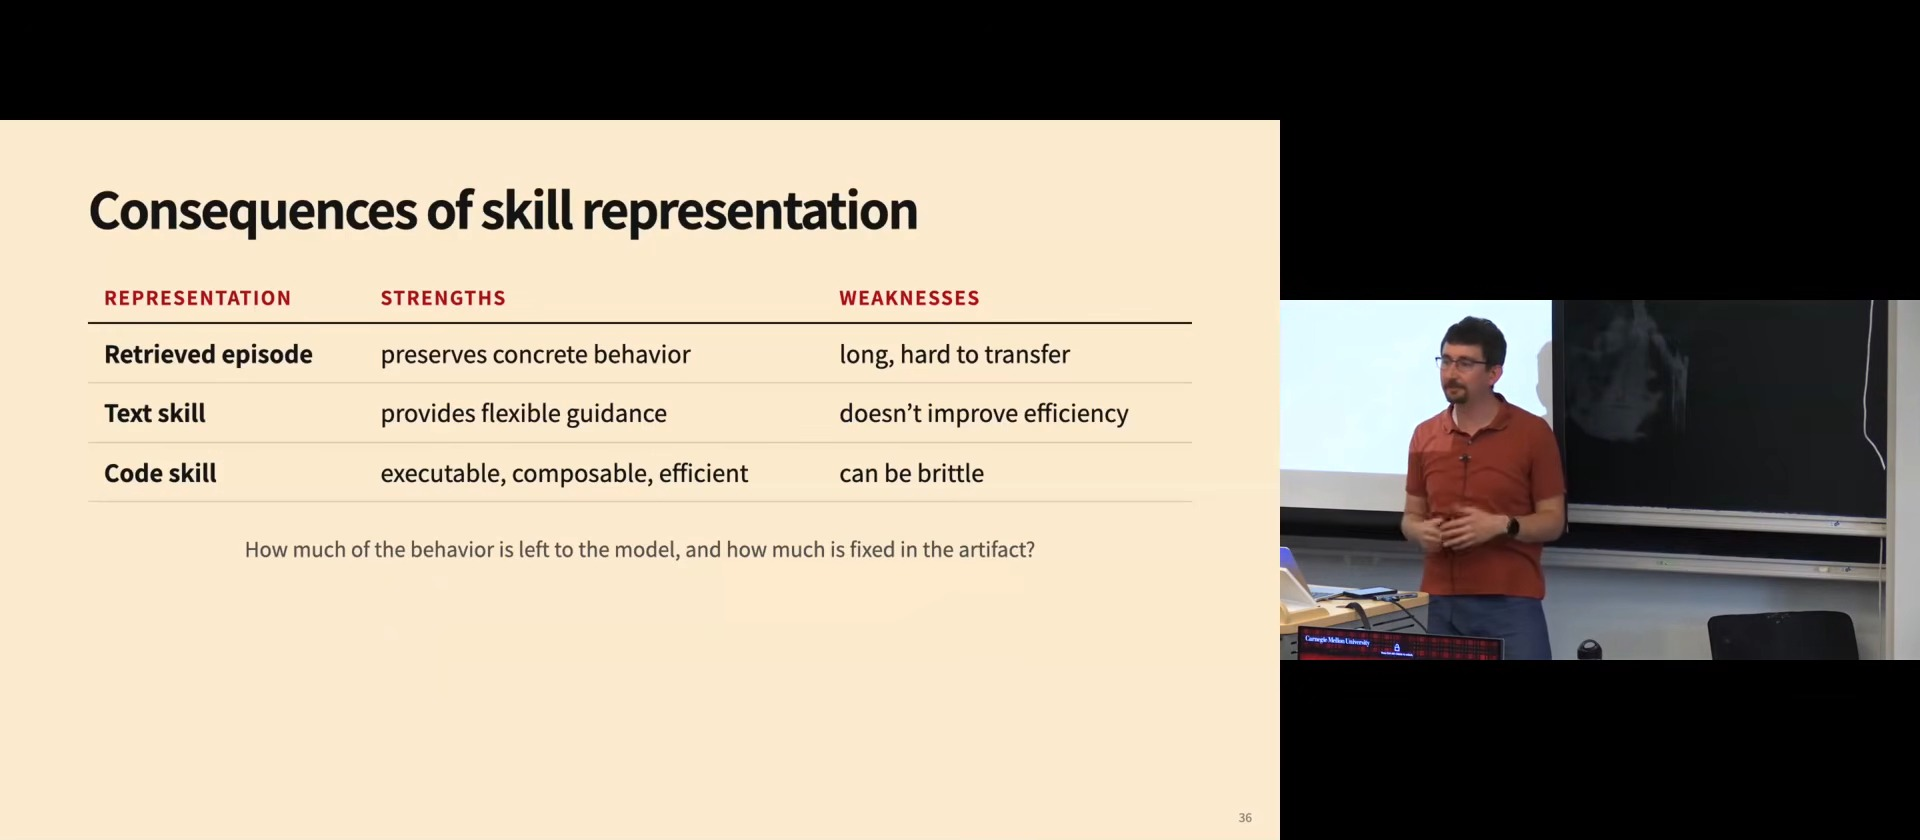
\includegraphics[width=\textwidth]{figures/fig_30_representation_tradeoffs.jpg}
\caption{检索轨迹、文本技能与代码技能的强项与弱点对照，末行追问行为有多少交给模型、多少固定在工件里\vtag}

\end{figure}
\srcnote{01:05:45--01:06:00}

\begin{table}[H]
\centering
\caption{三种技能表示法的强项与弱点（据视频第 36 页整理）}

\begin{tabular}{p{2.6cm}p{5.4cm}p{5.4cm}}
\toprule
表示法 & 强项 & 弱点 \\
\midrule
检索轨迹 & 保留具体行为 & 很长，难以迁移 \\
文本技能 & 提供灵活指导 & 不提升效率 \\
代码技能 & 可执行、可组合、效率高 & 可能很脆弱 \\
\bottomrule
\end{tabular}
\end{table}表下方的追问是这一节的核心：行为有多少留给模型，多少固定在工件里。固定得越多，效率和可验证性越好，但适应性越差；留给模型的越多，适应性越强，但每一步都要重新付出推理与观察的代价。技能设计本质上是在这条轴上做选择。

\subsection{记忆整理：让技能库不无限膨胀}

技能库会随时间增长，而检索到越多不相关的技能，模型越容易被干扰。视频介绍了一种按使用频次整理的思路：记录每个函数被用到的次数，若使用次数低于某个与样本量相关的阈值就删掉它。TroVE 采用的做法是删除使用次数少于 $\log_{10}(n)$ 的函数，其中 $n$ 是样本数。图~图 31 展示了在 MATH、Algebra、HiTab 与 GQA 等数据集上，开启遗忘后函数库规模分别压缩到原来的 74、83 与 90（百分比），同时性能没有明显损失。

\begin{figure}[H]
\centering
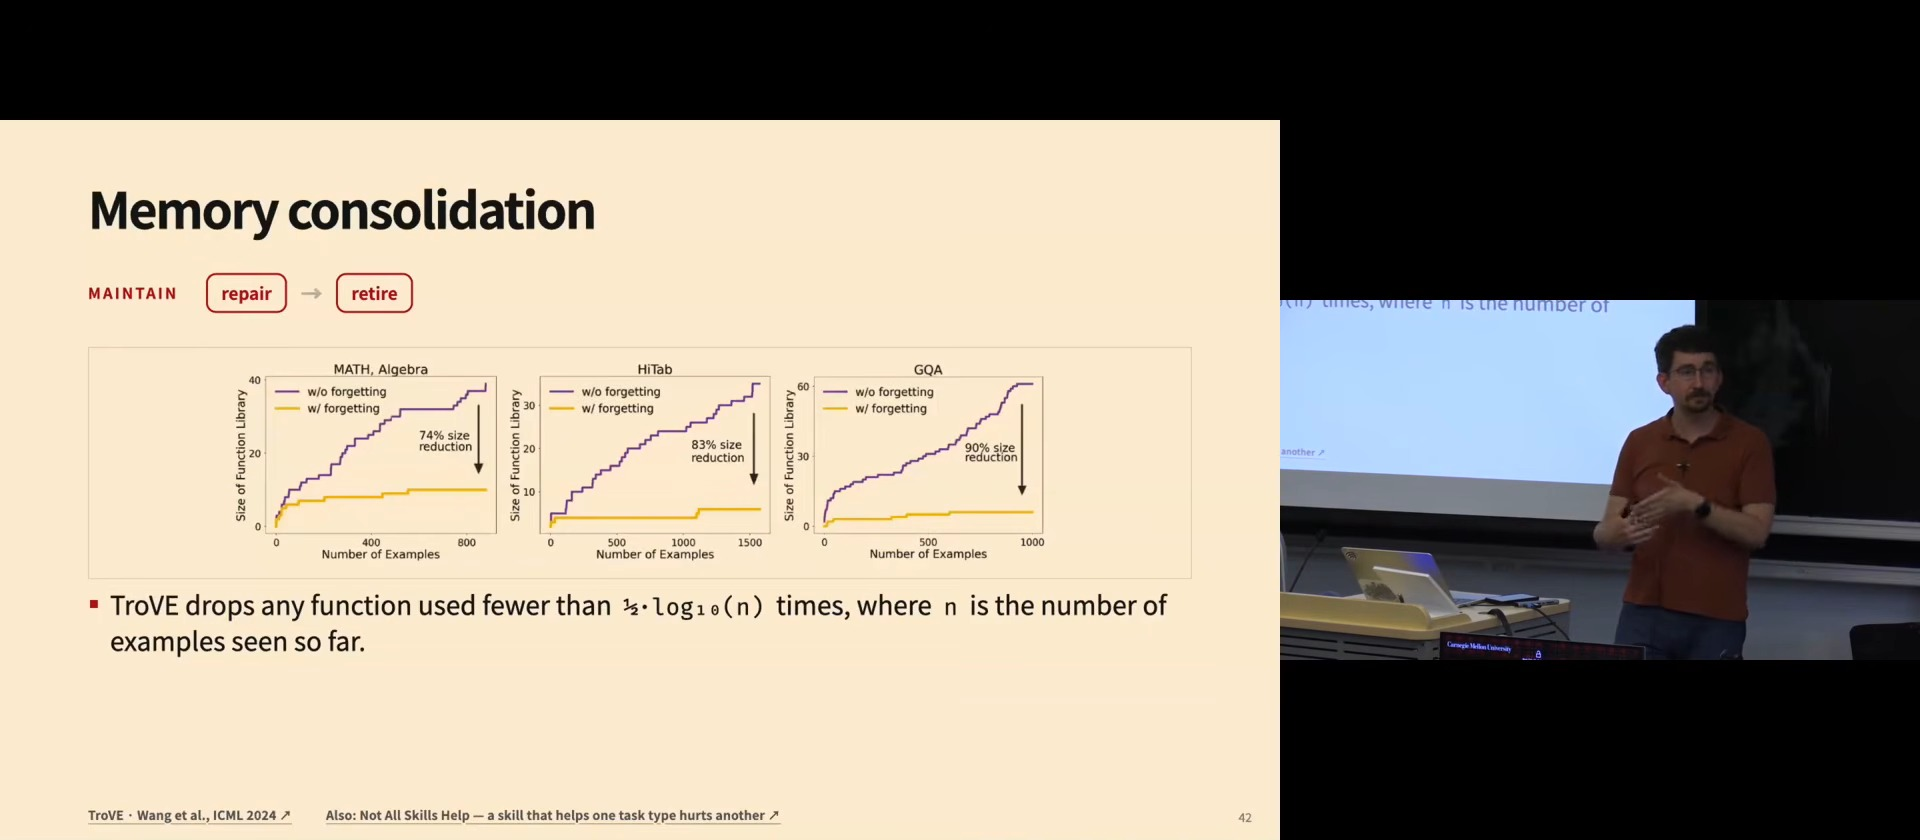
\includegraphics[width=\textwidth]{figures/fig_35_memory_consolidation.jpg}
\caption{记忆整理：按使用频次淘汰函数，三组实验把函数库规模分别压缩到 74\%、
83\%
与 90\%，性能基本保持\vtag}
\end{figure}
\srcnote{01:12:00--01:12:15}

\begin{knowledgebox}{整理是维护的一部分}
淘汰低频函数既是效率手段，也是性能手段。效率上，检索池更小、上下文更短；性能上，模型被无关技能干扰的机会更少。这与前面“技能太多反而变差”的观察是一致的，说明记忆容量并不是越大越好。
\end{knowledgebox}

\subsection{本章小结}

技能跨站点失效说明代码表示需要抽象层，PolySkill 用抽象类与具体实现分离了接口和行为。三种表示法各有代价，整理机制则控制技能库的规模。到这里，技能的产生、使用和维护已经完整。最后一节回过头来看两个更基础的问题：记忆内容的质量，以及能否直接训练出会归纳技能的模型。

\section{记忆质量、规模与训练}

\subsection{从失败中学习}

前面的归纳都建立在成功轨迹上，但失败同样有信息量。视频举了一个具体的失败：任务要求给出 Sony 蓝牙耳机的完整名称，并给出可选型号的价格区间；该网站的检索默认按“或者”匹配，于是一个笼统的查询返回了 5,578 条结果。智能体被迫在大量结果中翻页，逐渐丢失了任务目标，最终失败。反思这条失败轨迹后得到的不是一条新轨迹，而是一段文本策略：查询过于笼统，答案被淹没在成千上万条弱相关的结果里，应当在浏览前收紧查询；同时可以调整每页显示条数，让模型一次看到更多条目。图~图 32 同时给出了原始任务、失败轨迹与归纳出的两条策略。

\begin{figure}[H]
\centering
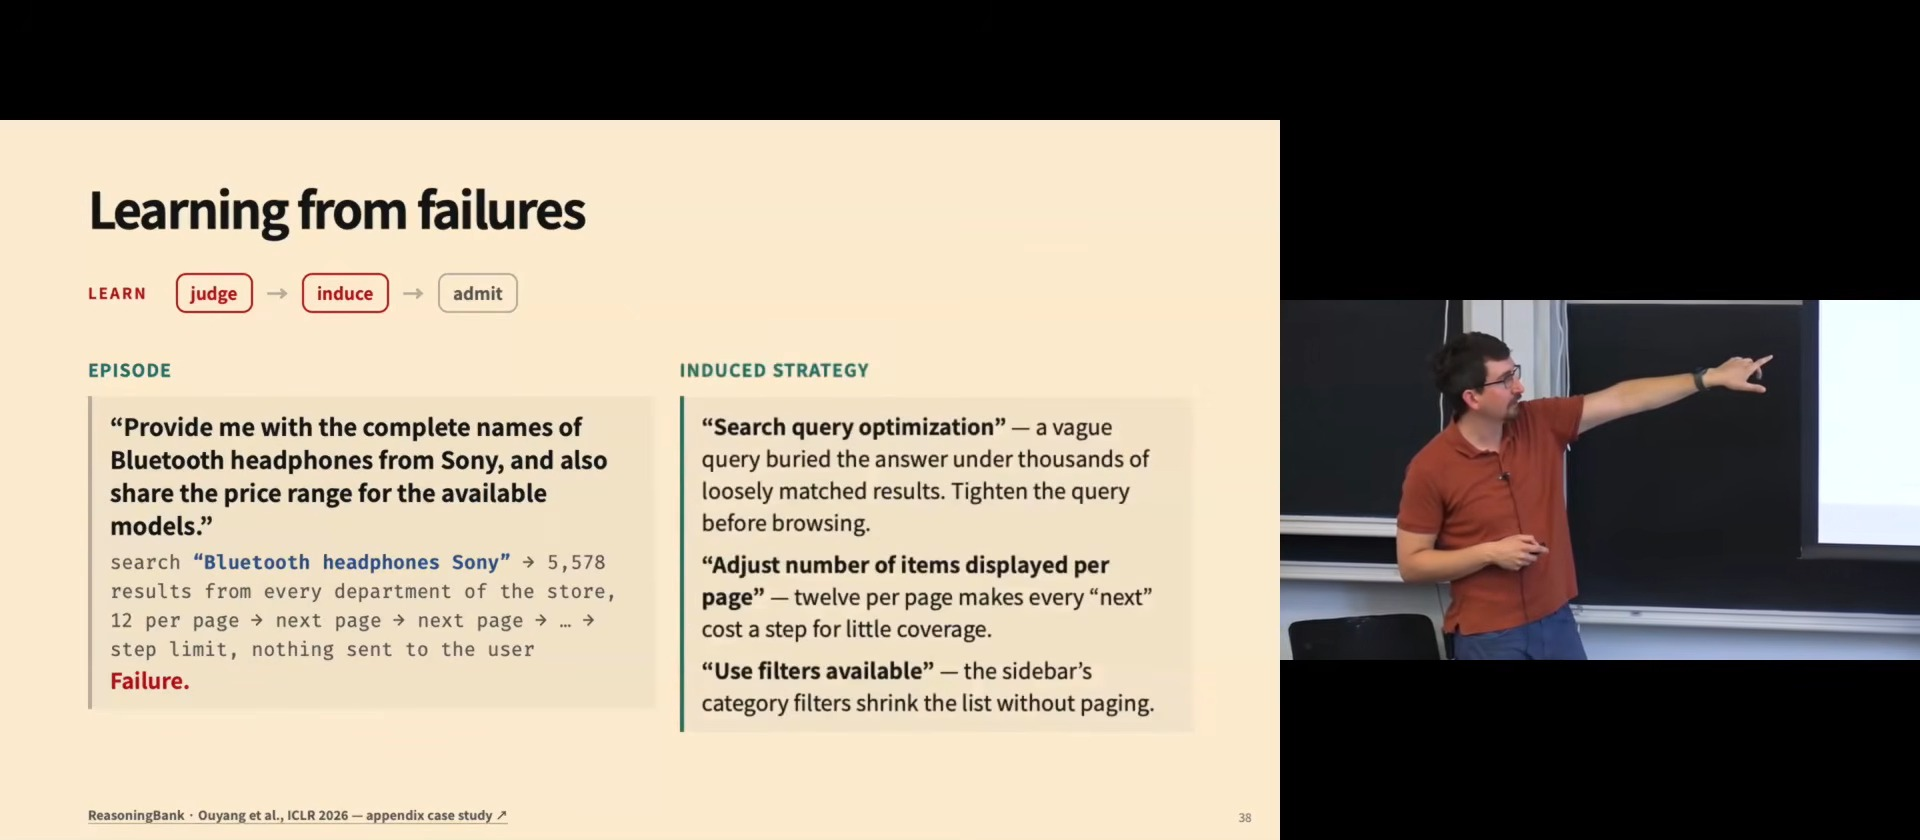
\includegraphics[width=\textwidth]{figures/fig_31_learning_from_failures.jpg}
\caption{从失败中学习：一次返回 5,578 条结果的失败检索，被归纳成“收紧查询”与“调整每页显示条数”两条文本策略\vtag}

\end{figure}
\srcnote{01:07:00--01:07:15}

把失败写成文本策略，而不是把失败轨迹原样存起来，是这里的关键设计。失败的轨迹往往很长，而且包含大量与教训无关的细节；一段一般化的描述反而更容易在新任务中被正确使用。

\subsection{失败案例对不同记忆类型的影响}

视频用一组受控实验检验了“加入失败案例”的后果，结果并不一致。图~图 33 的柱状图对比了 Synapse（整条轨迹）、AWM（工作流）与 ReasoningBank（文本策略）三类记忆，在只用成功案例与同时使用失败案例两种条件下的成功率。图中的读数包括 49.7、46.5、44.4、42.2、41.7 与 40.6，并标注无记忆基线为 39.0。从柱状图的整体形状看，以整条轨迹或工作流为记忆的条件在加入失败案例后下降，而以文本策略为记忆的条件上升。

\begin{figure}[H]
\centering
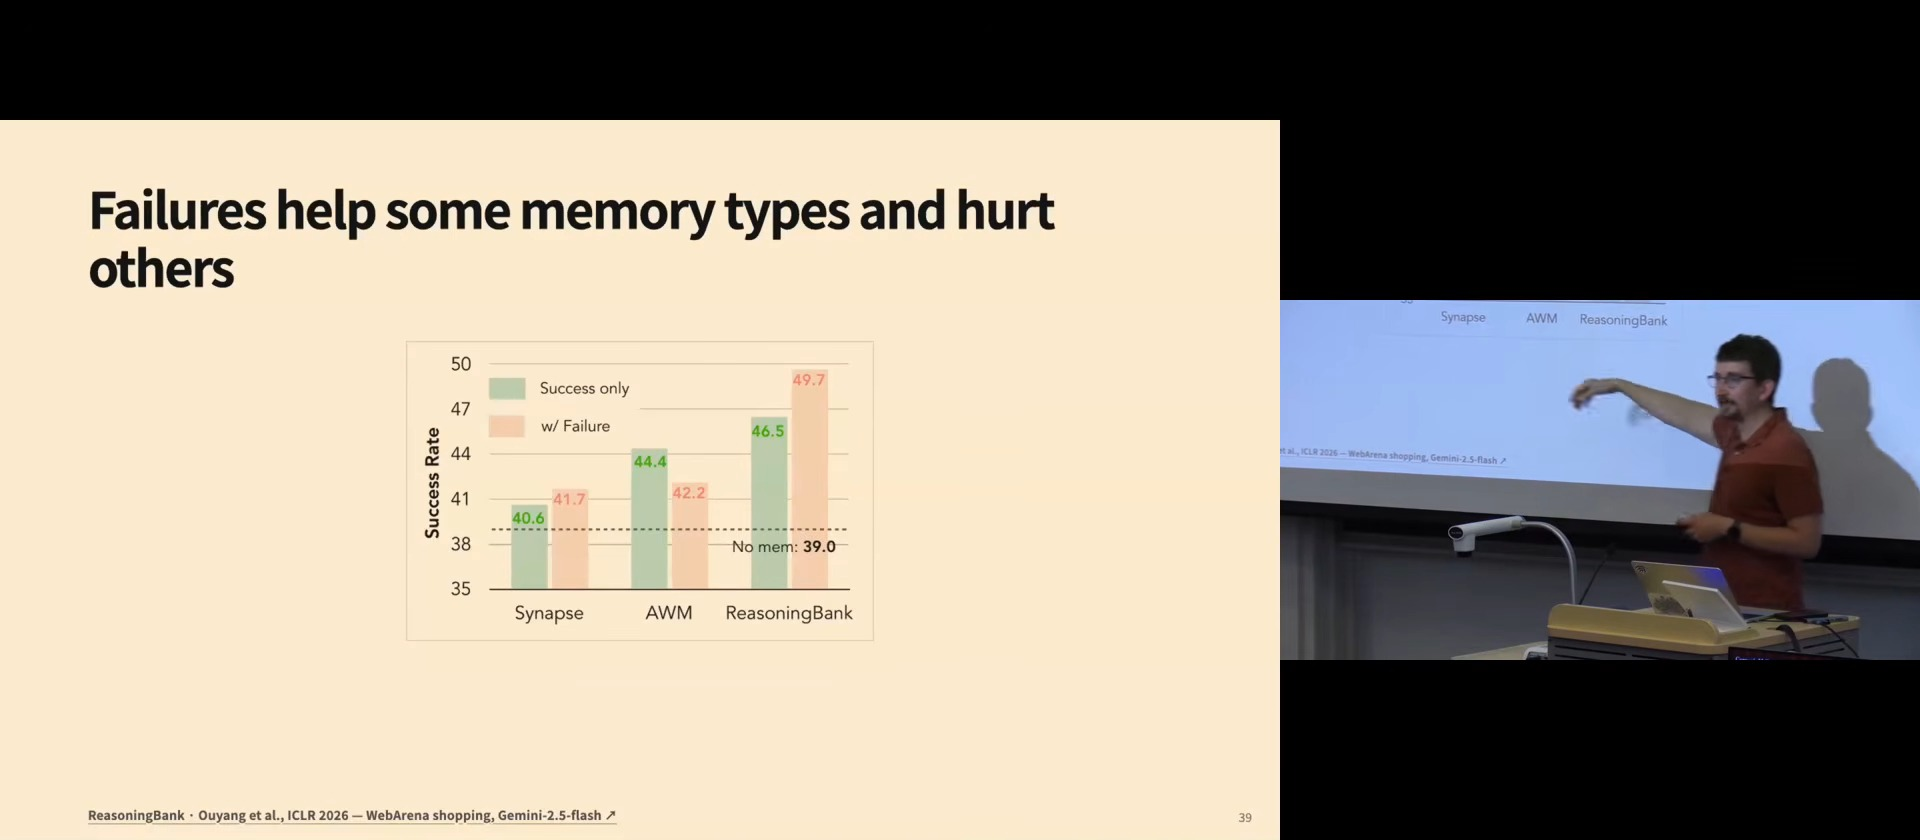
\includegraphics[width=\textwidth]{figures/fig_32_failures_memory_types.jpg}
\caption{失败案例对不同记忆类型的影响：整条轨迹与工作流在加入失败案例后下降，文本策略类记忆上升；无记忆基线为 39.0\vtag}

\end{figure}
\srcnote{01:08:00--01:08:15}

这个结果与直觉一致：一段具体的失败轨迹里，真正要传达的教训被埋在大量细节中，模型可能照抄了错误的做法；而一段“应当收紧查询”的文本策略本身就剥离了细节，只保留可迁移的判断。视频由此把“存什么形态的记忆”列为一个独立的设计维度，与“存不存”同等重要。

\subsection{裁判准确率有多重要}

如果记忆的收录依赖裁判，那么裁判的错误会直接影响记忆质量。视频介绍了一组消融实验：先用真实标签模拟理想裁判，再按固定概率翻转标签，模拟从完美裁判到随机裁判的各种准确率。图~图 34 画出了成功率随模拟裁判准确率变化的曲线，横轴从 100 到 50，纵轴读数包括 52.4、51.8、50.6、49.4、49.7、48.7、48.2、47.6 与 47。整体趋势是随裁判变差而下降，但下降相对平缓，在相当宽的准确率范围内仍然优于无记忆基线。

\begin{figure}[H]
\centering
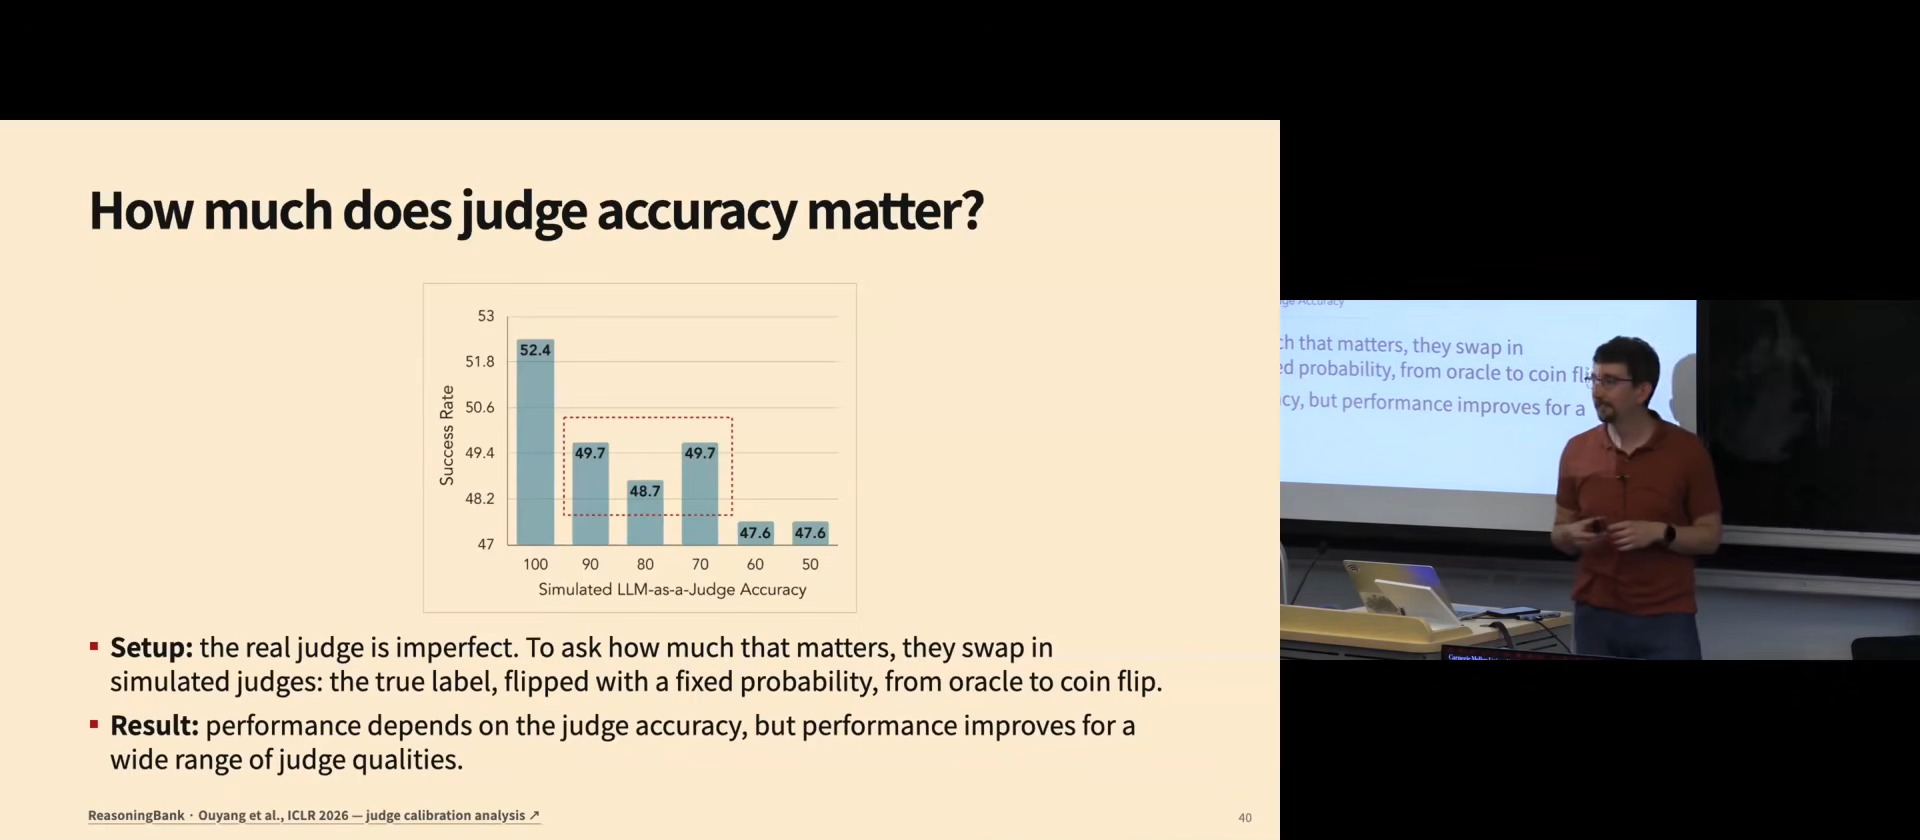
\includegraphics[width=\textwidth]{figures/fig_33_judge_accuracy.jpg}
\caption{裁判准确率消融：从理想裁判到随机裁判，成功率从 52.4 逐步降到 47 附近，但在较宽的准确率区间内仍然有用\vtag}

\end{figure}
\srcnote{01:09:15--01:09:30}

\begin{importantbox}{不完美的裁判不等于不可用}
消融的结论不是“裁判必须完美”，而是性能随裁判质量平滑变化，并且存在一个较宽的可用区间。真正的风险出现在裁判严重偏向某一类错误时：错误的正例会污染记忆，并在后续任务里被反复复用。这也是为什么维护阶段必须保留删除和修订的入口。
\end{importantbox}

\subsection{过度检索的代价}

记忆越多，检索时越容易召回不相关的条目，这会直接伤害性能。图~图 35 把成功率画成召回经验数量的函数：随着召回的条目增多，成功率从 45.5 依次降到 44.4、41 与 39。视频把这个现象归因于两个可能的原因：一是记忆里确实没有与当前任务相似的经验，硬塞进去的内容必然不相关，这是方法在此设定下的根本限制；二是模型本身不擅长在长上下文里排除干扰，这一条有可能通过训练改善。

\begin{figure}[H]
\centering
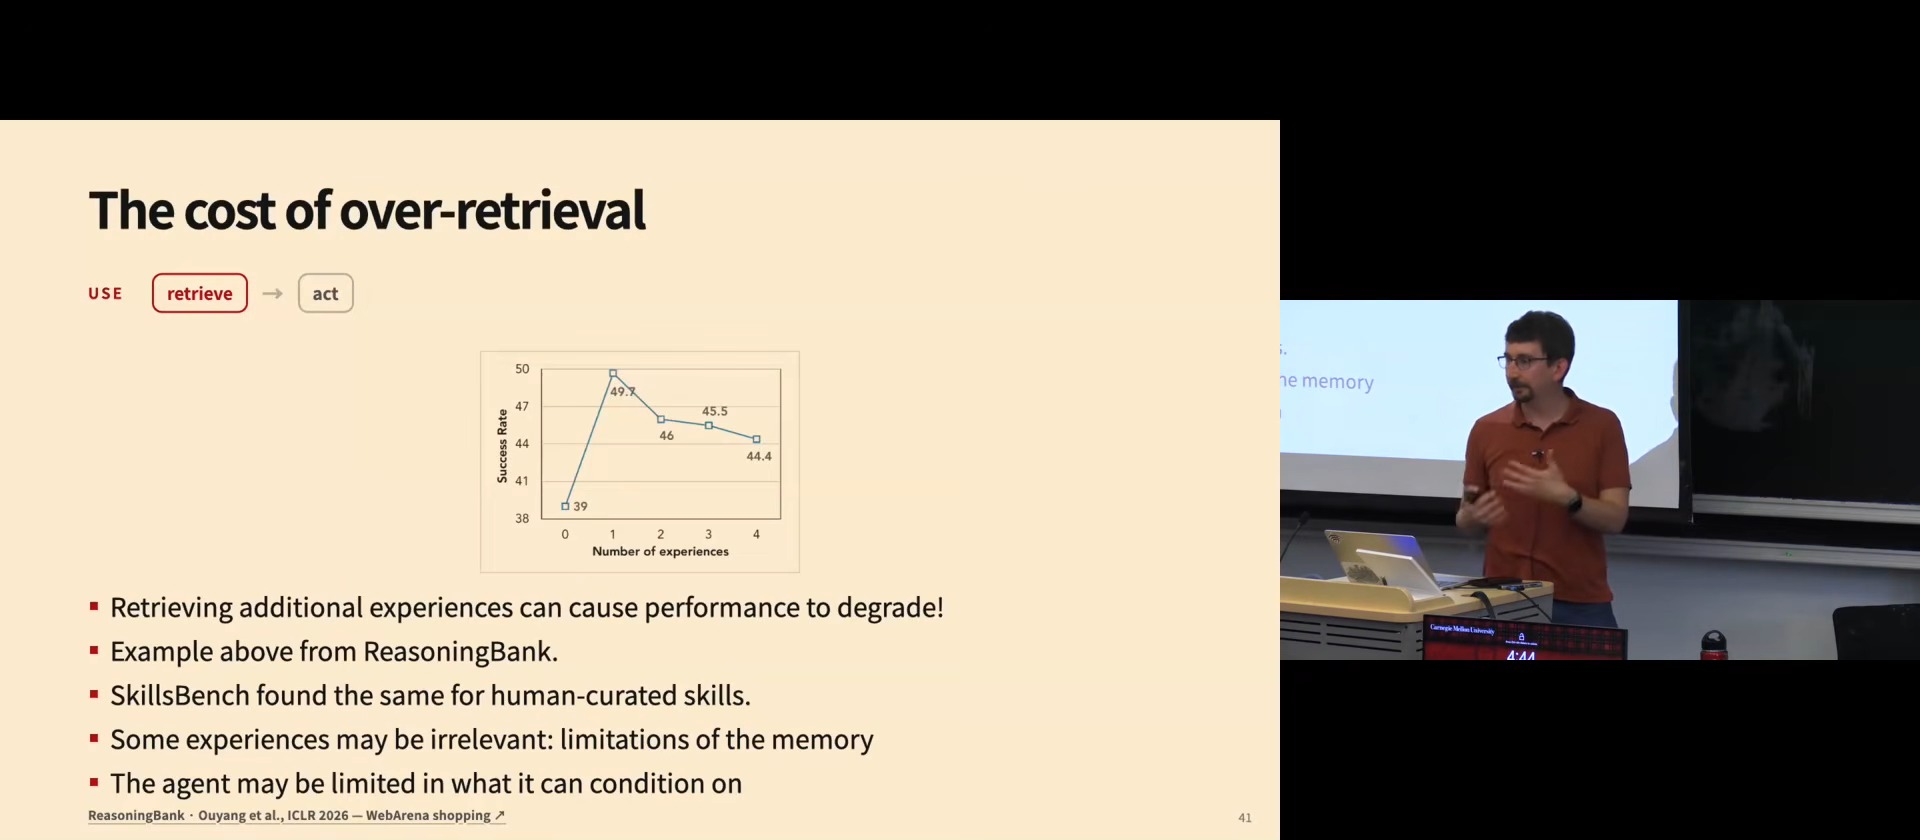
\includegraphics[width=\textwidth]{figures/fig_34_over_retrieval.jpg}
\caption{过度检索的代价：召回更多经验时成功率从 45.5 降到 44.4、41 直至 39；SkillsBench 在人工技能上也观察到同样趋势\vtag}

\end{figure}
\srcnote{01:10:30--01:10:45}

这两条解释指向不同的应对方式。如果问题出在记忆里没有相关内容，那么应当扩大记忆规模或改进归纳；如果问题出在模型被长上下文干扰，那么应当改进检索精度、缩短上下文，或者直接训练模型更好地忽略无关内容。

\subsection{训练技能归纳器}

至此所有方法都靠提示词驱动：把历史经验交给模型，让模型预测什么可能有用，再把产物写进记忆。一个自然的问题是：能不能直接训练模型来做归纳？视频介绍了两篇同期工作，它们把在线学习设定改造成强化学习环境：多个相关任务依次出现，智能体在任务之间写入和读取共享记忆，奖励来自后续任务是否成功。图~图 36 画出了这个回路，并给出一个关键的设计细节。

\begin{figure}[H]
\centering
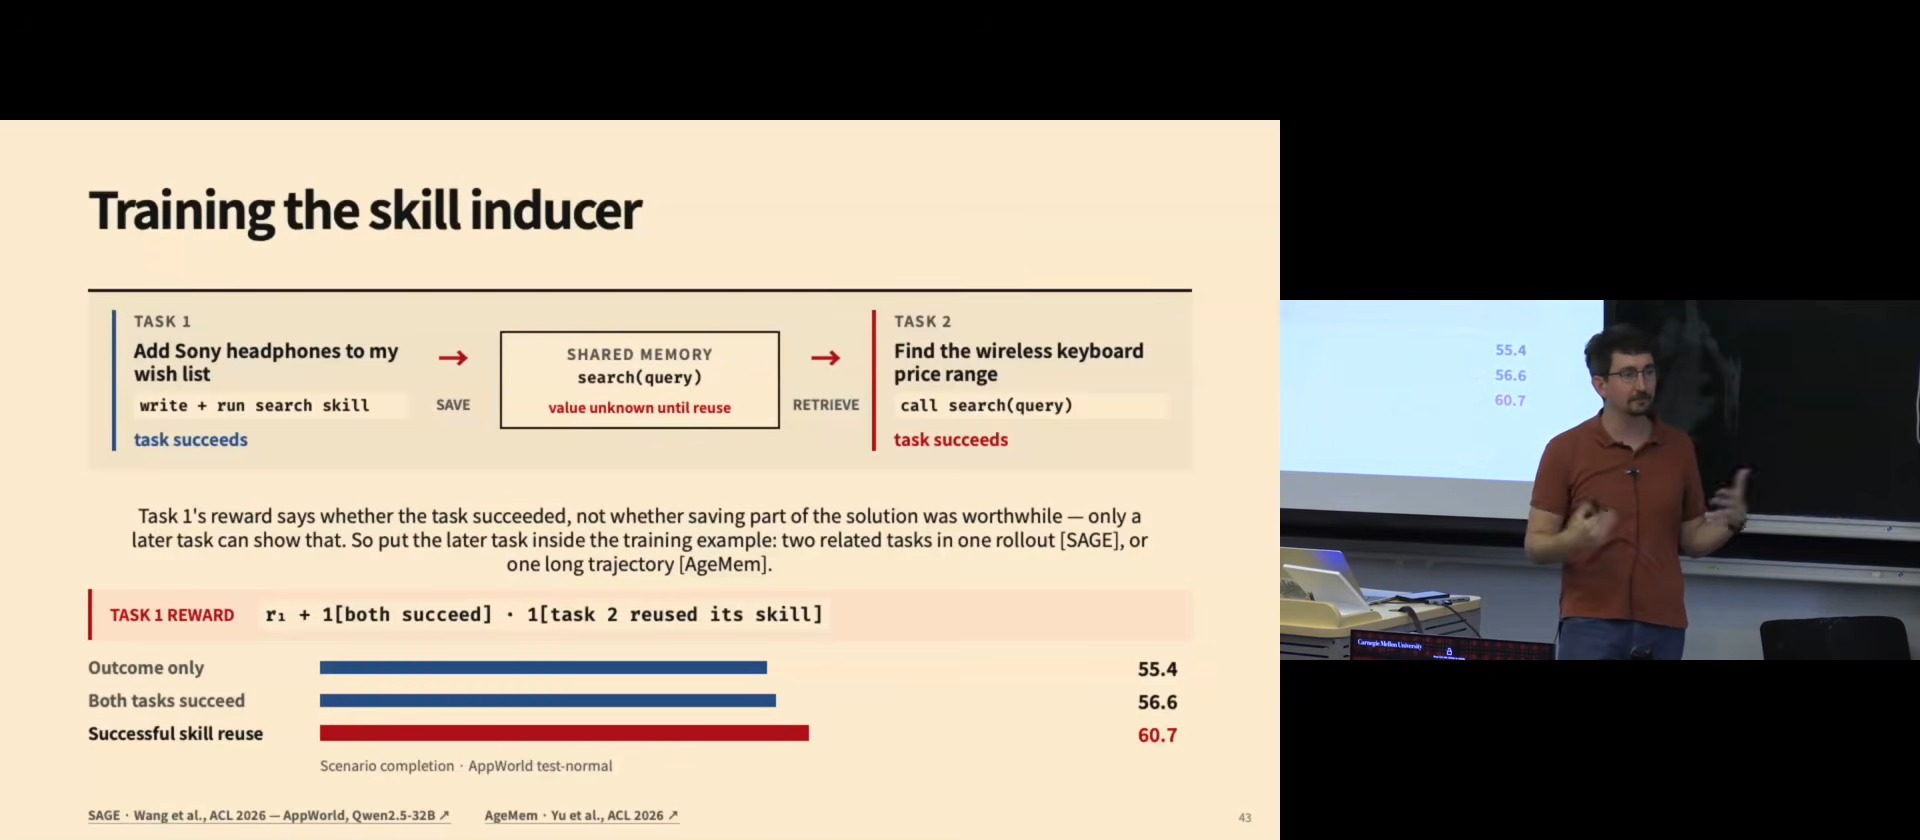
\includegraphics[width=\textwidth]{figures/fig_36_training_skill_inducer.jpg}
\caption{训练技能归纳器：把共享记忆放进强化学习回路，奖励包含“后续任务是否复用技能”，场景完成率随奖励设计从 55.4 提升到 56.6 再到 60.7\vtag}

\end{figure}
\srcnote{01:14:45--01:15:00}

第一个任务的成功本身并不能说明“保存这段技能”是否值得，只有后续任务才能证明它的价值。因此这些工作把后续任务放进同一次 rollout：要么在一次训练样本里放两个相关任务，要么放一条横跨多任务的长轨迹。奖励也随之改进，除了任务是否成功，还额外奖励技能是否被复用：

\[
r_1 = \mathbf{1}[\text{两个任务都成功}] + \mathbf{1}[\text{第二个任务复用了归纳出的技能}].
\]

\begin{itemize}
\item $r_1$：第一个任务的训练奖励；
\item $\mathbf{1}[\text{两个任务都成功}]$：两个任务都完成时取 1，衡量技能是否真的有用；
\item $\mathbf{1}[\text{第二个任务复用了归纳出的技能}]$：技能被实际复用时取 1，鼓励系统产出可复用的产物而非一次性方案。
\end{itemize}

视频给出了三种奖励设定的对照：只看结果时场景完成率为 55.4，加入“两个任务都成功”后为 56.6，再要求“技能被成功复用”后达到 60.7。视频还提到，可以进一步加入惩罚技能库规模的奖励项，以避免技能库过度膨胀。

\begin{knowledgebox}{强化学习为什么能用在这样的流程上}
共享记忆的写入、检索和使用是分不开的整体，中间还夹着文本检索这样的非可微步骤，看起来不适合端到端训练。视频的解释是：强化学习不需要过程可微，只需要能对最终结果打分。于是“把后续任务写进同一次 rollout、用任务成败与技能复用作为奖励”就足以定义训练信号。
\end{knowledgebox}

\subsection{本章小结}

记忆的质量取决于两件事：写进去的内容是否经过正确判定，以及检索出来的内容是否真的相关。失败案例只在被抽象成策略时才有帮助，裁判的不完美会平滑地降低性能，过度检索会主动伤害表现。把归纳器放进强化学习回路，则让系统有机会学会“什么值得保存”。

\section{总结与延伸}

本讲回答了一个问题：智能体如何在上下文窗口之外积累经验，并把它变成可复用的技能。核心结论可以压缩成四点。

第一，可积累的经验有三类：完整轨迹、事实与技能。轨迹保真但昂贵且难以迁移；事实适合稳定、会反复用到的信息；技能是“如何做”的抽象，只在同一子过程重复出现时才有价值。三者不是互相替代的关系，而是服务于不同的复用距离。

第二，外部工件相对上下文窗口和模型权重有一个不可替代的优势：可检查、可编辑、可移植。代价是它必须被主动归纳、筛选和维护。MemGPT 的分层存储与工具驱动读写给出了骨架，冲突更新机制补上了一致性，避免过期事实与最新事实同时被检索。

第三，技能的表示法决定它的强项与边界。文本技能灵活，不提升效率；代码技能可执行、可组合、高效，但容易在环境变化时失效。把两者放进同一个技能包，是目前标准允许的做法，而如何组合仍然是一个开放问题。评测给出了一个不依赖于个例的基线：人工技能把平均通过率从 33.9 提升到 50.5，但增益集中在所需技能较少、SKILL.md 较短的任务上，并且技能在 87 个任务中的 13 个上仍然有害。

第四，记忆的收益不是单调的。过度检索会让成功率下降，失败案例只有在被抽象成文本策略时才有帮助，整理记忆反而能同时改善效率与性能。这些现象共同说明，记忆系统的设计目标不是记住一切，而是让正确的经验在正确的时刻以正确的形态出现。

视频最后把三个问题交还给听众：什么经验应当被存成轨迹、事实、策略、文本技能还是代码；智能体应当在什么时候删除或修订一个技能；在技能的创建与使用上，人与智能体应当如何分工。用本讲的证据回答，可以给出三条可操作的判据。其一，如果同一子过程会反复出现且规格稳定，就把它固化成技能，优先考虑代码表示并在环境多变时保留文本表示。其二，收录前必须有判定闸门，运行后必须有维护入口，因为错误的正例和过期的技能都会被反复复用。其三，检索预算要保守，只取确实相关的条目，因为多召回一条不相关经验带来的干扰，往往大于它可能提供的信息。

从课程的推进看，本讲把“记忆”放在了上下文管理与模型微调之间：它比上下文窗口持久，比微调灵活，代价是引入了检索质量与判定质量这两个新的不确定性来源。接下来自然会追问：当记忆中的技能积累到成百上千条时，如何让检索本身变得可靠，以及如何把归纳、检索与使用放进一个统一的训练目标里。

\end{document}
